\documentclass[prodmode,acmcsur]{acmsmall} 
\usepackage{microtype}
\usepackage{paralist}
\usepackage{tikz}
\usepackage{amsfonts}
\usetikzlibrary{backgrounds}
\usetikzlibrary{snakes}
\usepackage{appendix}
\usepackage{tabularx}
\usepackage{multirow}
\usepackage{amsmath}
\usepackage{tikz}
\usepackage{float}
\usepackage{tabularx}
\usepackage{graphicx}
\usepackage{epstopdf}
\usepackage[scriptsize]{subfigure}
\usepackage{booktabs}
\usepackage{rotating}
\usepackage{listings}
\usepackage{rotating}
\usepackage{paralist}
\usepackage{setspace}
\usepackage{booktabs}
\usepackage{arydshln}
\usepackage{breqn}
\usepackage{mathtools}
\usetikzlibrary{trees,matrix,fit,shapes,calc}
\usepackage{array,multirow}
\usepackage{tikz-qtree}
\usepackage{epstopdf}
\usepackage{xspace}
\usepackage[colorinlistoftodos,prependcaption,textsize=tiny]{todonotes}

\newenvironment{notproof}[1][\proofname]{\proof[#1]\mbox{}\\*}{\endproof}


\newcommand{\tuple}[1]{\ensuremath{\left \langle #1 \right \rangle }}
\newcommand{\la}{\ensuremath{ \mathcal{L}}}
\newcommand\clearemptydoublepage{{\pagestyle{empty}\cleardoublepage}}
%\newcommand\todo[1]{{\color{red}TODO: #1}}
\newcommand\tocheck[1]{{\color{blue}#1}}
\newcommand\m[1]{\mathcal{#1}}
\newcommand{\fl}[1]{\lfloor #1 \rfloor}
\newcommand{\ce}[1]{\lceil #1 \rceil}
\newtheorem{property}[theorem]{Property}
\newcommand{\ngr}[1]{{\color{red}#1}}
\newcommand{\ceil}[1]{\ensuremath{\left\lceil{#1}\right\rceil}}
\newcommand{\floor}[1]{\ensuremath{\left\lfloor{#1}\right\rfloor}}
\newcommand{\LD}{\ensuremath{ \mathcal{LD}}}
\newcommand{\cs}{\ensuremath{ \mathcal{CS}}}
\newcommand{\nat}{\ensuremath{ \mathbb{N}}}
\newcommand{\MC}{\ensuremath{ \mathcal{MC}}}
\newcommand{\BC}{\ensuremath{ \mathcal{BC}}}
\newcommand{\LS}{\ensuremath{ \mathcal{LS}}}
\newcommand{\pre}{\operatorname{pre}}
\newcommand{\dfs}{\operatorname{dfs}}
\newcommand{\dfsi}{\operatorname{dfs_i}}
\newcommand{\dfsd}{\operatorname{dfs_d}}
\newcommand{\bin}{\operatorname{bin}}
\newcommand{\emptystring}{\varepsilon}



\newcommand{\lex}{<_{\text{lex}}}
\newcommand{\s}[1]{\ensuremath{\mathtt{#1}}}
\newcommand{\zero}{\s{0}}
\newcommand{\one}{\s{1}}

%functions
\newcommand{\adjacency}{\emph{Adjacency}\xspace}
\newcommand{\nonadjacency}{\emph{Non-Adjacency}\xspace}
\newcommand{\siblings}{\emph{Siblings}\xspace}
\newcommand{\ancestry}{\emph{Ancestry}\xspace}
\newcommand{\nonancestry}{\emph{Non-Ancestry}\xspace}
\newcommand{\NCAf}{\emph{Id-NCA}\xspace}
\newcommand{\NCAl}{\emph{Label-NCA}\xspace}
\newcommand{\NCA}{\emph{NCA}\xspace}
\newcommand{\flow}{\emph{MaxFlow}\xspace}
\newcommand{\centerf}{\emph{Center}\xspace}
\newcommand{\routing}{\emph{Routing}\xspace}
\newcommand{\distance}{\emph{Distance}\xspace}
\newcommand{\seplevel}{\emph{SepLevel}\xspace}
\newcommand{\connectivity}{\emph{Connectivity}\xspace}
\newcommand{\smalldistance}{\emph{Small-Distance}\xspace}


\newcommand{\ldepth}{\operatorname{ldepth}}
\newcommand{\lpath}{\operatorname{lpath}}
\newcommand{\parent}{\operatorname{parent}}
\newcommand{\siblingsop}{\operatorname{siblings}}
\newcommand{\children}{\operatorname{children}}
\newcommand{\ancestors}{\operatorname{ancestors}}
\newcommand{\descendants}{\operatorname{descendants}}
\newcommand{\depth}{\operatorname{depth}}
\newcommand{\rpath}{\operatorname{rpath}}
\newcommand{\apex}{\operatorname{apex}}
\newcommand{\llabel}{\operatorname{llabel}}
\newcommand{\hlabel}{\operatorname{hlabel}}
\newcommand{\flabel}{\operatorname{label}}
\newcommand{\hpath}{\operatorname{hpath}}
\newcommand{\hchild}{\operatorname{hchild}}
\newcommand{\lchildren}{\operatorname{lchildren}}
\newcommand{\lsiblings}{\operatorname{lsiblings}}
\newcommand{\lsize}{\operatorname{lsize}}
\newcommand{\size}{\operatorname{size}}
\newcommand{\Id}{\operatorname{Id}}
\newcommand{\Ap}{\operatorname{Ap}}
\newcommand{\Range}{\operatorname{Range}}
\newcommand{\app}{\operatorname{Approx}}
\newcommand{\NCAfixed}{\operatorname{NCA-fixed}}

\usepackage[noend]{algpseudocode}

\begin{document}
\title{A Survey on Labeling Schemes for Trees}
\author{Stephen Alstrup, Esben Bistrup Halvorsen and Noy Rotbart}

\begin{abstract}
A labeling scheme is a method of labeling the nodes of a graph so that queries concerning nodes can be answered efficiently directly from their labels. 
For the last 25 years, labeling schemes have been investigated, and they play an important role in the theory of distributed data structures.
The two main characteristics of a labeling scheme are: the type of queries that can be answered from the labels; and the family of graphs which the labeling scheme can accept as input. 
The primary indicator of quality of a labeling scheme is the size of the labels  it produces.
We survey the literature on   lower and upper bounds for the worst-case sizes of labels produced by labeling schemes for trees.
In addition, we present selected  techniques and results that achieve the best known lower and upper bounds as well as selected variants thereof.
The survey presents the results systematically on a standard selection of families of trees. 
\end{abstract}

\keywords{Labeling schemes, Induced universal graphs}


\begin{bottomstuff}
\end{bottomstuff}

\maketitle

\section{Introduction}
% !TEX root = ../Survey.tex
The Internet is a  large, geographically dispersed network, and information about its structure is needed by all its participants.
Decentralizing the structural information is a key part in its scalability and performance.

Labeling schemes allow the structure of a  graph to be distributed among its nodes  such that certain queries can be answered in a short time.
Moreover, the information needed to answer the queries should be contained in the labels of the questioned nodes themselves.
On the one hand, storing the entire data structure at each node would result in short answer time for each query.
On the other hand, such replications would defy the aim of distributing information.
Therefore, the primary indicator of the quality of a labeling scheme is the size of the labels it produces in the worst-case scenario.

 The papers surveyed are built for specific types of queries. \adjacency \todo{I don't think ``adjacency'' should be written like this all over the place (but it's fine to have it slanted here).} labeling schemes were the first to be investigated in the literature. The nodes in a graph  are labeled in such a way that the \adjacency between two nodes can be determined directly from their labels. A restricted form of \adjacency labeling schemes for graphs was studied almost 50 years ago by \citeN{Breuer67}. The more general concept  was defined 25 years later by Kannan, Naor and Rudich~\shortcite{Kannan92} as well as by \citeN{Muller1988}. Following that, the idea laid dormant for over a decade until it was noticed that labeling schemes could also be defined for many other types of queries other than \adjacency. This observation revived interest in labeling schemes and triggered an abundance of subsequent publications, including many variants of the concept. Further detail on the historical development of labeling schemes can be found in~\cite{Peleg03}.

This survey considers labeling schemes for the family of trees with at most $n$ nodes. We focus on this particular family for the following reasons: 
When graphs are considered, labeling schemes for all of  the  functions we are surveying require a  label size that is in the  order of the size of the graph itself. Even for the most basic query, \adjacency, labeling schemes require at least $n/2$ bits to support the family of  graphs~\cite{rado1964universal}.
It is thus not surprising that the focus of the body of work surveyed, and  the early definitions of labeling schemes,  require labels of a size that is poly-logarithmic in the size of the graph. 
On the other hand, techniques introduced in  the papers surveyed  contributed directly to  labeling schemes for several families of  graphs.
Among others, bounded tree-width~\cite{gavoille2007shorter}, bounded degree~\cite{adjiashvili2014labeling}, bounded arboricity~\cite{Alstrup02}, and planar graphs~\cite{Thorup01} labeling schemes  for various functions are obtained directly from their corresponding labeling schemes for trees. 

\subsection{An example} \label{sec:example}
Before diving into practical applications and details of the precise definition of labeling schemes, it is instructive to warm up with a small example accompanied by some general remarks. 
This section therefore presents a simple \emph{\adjacency labeling scheme for trees}: What this means will be made precise later, but the general idea is to construct an algorithm that associates with every node a \emph{label}, which is just some data, such that, given the labels of two nodes, one can determine if the nodes are adjacent or not.

Consider an arbitrary rooted tree with $n$ nodes. Enumerate the nodes in the tree with the numbers $0$ through $n-1$ as binary strings, and let, for each node $v$, $\Id(v)$ be the number associated with $v$ and, when $v$ is not the root, $p(v)$ be the parent of $v$ in $T$.
Consider the labeling $\la(v)= (\Id(v),\Id(p(v))$ of all non-root nodes $v$ and $\la(\Id(r),\Id(r))$ for the root node $r$.
The encoding of the labels is demonstrated in Figure~\ref{fig:simple}.
Note that two nodes $u$ and $v$ are adjacent if and only if either $\Id(p(v))=\Id(u)$ or $\Id(p(u))=\Id(v)$ but not both. Thus it is possible to determine adjacency of $u$ and $ v$ directly from their labels $\la(u)$ and $\la(v)$.

\begin{figure}[!ht]
\centering
\begin{tikzpicture}[scale = 0.7,inner sep=0pt, minimum size=5ex, sibling distance=0.4em]
\tikzstyle{every node}=[draw,circle]
\Tree  [ 
.{1,1} 
	\edge; [.{2,1} [.{3,2} \edge[]; [.{5,3} \node{6,5}; ]
							       [.\node{7,3}; \node{8,7}; \edge; {9,7} ]
                       					       \edge; [.{10,3} \node{11,10}; ]
					    ] 
					    \edge; {4,2} ]
	\edge;  [.{12,1} \node{13,12}; ]
	[.\node{14,1}; \edge; {15,14}
			[.\node{16,14}; \edge; {17,16}
					[.\node{18,16}; \edge; {19,18}
							\node{20,18};
							\edge; {21,18} ]
					\edge; {22,16} ]
			\edge; {23,14} ]
	]
\end{tikzpicture}
\caption{
A tree with $n=23$ nodes. Each node is assigned a label of size $2 \log n$ supporting \adjacency queries. A node $v$ with parent $u$ is labeled $(\Id(v),\Id(u))$ and the root $r$ is labeled $(\Id(r),\Id(r))$.} \label{fig:simple}
\end{figure}

This is a labeling scheme. It consists of an \emph{encoder} algorithm that labels the nodes of a tree and a \emph{decoder} algorithm that can answer \adjacency queries using only labels as input. Note that the encoding algorithm relies on knowing the entire tree, whereas the decoding algorithm only knows the labels it receives as input and nothing else. 

Recall that the quality of a labeling scheme is measured by the size of the label it produces in the worst case.
In the above example, the pair $(\Id(u),\Id(v))$ can be represented as a binary string of length $2\ceil{\log n}$.\footnote{From hereon, unless stated otherwise,  $\log n$ stands for $ \log_{2} n$}% and $n$ is assumed to be a power of $2$.}
%\todo{Do we really want to assume that $n$ is a power of 2? In principle, you cannot know that such an algorithm works for non-powers of 2 (although it most often will).}
The  goal is to find an \emph{optimal} labeling scheme: that is, one where the worst-case label size is as small as theoretically possible.

There are two main characteristics of a labeling scheme. First, there is the type of query for which the labeling scheme has been constructed. In our example, the type of query is ``\adjacency'', but it could also have been something else, for example ``\ancestry'' (is one node an ancestor of the other?) or ``\distance'' (what is the distance between  two nodes?). Second, there is the family of graphs under consideration. In our example, the labeling scheme is for the family of all trees, but both smaller and larger families would have been possible. A different choice of query or a different choice of graph family may lead to an entirely different labeling scheme with different properties and a different optimal worst-case label size. 

\subsection{Outline}
This survey provides an overview of labeling schemes where the maximum (worst-case) label size is as small as possible.
The problem of finding such labeling schemes for a graph family $\mathcal{G}$  for a given function $f$ is known as the \emph{$f$-labeling problem for $\mathcal{G}$}.
We mainly survey results on  the graph family of trees with at most $n$ nodes due to great interest in the literature, with occasional emphasis on several bounded cases (i.e bounded degree, bounded depth, caterpillars and binary trees).
Tables~\ref{table:main} and~\ref{table:bounded} \todo{Why are tables numerated with Roman numerals? It seems a bit inconsistent.} provide a concise description of the results.
An overview of applications for labeling scheme is provided in Section~\ref{section:applications}, and formal definitions are given in Section~\ref{section:preliminaries}.

Let $k \in \mathbb{N}$, and let $T=(V,E)  \in Trees(n)$ \todo{The ``Trees'' should be a LaTeX command - all over the document...} be a tree rooted at the node $r$.
We survey labeling  schemes supporting  the following functions for any  $u,v,w \in V$:
	\begin{enumerate}
	  \setlength{\itemsep}{2pt}
	\item $\adjacency:(V \times V) \rightarrow \{\false,\true\}$ (Section~\ref{section:Adj})  			 \\ $\adjacency_T(u,v) = \true$ if and only if $u$ and $v$ are adjacent in $T$. \todo{It's totally ugly, in my opinion, that all these functions are slanted. Use $\backslash$operatorname or something.}
	\item $\ancestry: (V \times V) \rightarrow \{\false,\true\}$    (Section~\ref{section:Anc})  		  \\ $\ancestry_T(u,v) = \true$ if and only if $u$ is an ancestor of $v$ in $T$.
	\item $\NCA: (V \times V) \rightarrow \{ 0,1 \}^+$       (Section~\ref{section:NCA})  			\\  $\NCA_T(u,v)$ returns the label of the first node in common for the paths  $v \leadsto r $ and $u \leadsto r$ in $T$.  \todo{Do we need to define and point out the uniquess of ``$\leadsto$''?}
	\item $\routing: (V \times V) \rightarrow \nat $        (Section~\ref{section:Routing})  					\\  $\routing_T(u,v)$ returns the port number (Definition~\ref{dfn:port}) leading to the next node on the  path  $u \leadsto v$ in $T$.
	\end{enumerate}
We also discuss the functions \nonadjacency and \nonancestry which are the negated functions of \adjacency and \ancestry. Each section contains a detailed literature overview,  as well as a report on one or more central results presented in some detail. Common for the algorithms presented is that, in most cases, they are  the best known results.

	Labeling schemes for the following  functions are also reported in Table~\ref{table:main} \todo{I think this table should be properly introduced. Otherwise it's a bit weird to write ``also''.} and occasionally mentioned.
	Some of these functions are also defined for the family of edge weighted $n$ node trees, i.e. trees where each edge is assigned an integer at most $2^M$ for some integer $M$.  We denote this family as $WeightedTrees(n,2^M)$. \todo{``WeightedTrees'' should be a LaTeX command}
	\begin{enumerate}	
	\item $\centerf: (V \times V \times V) \rightarrow \{ 0,1 \}^+$      %(Section~\ref{Section:NCA-lowerbound})
	   \\ $\centerf_T(u,v,w)$  returns the unique node $z$ such that the three paths  $z \leadsto u$, $z \leadsto v$, and  $z \leadsto w$  in $T$ are edge-disjoint.
	\item $\distance: (V \times V) \rightarrow \nat$         %(Section~\ref{section:distance})
	  \\ $\distance_T(u,v)$ returns the length of the path  $u \leadsto v $ in $T$, which is  equal to the number of edges in $u \leadsto v$ if $T$ is unweighted. \todo{Do we need to define ``length of the path'' in the weighted case?}
	\item $\flow: (V \times V) \rightarrow \nat$         %(Section~\ref{section:distance})   	
	\\ $\flow_T(u,v) $ returns the smallest edge weight on $ u \leadsto v$  in $T$.
	\item $\siblings: (V \times V) \rightarrow \{false,true\}$       % (Section~\ref{section:Sib}) 
	 \\ $\siblings_T(u,v) = true$ if and only if  the parent of $u$ is the parent of $v$ in $T$ for $u \neq r$ and $v \neq r$. A node is its own sibling. \todo{I'm not sure that is the standard definition. The labeling problem is different in the two cases---uniqueness is not required!}
	\item $\seplevel: (V \times V) \rightarrow  \{ 0,1 \}^+$        (Section~\ref{sec-NCA-FIXED}) 			  \\ $\seplevel_T(u,v)$ returns the length of the path  $r \leadsto w $ in $T$ where $r$ is the root and $w$ is $NCA_T(u,v)$.
	\item $\smalldistance: (V \times V \times \nat) \rightarrow \nat$    
	\\ $\smalldistance_T(u,v,k)= true$  if and only if $\distance_T (u, v) \leq k$ in $T$, otherwise, it returns $\infty$.
	\end{enumerate}
	
See Figure~\ref{fig:complexityruler} for an illustration of the number of bits required for labeling schemes for each of these functions.
In the course of the survey, we provide missing details and correct minor mistakes found in the literature surveyed.
We also present an improved labeling scheme for the function \ancestry in Section~\ref{subsetion:mat-optimal}.

\begin{table}
\tbl{Known upper and lower bounds for efficient  labeling schemes on trees. Labeling schemes that do not necessarily provide unique labels  are marked with *.The families  $Trees(n), Forests(n), BinaryTrees(n),Trees(n, \delta)$ and $Trees(n, \Delta)$ are formally defined in Section~\ref{section:preliminaries}. Results implied, but not specified in the literature are marked with $^{\dagger}$.}{
\begin{tabular}{cccccc}
    Reference &Variant  & Upper bound	&Lower bound	  & Encoder & Decoder    \\ \hline\hline
&&\underline{\adjacency} \\ \\
\cite{alstrup2015optimal}		&$Trees(n)$  &$\log n+O(1)$ 		&$\log n+ 1$ 			 &$O(n)$ 			& $O(1)$\\ 
\cite{Gavoille06} &$BinaryTrees(n)$    &$\log n+O(1)$  		 &$\log n+ 1$		 	& $O(n)$	            	&$O(1)$ \\ 
\cite{Fraigniaud10}	&$Trees(n, \delta)$ 		  &$\log n+3 \log \delta+O(1)$   &$\log n+ 1$	& $O(n)$	            	&$O(1)$  \\ 	
\cite{adjiashvili2014labeling}	&$Trees(n, \Delta)$ 	   &$\log n+O(\log \Delta)$  &$\log n+ 1$	& $O(n \log n)$	            	&$O(\log\log n)$\\ 						
			
%			 &One sided error*			& $2(k+1) $ with	 	  					& $\log n + \log p - O(1)$	 & $O(n)$ 		        & $O(1)$ 			&\cite{fraigniaud2009} \\ 
%			&   						&$p= 1-\frac{1}{2^k}$						&		\\ 
&&\underline{\nonadjacency} \\ \\
\cite{fraigniaud2009} &One sided error* & $2k+1$ with 	&$---$	 & $O(n)$ 		        & $O(1)$ \\ 
&&$p= 1-\frac{1}{2^k}$\\ 	\hline
&&\underline{\ancestry} \\ \\
\cite{dahlgaard2014improved}&$Trees(n)$	 &$\log n +2 \log \log n+3$	 	  		&$\log n+ \log \log n$& $O(n)$ 		        & $O(1)$ \\ 
\cite{Fraigniaud10} &$Trees(n,\delta)$	&$\log n +2 \log \delta+ O(1) $	&   & $O(n)$ 		        & $O(1)$ \\ 
\cite{fraigniaud2009}	&One sided error*   			& $\log n - \frac{k}{2}+ O(\log \log n)$& $\log n + \log p -$	& $O(n)$ 	& $O(1)$ \\ 
&& with $p=\frac{1}{2^k}$	&$O(1)$\\ 				
&&\underline{\nonancestry}\\ \\
\cite{fraigniaud2009}&One sided error*  & $\lceil \log n \rceil $ with 	& $\log n + \log p -$	 & $O(n)$ 		        & $O(1)$ \\ 
&&  $p=\frac{1}{2}$	&$O(1)$\\ \hline			
&&\underline{\centerf} \\ \\
\cite{Peleg05} &$Trees(n)$, fixed model &$\Theta(\log^2 n)$ 	&$ \Theta(\log^2 n)$		 & $O(n \log n )$	  		&$O(1)^{\dagger}$ \\ \hline
&&\underline{\connectivity}\\ \\ 
 \cite{Alstrup05} &$Forests(n)$		&$\log n+\log\log n  $ & $\log n+\log\log n$ 	 & $O(n)$	  		&$O(1)$ \\ 
 \cite{Alstrup05} &$Forests(n)  $*	&$\log n $		 		& $\log n$ 	 & $O(n)$	  		&$O(1)$ \\ \hline

&&\underline{\distance}\\ \\	
\cite{freedman2016optimal}&$Trees(n)$   &$\frac{1}{4}\log^2 n+o(\log^2 n)$  &$\frac{1}{4}\log^2 n - O(\log n)$  & $O(n \log n)$     & $O(1)^{\dagger}$\\ 
\cite{Gavoille2001}&$WeightedTrees(n,2^M)$  &$\Theta(M \log n + \log^2 n)$	&$\Theta(M \log n + \log^2 n)$	  & $O(n \log n)$    & $O(\log n)$\\  \hline

&& \underline{\distance, approx. $1+1 / n$} \\ \\
\cite{Katz00} &$2^M$ weighted diameter &$\Theta(\log n \cdot \log M)$ 	&$\Theta(\log n \cdot \log M)$ 	 & $O(nm)$ & $O(1)$ \\ 
\cite{Katz00}& $Trees(n)$	&$\Theta(\log n \cdot \log \log n )$&$\Theta(\log n  \log \log n)$  &$O(n \log n)$ &$O(1)$\\ 	\hline
		
&&\underline{\flow} \\\\
\cite{katz2004labeling}&$WeightedTrees(n,2^M)$  &$\Theta(M \log n + \log^2 n)$  &$\Theta(M \log n + \log^2 n)$	& $O(n)$    & $O(1)$ \\ \hline

&&\underline{\NCA} \\ \\
\cite{Green14}&$Trees(n)$, \NCAl	&$ 3 \log n$	&$1.008\log n $	& $O(n)$	     		& $O(1)$ \\ 
\cite{Peleg05}&$Trees(n)$, \NCAf			 &$O(\log^2 n)$	  &$\Omega(\log^2 n)$ 		 & $O(n \log n)$	& $O(1)^{\dagger}$ \\ \hline

&&\underline{\routing} \\ \\
\cite{Thorup01}&$Trees(n)$, designer port  &$(1+o(1))\log n$  & $\log n + \log \log n$ 		& $O(n \log n)$	  		&$O(1)$  \\ 
\cite{Fraigniaud01}&$Trees(n)$, fixed port	  & $\Theta(\log^2 n/\log\log n) $  & $\Theta(\log^2 n/\log\log n)$ 	 & $O(n)$	  &$O(1)$  \\ \hline

&&\underline{\siblings} \\ \\ 
\cite{lewenstein2013succinct}&$Trees(n)$	&$\log n+ \log\log n $	& $\log n+ \log\log n$ 	 & $O(n)$	  		&$O(1)$ \\ 
\cite{Alstrup05}	&$Trees(n)$*	&$\log n $		 & $\log n$ 	 			& $O(n)$	  		&$O(1)$  \\ \hline
						
&&\underline{\smalldistance} \\ \\
\cite{freedman2016optimal} &$Trees(n)$,distance $k$  &$ \min{\log n+O(k \log (\log n/k))} $	&$\log n+\Omega(k \log(\log n/(k \log k)))$	  & $?$    & $O(1)$\\ 
&&	$O(\log n \cdot \log(k/\log n))$	 \\  \\		 
  \end{tabular}} \label{table:main}
\end{table}

				\begin{figure}
				\centering
				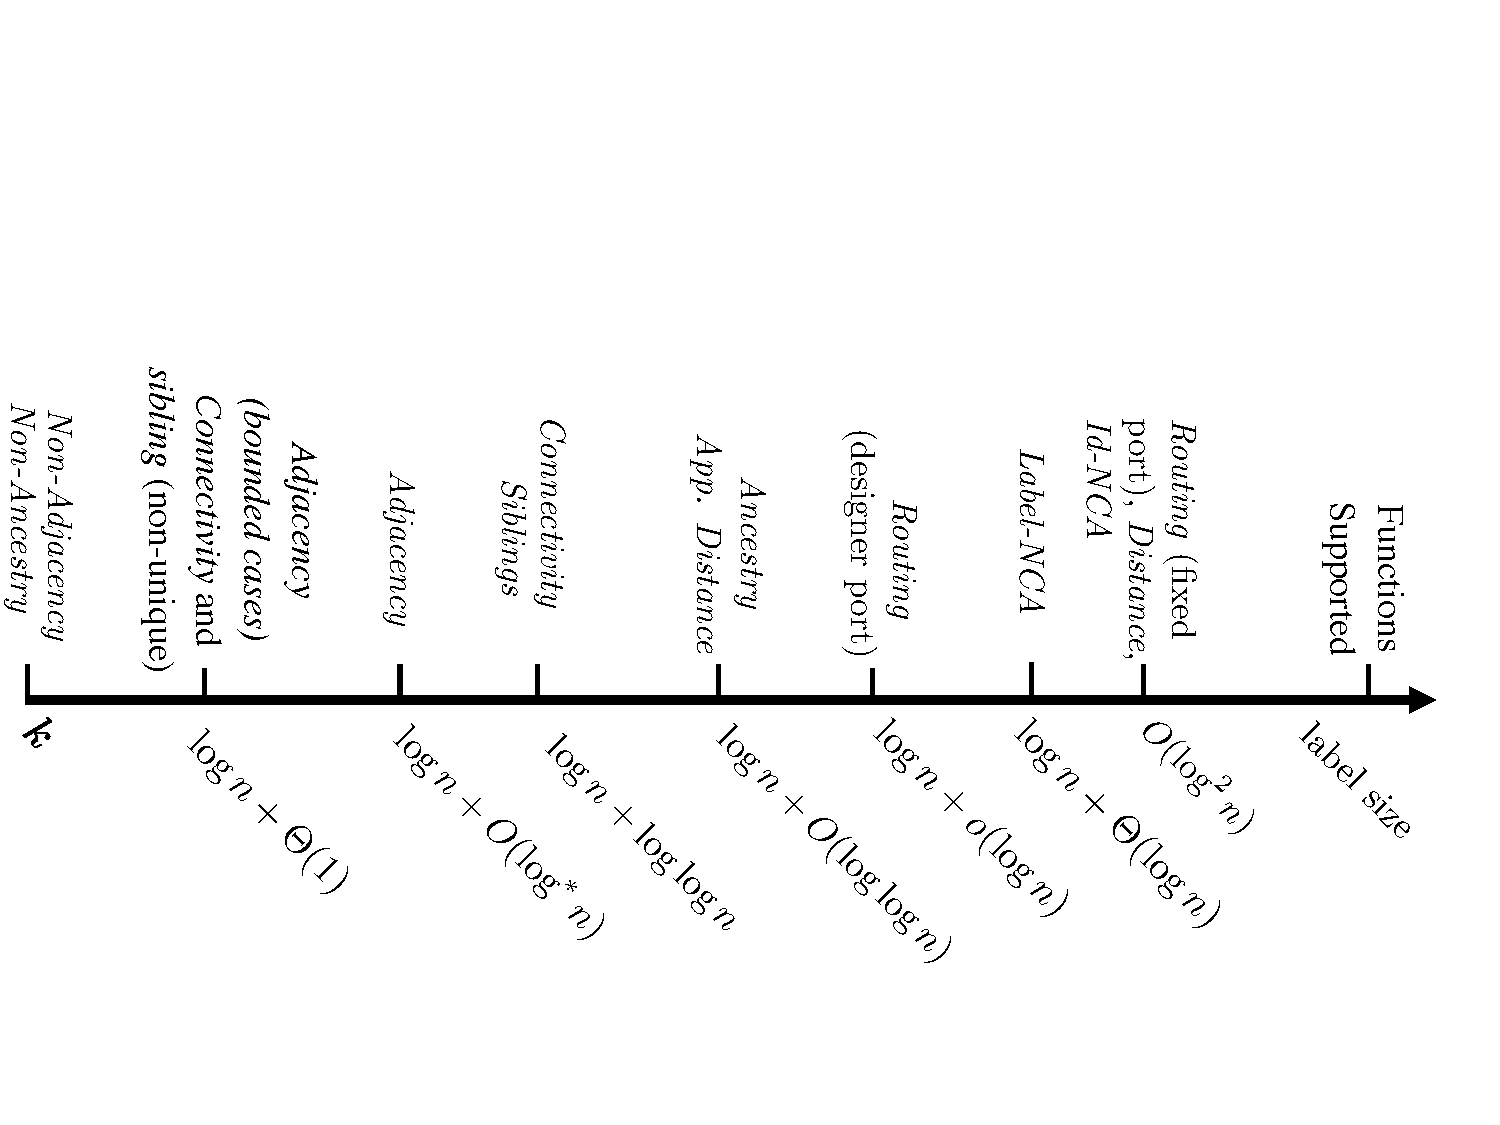
\includegraphics[width=100mm]{./Figures/Hierarchy2.pdf}
				\caption{Given a certain label size, the illustration describes  which operations may be  supported.  }
				\label{fig:complexityruler}
			\end{figure}
			
\todo{Comment to Table I: There is also a less efficient NCA labeling scheme with smaller labels}

\paragraph{Bounded trees}\label{section:Limited}
In Table~\ref{table:bounded}  we complete the description of the following cases: $Caterpillars(n)$, $Trees(n,\delta)$, $Trees(n,\Delta)$, and  $BinaryTrees(n)$, where $\Delta$ refers to maximum degree, $M$  to $2^M$ edge weights, and $\delta$  to  maximum depth.
Note that the table is transposed compared to Table~\ref{table:main}.
We chose to present the results in this fashion  since the  focus is  on the restricted families.
\begin{table}[!ht]
\tbl{Known upper and lower bounds for  labeling schemes on trees with unique encoder.}{
  \begin{tabular}{lcccccc}
    \hline
    &\adjacency 			  & \ancestry		 &\distance			 & \NCA	  		& \siblings   \\ \hline
    \hline
$Caterpillars(n)$: \\
Upper bound	&$\log n +\Theta(1)$  &$\log n +O(1)$  &$2 (\log n + M) $	&$\log n + \log \log \Delta + O(1) $ 	 	&$\log n +O(\log \log n)$\\
& \cite{Gavoille06}	 &  & && \cite{Alstrup05}  \\	\hdashline	

Lower bound	&$\log n + \Theta(1)$ &	$\log n + \Theta(1)$		 &$\log n + \Theta(1)$&	$\log n + \Theta(1)$	& $\log n +\Omega(\log \log n)$	\\ 
&&&&&\\ \hline 

$BinaryTrees(n)$:\\
Upper bound &$\log n +O(1)$ 	 &$\log n +\Theta(\log \log n )$  &$\frac{1}{2}\log^2 n +O(\log n)$&$ O(\log n)$\cite{Alstrup02NCA}&$ \log n +\Theta(1)$  \\ 
&\cite{Gavoille06}	&[Fraigniaud et al. 2010b]&\cite{Gavoille2001}	&\cite{Alstrup02NCA}	&\\ \hdashline   
Lower bound		&$\log n + \Theta(1)$					&$\log n +\Theta(\log \log n)$	  	    &$\frac{1}{8}\log^2 n-O(\log n)$&$\log n + \Theta(1)$	&$\log n + \Theta(1)$	\\ 
&&	&\cite{Gavoille2001}	&		&	\\ \hline 
				
$Trees(n,\Delta)$:\\
Upper bound 	&$\log n +O(1)$ & $\log n +\Theta(\log \log n) $ & $\frac{1}{2}\log^2 n +O(\log n)$ & $O(\log n)$ &$\log n + \Theta(\log \log \Delta)$\\ 
&[Adjiashvili et al. 2014]& [Fraigniaud et al. 2010b] &\cite{Gavoille2001}&\cite{Alstrup02NCA}&\cite{Alstrup05} \\\hdashline

Lower bound &$\log n + \Theta(1)$ &$\log n + \Theta(1)$ &$\frac{1}{8}\log^2 n-O(\log n)$  &$ \Omega(\log n)$	&$\log n$	\\ 
&&&\cite{Gavoille2001}&\cite{Alstrup02NCA} \\
\hline 
			
$Trees(n,\delta)$:\\
Upper bound & $\log n + 3 \log d +O(1)$ &$\log n +2 \log \log d +O(1) $ &$\frac{1}{2}\log^2 n +O(\log n)$ 	&$\log n +O(1)$ 	&$\log n+ \Theta(\log \log n)$\\ 
& [Fraigniaud et al. 2010b] &[Fraigniaud et al. 2010b]	&&& \cite{Alstrup05}\\	\hdashline				

Lower  bound & $\log n + \Theta(1)$	&$\log n + \Theta(1)$  &$\log n + \Theta(1)$  &$\log n + \Theta(1)$  &$\log n + \Theta(\log \log n) $  \\ 
&&&&& \\ \hline						
  \end{tabular}}\label{table:bounded}
\end{table}

\todo{Comment to Table II: It's not the encoder that is ``unique''}	

\todo{Comment to non-existing table: What about all the other variations of labeling schemes, e.g. approximation, probabilistic etc.?}	

						
\subsection{Practical and theoretical applications of labeling schemes}\label{section:applications}
Labeling schemes have  contributed directly to a number of areas, including XML querying, graph theory, shortest paths in road networks and routing schemes.

\paragraph{XML querying}  
 Extensible Markup Language (XML) documents are a popular and ubiquitous standard for exchanging structured data on the Internet~\cite{Kaplan01}. An XML document can be viewed as a rooted tree in which each node corresponds to a semantic element, enclosed by matching beginning and end tags in the form $\verb+<item>+\dots\verb+</item>+$. When searching for information in an XML document, one will typically not only search for pure text but also utilize the semantic structure of the document and specify, for example, certain ancestry relations in the document tree. By using a labeling scheme, queries of this type can be answered directly from labels, which can be stored in a hash table, without having to access the actual document. 
 This can have a significant positive impact on performance, and has been studied extensively~\cite{Cohen02,lu2013xml,harder2007node,Kaplan01,wu2004prime,cohen10journal}.

To achieve a good performance for  queries on  XML documents, it is important  that a large  part of the document's indexed structure can reside in main memory. Since these structures can be extremely large, every single bit counts.
Much of the work in this particular direction focused on seemingly small benefits. For example, both relations used by practitioners, namely, adjacency (illustrated in Figure~\ref{fig:simple}) and ancestry  had strikingly simple  labeling schemes with labels of at most $2 \log n$ bits~\cite{Kannan92}.
In order to identify the XML element uniquely, the label of an element  in an XML file with at most $n$ elements requires at  least  $\log n$ bits. 
The effort to reduce the single additive $\log n$ \todo{You just argued that it cannot be reduced. I guess you mean everything in addition to the $\log n$.} contributed  not only to the performance of XML queries but also to the subject of implicit representation of trees.

\paragraph{Graph theory}
If the query type supported by a labeling scheme allows the entire graph to be reconstructed from the labels, then the collection of labels can be seen as an \emph{implicit representation} of the graph: that is, a representation where the graph is not stored as a single structure but can be determined from a collection of smaller structures.
This is in contrast to any global representation of a graph, for example an adjacency matrix, where the adjacency between two nodes is determined by consulting the relevant entry in a single entity, and where the index of each node contains no relevant information in itself but serves only as a placeholder or a pointer to the entries of the matrix. 
In this sense, a labeling scheme is more efficient since it does not waste space on meaningless placeholders. This, however, does not mean that the collection of labels in total uses less space than a traditional representation: on the contrary, the extra requirement that the data structure must be distributed may lead to one that is  larger in total. 

\citeN{Kannan92} noticed the tight correlation between adjacency labeling schemes and induced-universal graphs. Induced-universal graphs is  a mathematical subfield of implicit graph representations and has been researched extensively since the 1960's~\cite{rado1964universal}. 
For various numbers of families, the goal is to find the smallest number of nodes required for a graph that contains each of the $n$-node graphs of the family  as induced subgraphs. 
 A subsequent connection between universal matrices and \distance labeling schemes was studied by \citeN{Rodeh10} and \citeN{Paul01}.
We defer further discussion on the nature of the connection to Section~\ref{section:Adj}.

\paragraph{Shortest paths in road networks}
Another practical aspect of labeling schemes concerns distributed shortest paths  on road networks. 
\citeN{Gavoille2001} first investigated \distance labeling schemes. 
Abraham, Deiling, Goldberg and Werneck \shortcite{abraham2010hub,abraham2012hierarchical} modified the labeling schemes to achieve a distributed system to answer reachability and shortest path queries on road networks.

\paragraph{Routing schemes}
Perhaps the most  practical application of labeling schemes arises from  routing schemes.
In a large network, information sent from one participant  to another must visit   other participants in the network according to the network topology. 
A routing scheme is a description of a  system designed to support the operation of transferring packets through the network.
According to \citeN{Peleg05}, labeling schemes  assist in the design of ``memory-free'' routing schemes, which support fast and simple switch architectures by  storing  little data locally.
 A significant effort by the community yielded numerous  papers dealing with labeling schemes for routing \cite{Peleg03,Thorup01,Fraigniaud01,gavoille96,Dom07,Korman07K,krioukov2004compact,abraham2006routing,abraham2005name}.





\subsection{Preliminaries}\label{section:preliminaries}
In the remainder of the paper we use the following terms:
			$k$ is a positive integer.
			A binary string is a member of the set $\{ 0,1 \}^*$.
			We define $\ceil { \log_2{n}}$ as $\log{n}$.   %\todo{Really? Maybe you mean that we \emph{define} $\log n$ to mean $\ceil{\log_2 n}$?}
			We denote by $\mathbb{N} = \{1,2 \dots \} $ the set of natural numbers and by $\mathbb{N}_0 = \{0,1,2 \dots \} $ the extended set that includes $0$.
			For $x \in \mathbb{N}$ we denote by $\bin(x)$ its standard binary representation, and $\vert x \vert$ as the number of bits in $\bin(x)$. \todo{The latter seems like a really dangerous and weird definition. Then we have e.g. $\vert 4\vert=3$.}
			The concatenation of two bit strings $a$ and $b$ is denoted $a \circ b$.
			\subsubsection{Graph families related definitions} 
			For a graph $G$ we denote the set of nodes and edges by $V(G)$ and $E(G)$, respectively.
			For any graph family $\mathcal{F}$, let $\mathcal{F}(n) \subseteq \mathcal{F}$ denote the subfamily containing the graphs of at most $n$ nodes.
			Unless stated otherwise, the number of nodes in a graph $n$ is assumed to be a power of $2$. \todo{Again, I think this is somewhat restrictive}
			The family of all graphs is denoted $\mathcal{G}$.
			 The collection of unweighted forests in $\mathcal{G}$ respectively~$\mathcal{G}(n)$  is  denoted $Forests$ respectively~$Forests(n)$. \todo{Make a LaTeX command for ``Forests''}
			The collection of unweighted trees in $Forests$ respectively~$Forests(n)$  is  denoted $Trees$ respectively~$Trees(n)$.
			Similarly,  the  collection of edge weighted trees, with weights in $\{1 \dots 2^M \}$  in $\mathcal{G}$ respectively~$\mathcal{G}(n)$ is denoted $WeightedTrees(2^M)$ respectively~$WeightedTrees(n,2^M)$.
			A \emph{caterpillar} is a tree in which all non-leaf nodes lie on a single path, denoted the \emph{main path}. The collection of unweighted caterpillars in $Trees$ respectively~$Trees(n)$  is denoted $Caterpillars$ and $Caterpillars(n)$.
			The collection of trees with bounded depth $\delta$ in $Trees$ respectively~$Trees(n)$  is  denoted $Trees(\delta)$ respectively~$Trees(n,\delta)$.
			Trees of  Bounded degree $\Delta$  are marked similarly $Trees(\Delta)$  and $Trees(n,\Delta)$.
			As a shorthand, trees of bounded degree $3$ are marked $BinaryTrees$ and $BinaryTrees(n)$. \todo{If trees are rooted, this may not be the correct definition}
			For each of the (unbounded) families described the bounded degree and depth variants are denoted in according.
			From hereon, unless stated otherwise, we assume trees to be rooted. 

	\subsubsection{Basic tree related definitions} \label{definitions-of-trees}
	Let $T=(V,E) \in Trees(n)$ be a tree rooted in $r$. The number of edges in a tree is always $|E|=|V|-1$. The nodes of degree $1$ other than the root are called \emph{leaves}, and all other nodes are called \emph{internal} nodes.
	
	Let $u$ and $v$ be nodes in  tree $T$. 
	If $(v,u) \in E$ \todo{Since edges have no direction, I think the correct definition would be $\{v,u\}$} we say that $v$ and $u$ are  \emph{neighbours}. We denote  the set of all neighbours of $v$ as $N(v)$, and the degree $\vert N(v) \vert$ of $v$ as $\deg(v)$.  A non-root node with degree at most $1$ is called a  \emph{leaf}, and an \emph{inner node} is a non-leaf node. The parent of $v$, if $v$ is not the root, is denoted $p(v)$, and $v$ is the \emph{child} of $p(v)$.  A \emph{sibling} $v \neq u$ of $u$  is a child of $p(u)$.
	We denote by $v \leadsto u$ the  sequence  \tuple{v_0,v_1 \dots v_k} of vertices such that $v = v_0$, $u = v_k$, and $(v_{i-1},v_{i})\in E$ for $ i= 1,2 \dots k$ between $v$ and $u$ in $T$. \todo{Can there be duplicates? If yes, then paths are not unique.}
	This sequence is typically called the \emph{path} between $v$ and $u$, and $k$ is called the \emph{length} of the path $v \leadsto u$. Note that   every two nodes in a tree are connected by a unique path.
The distance between $u$ and $v$ in $T$, denoted $\distance(u, v)$, is the number of edges on the path  $u \leadsto v $. The distance from  $v$ to the root is called the \emph{depth} of $v$, denoted $\depth(v)$, and the depth of the tree, $\depth(T)$, is the maximum depth among its nodes.
	If $u$ is a node on the path from the root of a rooted tree to a node $v$, then $u$ is an \emph{ancestor} of $v$, and $v$ is a \emph{descendant} of $u$. Note, in particular, that a node is its own ancestor, descendant and sibling, but not its own child or parent. A \emph{common ancestor} of two nodes is a node that is an ancestor of both nodes, and their \emph{nearest common ancestor} (NCA) is the unique common ancestor with maximum depth. Given a node $v$, the descendants of $v$ form an induced subtree $T_v$ with $v$ as root.  Finally, the \emph{size} of $v$, denoted $\size(v)$, is the number of nodes in $T_v$.
	
	Additional standard definitions are provided in Appendix~\ref{AppendixA}.
\subsubsection{Labeling schemes and variations} 
We present definitions of labeling schemes, approximation labeling schemes and one-sided error labeling schemes.			
\begin{definition}\label{dfn:labeling_schemes}
Let $f : V(G)^k  \rightarrow S$ be a k-ary function  over nodes in  $G \in \mathcal{G}$ into $S$.


A \emph{label assignment} $e_G$  for $G \in \mathcal{G}$ is a mapping of each $v \in V(G)$ into a bit  string $e_G(v)= \la(v)$, called  the \emph{label} of $v$. \todo{Why do you need two notations for the same thing?}

An  \emph{f-labeling scheme} for  $\mathcal{G}$, denoted  $\tuple{e,d}$, \todo{Why these strange brackets?} consists   of the  following:
	\begin{enumerate}
		\item An \emph{encoder} $e$ which is an algorithm that  receives  $G \in \mathcal{G}$ as input and  computes the label assignment $e_G$. 
		 \item A \emph{decoder}  $d$ which is an algorithm  that  gets  any sequence of $k$ labels  $\la(v_1)\dots \la(v_k)$  and computes the query $d(\la(v_1)\dots \la(v_k))$.
		 If  $d(\la(v_1)\dots \la(v_k))=f(v_1\dots v_k)$ we say that $d$ is an \emph{exact} decoder.
	\end{enumerate}
\end{definition}

\begin{remark}  \label{remark:unique}\mbox{}
		\begin{enumerate}[i.]
			\item If, for all $G \in \mathcal{G}$, $e_G$ is an injective mapping, i.e. for all distinct $u,v \in V(G)$, $e_G(u) \neq e_G(v) $, we say that the labeling scheme has a \emph{unique} encoder.
			\item The encoding of a node depends on the graph to which the node belongs, whereas the decoding of a k-tuple of labels is oblivious to the graph from which the labels come.
			\item By Definition~\ref{dfn:labeling_schemes} labels of unrestricted size can be used to encode the entire graph structure.
		
		\end{enumerate}
\end{remark}



\begin{definition}
	Let  $\tuple{e,d}$ be an $f$-labeling scheme  for  $\mathcal{G}(n)$.
	\begin{enumerate}
		\item   $\tuple{e,d}$  is a \emph{$\rho(n) \, f$-labeling scheme} if  for  any $G \in \mathcal{G}(n)$,  the size  of any label in the  label assignment $e_G$  is bounded by some function $\rho(n)$. 
		\item $e$  is  \emph{computed in time $t(n)$} if for any $G \in \mathcal{G}(n)$, $e$ computes the label assignment $e_G$  in time at most $t(n)$. \todo{Do we actually measure time for the whole graph and not just individual nodes?}
		\item  $d$ is  \emph{computed  in time $t(n)$}  if for any $G \in \mathcal{G}(n)$  and any $v_1\dots v_k \in G$  the query $d(\la(v_1)\dots \la(v_k))$ is computed in time at most $t(n)$.
				\item   $\tuple{e,d}$  is an \emph{average $\rho \, f$-labeling scheme}  if for  any  $G \in \mathcal{G}(n)$,  the sum of lengths of all labels in the  label assignment $e_G$  is bounded by $\rho(n) \cdot n$ (See \cite{Kano07}). 
	\end{enumerate}

\end{definition}


We turn to define labeling schemes that provide an approximate solution.
\begin{definition} \label{dfn:approx-label}
Let $f : V(G)^k  \rightarrow \nat$ be a k-ary function  over nodes in  $G \in \mathcal{G}$ to $\nat$.
An \emph{R-approximate}  $f$-labeling scheme for $\mathcal{G}$, denoted  $\tuple{e,d}$, is an $f$-\emph{labeling scheme} with the following property.
Consider any graph $G=(V,E) \in \mathcal{G}$ which receives a label assignment $e_G$ from $e$. Then for any set of nodes $v_1\dots v_k\in V$ with labels  $\la(v_1)\dots \la(v_k) $ the value computed by $d$ satisfies 
\todo{Is this the standard definition? I would have thought that the lower bound did not divide by $R$. Also, what about additive errors, which we will need for distances?}
\[ \frac{1}{R} \cdot d(\la(v_1)\dots \la(v_k)) \leq  f(v_1\dots v_k) \leq {R} \cdot d(\la(v_1)\dots \la(v_k)).   \]
\end{definition} 

We also define the forbidden-set variant \cite{courcelle2007forbidden}.
\begin{definition}\label{dfn:forbidden}
				Let  $f$ be a boolean function over node sets  in  $G \in \mathcal{G}$ to $\nat$, and let $X$ be a subgraph of $G$.
				 A \emph{forbidden-set $f$-labeling scheme } is an $f$-labeling scheme (Definition~\ref{dfn:labeling_schemes})  where the decoder receives the subgraph $X$ and returns $d(\la(v_1) \dots \la(v_k))$ where the function is defined over the graph $G \setminus X$.
\todo{I simply don't understand this definition. What is this used for? And did we even define ``subgraph'' anywhere (should it be node-induced etc.?}		
			\end{definition}


Finally we define the one-sided error variant  \cite{fraigniaud2009}.

			\begin{definition}\label{dfn:one-sided}
				Let  $f$ be a boolean function over node sets  in  $G \in \mathcal{G}$ to $\nat$.
				 A (probabilistic) \emph{one-sided error $f$-labeling scheme  with guarantee $p$} is an $f$-labeling scheme (Definition~\ref{dfn:labeling_schemes})  with the following property:
				 Consider any graph $G=(V,E) \in \mathcal{G}$ which receives a label assignment $e_G$ from $e$. Then for any set of nodes $v_1\dots v_k\in V$ with labels  $\la(v_1)\dots \la(v_k) $
				 \begin{itemize}
				 	\item  If  $f(v_1\dots v_k) = \true $,  then   $prob(d(\la(v_1)\dots \la(v_k)) = \true) \geq p$. 
				 	\item If  $f(v_1\dots v_k) = \false$, then $d(\la(v_1)\dots \la(v_k)) = \false$.    
				 \end{itemize}
			\end{definition}
			
	From hereon, unless stated otherwise, encoder and decoder stand for exact decoder and deterministic encoder. \todo{I don't think we have defined non-deterministic encoders anywhere?}
		
		Denote the family of trees with at most $n$ nodes $total(n)$ and the family of trees with exactly  $n$ nodes $exact(n)$.
		In the literature reviewed, some  results \cite{Kaplan01,Kannan92} are defined  for $total(n)$,  while other \cite{Alstrup02,Korman07K,gavoille07,Alstrup05} are defined  for $exact(n)$.
		Naturally, for $n>1$, $exact(n) \subset total(n)$.
		Therefore, upper bounds defined for $total(n)$ trivially hold for $exact(n)$.
		In contrast,  lower bounds on labeling schemes for $exact(n)$ hold for $total(n)$.
		It may be conjectured that for labeling schemes, the  definitions are equivalent, but  there exist no such proof in the literature surveyed.
		The subject is expended in \cite{Esben13}. 
		We were unable to find a labeling scheme or a lower bound for a labeling scheme in which the result provided only holds for either $exact(n)$  or $total(n)$. \todo{HUH? I can trivially do that!}


%\footnotetext{See Definition~\ref{dfn:tree-things-app}. In addition, for $Trees(n)$, M=$\log n$} 

 	


\section{Common Algorithmic Techniques}\label{section:techniques}
% !TEX root = ../Survey.tex
In this section we describe  various algorithmic techniques that are either folklore, used in several papers,  or ones that  originate from papers not covered by the survey.
The purpose of the  section is to outline  a common toolbox useful for labeling schemes and to point out the similarity between some of the techniques. 

\subsection{Binary strings and bit tricks} \label{section:Misc-Tools}
\subsubsection{Number representation}
Labels  and words can be seen both as integers or as  boolean strings. \todo{It's not completely clear to me what ``words'' are, nor is it clear how a label can be seen as an integer?}
In order to represent any possible number in the range $\{1 \dots n\}$, $\lceil \log n \rceil$ bits are required.
Therefore, the number of bits in  a binary string $\bin(x)$ is $\lceil \log x \rceil$, and we occasionally denote it by $ \vert \bin(x) \vert$. \todo{Would it not be better to consider $\{0,\dots ,n-1\}$ and use $\fl{\log x}$ bits?}

A method  used in \emph{all} papers surveyed   is the concatenation of  meaningful bits.
Given two strings $\alpha$ and $\beta$, we denote the concatenated string  $\alpha \circ \beta$.
Both $\alpha$ and $\beta$ may be extracted  from the string $\alpha \circ \beta$  by a na\"ive  \emph{separating} string.
 A \emph{separating string} is a string of $m= \vert \alpha \vert + \vert \beta \vert$ bits with $'1'$ in bit number $\vert \alpha \vert$ and $'0'$ in the rest.
A  label with $m$ bits of two or more parts, each of variable size, may be described as a corresponding label of size $2m$, such that each part can be extracted from it using the added separating string.
When we are interested in reducing $2m$ further, and have a fixed number of parts  $c$, we may use a label of size $m+ c \log m$.
\todo{This requires that we know the length of the string. Can we always assume that? (In some situations with a ``data stream'', we know when the string starts but not necessarily when it ends.)}
Moreover, suppose we have  a label containing two parts  $\alpha$ and $\beta$, then we may extract both parts using an improved separating string with  $\log \min(\vert a \vert ,\vert b \vert)$  bits.
It follows that any constant number of bits attached to a string does not change its size asymptotically. 
Most labeling schemes reviewed utilise this property to attach a constant number of bits to be   used later by the decoder.

	\subsubsection{Padding}\label{tec:padding}
	The following bit-trick allows for parts of a label to consistently have the same size by adding a single bit to the largest resulting label.
	Suppose we want to represent $x$ where  $\vert \bin(x) \vert < \log n$, then we can use \textit{exactly} $\log n +1$ bits to describe $x$ using the bit string $\bin(x) \circ 1 \circ 0^i$ where $i=n+1 - \vert \bin(x) \vert$, and  $0^i$ is the binary string composed of $i$ times $0$.
		
	\subsubsection{Approximation using $O(\log\log n)$ bits}\label{tec:approx}
	 Let $k \in  \{1 \dots n\}$ be an integer, and recall that  $\bin(k)$ requires at most $\lceil \log n \rceil$ bits. Using $\lceil \log \log n \rceil$ bits we can represent a number $k'$ such that $\ceil{k/2} < 2^{k'} \leq k$ or, alternatively such that $k \leq 2^{k'} < 2k$.
	We  set  $k' =  k[p]$,  where $k[p]$ is the position of the most significant bit set to $'1'$ in $\bin(k)$.
	 Now $\bin(k')$ is interpreted as a $1/2$-approximation of $k$  by computing the appropriate  binary string $1 \circ 0^{k'-1}$. \todo{This definition of ``approximation'' does not comply with the previous one}
	Similarly, we can produce a $2$-approximation of $k$ by  the  binary string $1 \circ 1^{k'-1}$.
	Any additional bit stored in $k'$ now increases the accuracy of the approximation by a factor of two.
	The latter is in particular useful since by storing  additional  $\ceil{ \log \log n }$ bits we can represent a number $k^*$ such that $k \leq k^* < \floor{(1+1/ \log n)k}$, respectively~$\floor{\frac{\log n}{\log n+1}k} < k^* \leq k$.

\subsubsection{Word storing in a string}\label{tec:wordinside}
	We conclude this section with the following  bit-trick, which is based on the following facts.
	For any two integers $j$ and $k$, the value of the bit string $\bin(j) \circ \bin(k)$ is $j \cdot 2^{\vert\bin(k)\vert}+k$, and in addition $j<2^{\vert \bin(j)\vert}$.
			\begin{lemma} \label{lemma:numberinside}
			Let $w$ and $z$ be two integers. One can compute  an integer $x \in [z,z+2^{ \vert \bin(w) \vert} )$ such that $\bin(w)$ is a suffix of $\bin(x)$.
			\end{lemma}
			\begin{proof}
			 We  compute $d = \floor{z/ 2^{\vert \bin(w) \vert}}$ and denote the difference $m = z-d$.
			 Consider now the number $x$ represented by the bit-string $ \bin(d) \circ \bin(w)$.
			 If $w \geq m$  then $x \geq z$ and also   $x=z-m+w \leq z+w < z + 2^{\vert  \bin(w) \vert}$. \todo{I think something is wrong here. Why is $x=z-m+w$?}
			 If $w < m$ then $x$ may be smaller than $z$. 
			 We therefore increase the value of  $x$ by  $2^{\vert \bin(w) \vert}$, represented by  $\bin(d+1) \circ \bin(w)$.	
			 Now, $x = z- m + 2^{\vert  \bin(w) \vert}  + w > z + w \geq z$ since $m< 2^{\vert \bin(w) \vert}$, and also $z-m+ 2^{\vert \bin(w) \vert} +w < z +  2^{\vert \bin(w) \vert}$ since $w<z$. 
			 \end{proof}
			
\subsection{Efficient encodings}\label{sec:efficient-encoding}
\subsubsection{ Depth-first traversal}\label{tec:dfs}
We denote a depth-first traversal of a tree by $\dfs$.
A substantial number of the results surveyed use  a node numbering  by a  particular depth first traversal of a tree.
A depth-first traversal of the tree is denoted $\dfsi$ if  children of small size\footnote{The \emph{size} of a node in a tree is the number of its descendants.} are visited before children of larger size. \todo{This seems like an unfortunate notation. The ``$i$'' is normally used for indexing.}
Given a tree $T=(V,E)$  every node $v \in V$ receives the number $\dfsi(v)$ from $\dfsi$, and we occasionally refer to it as the $\dfsi$ identifier of $v$.


\subsubsection{Suffix-free codes}\label{tec:suffix}
A \emph{code} is a set of words,\todo{....and what is a word?} and a code is \emph{suffix-free}\footnote{ suffix-free codes are also known as suffix codes.}, if no word in the code is the suffix of another word.
As a concrete example consider the following collection of words:
$code_0(x) = 1 \circ 0^x$, where $0^x$ is the binary string composed of $x$ times $0$.
This suffix-free code is inefficient since the number of bits required to store $code_0(x)$ is $2^{\vert \bin(x) \vert}+1$.
We can  extended this code  to an efficient  recursively constructed suffix-free code by
$code_{i+1}(x) = \bin(x) \circ code_i(\vert bin (x) \vert - 1)$ for every $i \geq 0$. 
For example,  $code_0(8) = 100000000$, $code_1(8) = 1000 1000$, $code_2(8) = 1000 11 10$.  
In order to store  $code_1(x)$ and $code_2(x)$ we use $2 \floor{\log{x}} +2$ and $\floor{\log x}+ 2\floor{\log \log x}+ 3$ bits respectively.
The method can be applied recursively  up to $\log^* x $ times such that the length of 
 $code_i(x)$  is at most $   \floor{\log x}  + \floor{ \log  \log x} + \dots +  O(\log^* x)$\footnote{$\log^*$ is the number of times $\log$ should be iterated before the result is at most $1$.}.
 
Suffix-free codes are useful for labeling schemes for one important property: a concatenation of suffix codes is by itself a suffix code. For labels constructed by two or more parts of variable sizes, suffix codes allow for an encoding of those parts.
It is worth noting that, by Kraft's inequality~\cite{cover2012elements}, no  uniquely decipherable encoding  for boolean string $s$ can enjoy a size of less than $s + \log  s$, for a  sufficiently large $s$.

\subsubsection{Alphabetic sequences}\label{tec:alphabetic}
The following Lemma is useful to assign labels to the nodes of a rooted path that achieves the following two properties:
First, nodes of  a large size are assigned a small label, and  second, the labels maintain a total order among the path's nodes.

Let $\lex$ denote the lexicographical order of binary strings. A finite sequence $(a_i)$ of nonempty, binary strings $a_i\in\{\zero,\one\}^*$ is \emph{alphabetic} if $a_i \lex a_j$ for $i<j$. 


\begin{lemma}\label{lemma:Gilbert}
Given a finite sequence $(w_i)$ of positive numbers with $w=\sum_iw_i$, there exists an alphabetic sequence $(a_i)$ with $|a_i|\leq \floor{\log w - \log w_i}+1$ for all $i$.
\end{lemma}	
\begin{proof}
The proof is by induction on the number of elements in the sequence $(w_i)$. If there is only one element, $w_1$, then we can set $a_1=0$, which satisfies $|a_1|=1 =\floor{\log w_1-\log w_1}+1$.  Suppose that there is more than one element in the sequence and that the theorem holds for shorter sequences. Let $k$ be the smallest index such that $\sum_{i\leq k} w_i>w/2$, and set $a_k=0$.  Then $a_k$ clearly satisfies the condition. The subsequences $(w_i)_{i<k}$ and $(w_i)_{i>k}$ are shorter and satisfy $\sum_{i<k}w_i\leq w/2$ and $\sum_{i>k}w_i\leq w/2$, so by induction there exist alphabetic sequences $(b_i)_{i<k}$ and $(b_i)_{i>k}$ with $|b_i|\leq \floor{\log(w/2)-\log w_i} +1 = \floor{\log w-\log w_i} $ for all $i\neq k$. Now, define $a_i$ for $i<k$ by $a_i=0\circ b_i$ and for $i>k$ by $a_i=1\circ b_i$. Then $(a_i)$ is an alphabetic sequence with $|a_i|\leq\floor{\log w-\log w_i}+1$ for all $i$.
\end{proof}

Viewed differently,  alphabetic sequence are possible since each number $w_j$  ($1 \leq j \leq i$) can be represented by a number between  $\sum_{i=1}^{j-1}w_i$ and  $ \sum_{i=1}^{j-1}w_i +2^{\lfloor \log w_j \rfloor}$  with at least $\lfloor \log w_j \rfloor$ $0$s in its least significant bits that can be discarded.
As an example, the sequence $(w_i)=(2,8,1,1,4)$ with $w=16$,    may be represented by $0000,1000,1010,1100,1110$ and, accordingly, $(a_i) = (0,1,101,11,111)$.
Numbers in $(a_i)$ now have a total order with respect to the order in which they were in $(w_i)$. Given two numbers, a decoder may equalise their size by adding zeros to the number with less digits. \todo{What does this last sentence have to do with all the rest?}



\subsection{Tree decompositions}\label{section:Tree-decompositions}
This section is dedicated to recursive tree decomposition techniques that were found useful in  the results surveyed.
The \emph{heavy-light} and \emph{separator} are two well known techniques, and in this section we expose their similarity.
The \emph{splines} decomposition can be seen as an extension and generalisation of \emph{heavy-light} decomposition.
The \emph{clustering} decomposition was only used once in the surveyed literature but has potential for further use. \todo{That seems a bit subjective. Do we want to niclude it?}
Some of the techniques create a  \emph{path-decomposition} of a tree $T$, which is a collection of paths in $T$ such that every node $v \in T$ is a member of exactly one path.


\subsubsection{Heavy-light decomposition}\label{tec:heavylight}
\citeN{hareltarjan} show how to create a path-decomposition of a rooted tree where each node of a path, except its top-node\footnote{The top-node of a path in a tree $T$ rooted in $r$ is the node closest to $r$.}, has maximum size among its siblings. 
The decomposition allows the location of a node in the tree to be described by the sequence of paths that must be traversed in order to reach the node from the root. 

Let $T$ be a tree with root $r$. The nodes of $T$ are classified as either \emph{heavy} or \emph{light} as follows. The root is light. For each internal node $v\in T$, pick one child $w$ whose size is maximal among the children of $v$ and classify it as heavy; classify the other children of $v$ as light.  We denote the unique heavy child of $v$ by $\hchild(v)$ and the set of light children of $v$ by $\lchildren(v)$. The \emph{light size} of a node $v$ is the number 

$$ \lsize(v) =  1+\sum_{\mathclap{u\in \lchildren(v)}} \size(u).$$

Note that if $v$ is a leaf or has only a single child then
$\lsize(v)=1$, and if $v$ is internal then 
$\lsize(v)=\vert v \vert - \vert \hchild(v) \vert$.

An edge connecting a light node to its parent is a \emph{light edge}, and an edge connecting a heavy node to its parent is a \emph{heavy edge}. By removing the light edges, $T$ is divided into a collection of \emph{heavy paths}. The set of nodes on the same heavy path as $v$ is denoted $\hpath(v)$.  See Figure~\ref{fig:heavylighttree} for an example.
\begin{figure}
\centering
\begin{tikzpicture}[scale =0.7,inner sep=0pt, minimum size=1ex, sibling distance=2em]
\tikzstyle{every node}=[draw,circle]
\Tree  [ 
.{} %.{}
	\edge[dashed]; [.{} [.\node[fill=black]{}; \edge[dashed]; [.{} \node[fill=black]{}; ]
							       [.\node[fill=black]{}; \node[fill=black]{}; \edge[dashed]; {} ]
                       					       \edge[dashed]; [.{} \node[fill=black]{}; ]
					    ] 
					    \edge[dashed]; {} ]
	\edge[dashed];  [.{} \node[fill=black]{}; ]
	[.\node[fill=black]{}; \edge[dashed]; {}
			[.\node[fill=black]{}; \edge[dashed]; {}
					[.\node[fill=black]{}; \edge[dashed]; {}
							\node[fill=black]{};
							\edge[dashed]; {} ]
					\edge[dashed]; {} ]
			\edge[dashed]; {} ]
	]
\end{tikzpicture}
\caption{
A tree in which light and heavy nodes have been marked with ``$\circ$'' and ``$\bullet$'', respectively, and heavy and light edges have been drawn with solid and dashed lines, respectively.} \label{fig:heavylighttree}
\end{figure}

Given a node $v$ in $T$, consider the list of light nodes $u_0 \dots u_k$ encountered on the path from the root $r$ to $v$. The first of these light nodes is the root, $r=u_0$, and we denote the list  $u_0 \dots u_k$ as  $\lpath(v)$. The number $k$ is the \emph{light depth} of $v$, denoted $\ldepth(v)$. The light depth of $T$, $\ldepth(T)$, is the maximum light depth among the nodes in $T$. Since the size of every light node is bounded by the size of its heavy sibling, the size of $u_{i+1}$ is at most half the size of $u_i$. From this, it follows that $\ldepth(v)\leq \floor{\log n}$ for all nodes $v$, where $n$ is the number of nodes in $T$. 

Note that the results surveyed which use this path-decomposition perform also a $\dfsi$ traversal of the tree (see Section~\ref{tec:dfs}).

\subsubsection{Separator}\label{tec:separator}
Two sets of nodes in a graph are separated if  no node in one is adjacent to any node in the other.
A separator is typically defined as a subset of nodes in a graph $G$ whose removal from $G$ separates the graph into two subsets $U$ and $V$
such that $\vert U \vert \leq \vert V \vert < 2 \vert U \vert$~\cite{chung1989separator}.
For all trees there exist a separator that consist of a single node.
\begin{theorem}~\cite{jordan1869assemblages}\label{thm:separatorexits}
Given a tree $T$ rooted in node $r$, we can find, in linear time,  a single node whose removal  separates  $T$ into  subtrees of at most $n/2$ nodes each.
\end{theorem}
\begin{proof}
Consider any node $v \in T$. If $v$ does not divide $T$ into components of size at most $n/2$ each, then $v$ has a neighbour $u$ in a subtree of size more than $n/2$.
 Move into the  subtree rooted by $u$  and recurse. This process will never traverse the same edge twice, thus, the separator is found in at  most $n$ steps.
\end{proof}
The result also holds naturally for forests. ~\citeN{korman2007compact} use Theorem~\ref{thm:separatorexits}  to define a \emph{separator tree} described briefly hereafter.
Given a tree $T=(V,E) \in Trees(n)$ we construct a \emph{separator tree} denoted $T^{sep}$ in the following manner.
The root $r$  of $T^{sep}$ is the separator, its children are the separators of the subtrees  described in  Theorem~\ref{thm:separatorexits} for $r$. The subtree rooted by each of those children is defined recursively in the same manner. The depth of the corresponding separator tree $T^{sep}$ is $\log n$. 
A  node $v \in V$  on the path $r \leadsto v$ in $T^{sep}$ with depth $i$ ($0 \leq i \leq \log n -1$)  has now some interesting properties. 
First, it is a separator for a subtree in $T$  of size at most $2^{\log n- i}$, in which both $v$ and  all its children in $T^{sep}$  are present. 
Second, $v$ is a node in  all of the  subtrees associated with  $v$'s ancestors in $T^{sep}$. 
For a demonstration, see Figure~\ref{fig:separator}.

				\begin{figure}[!ht]
				\centering
				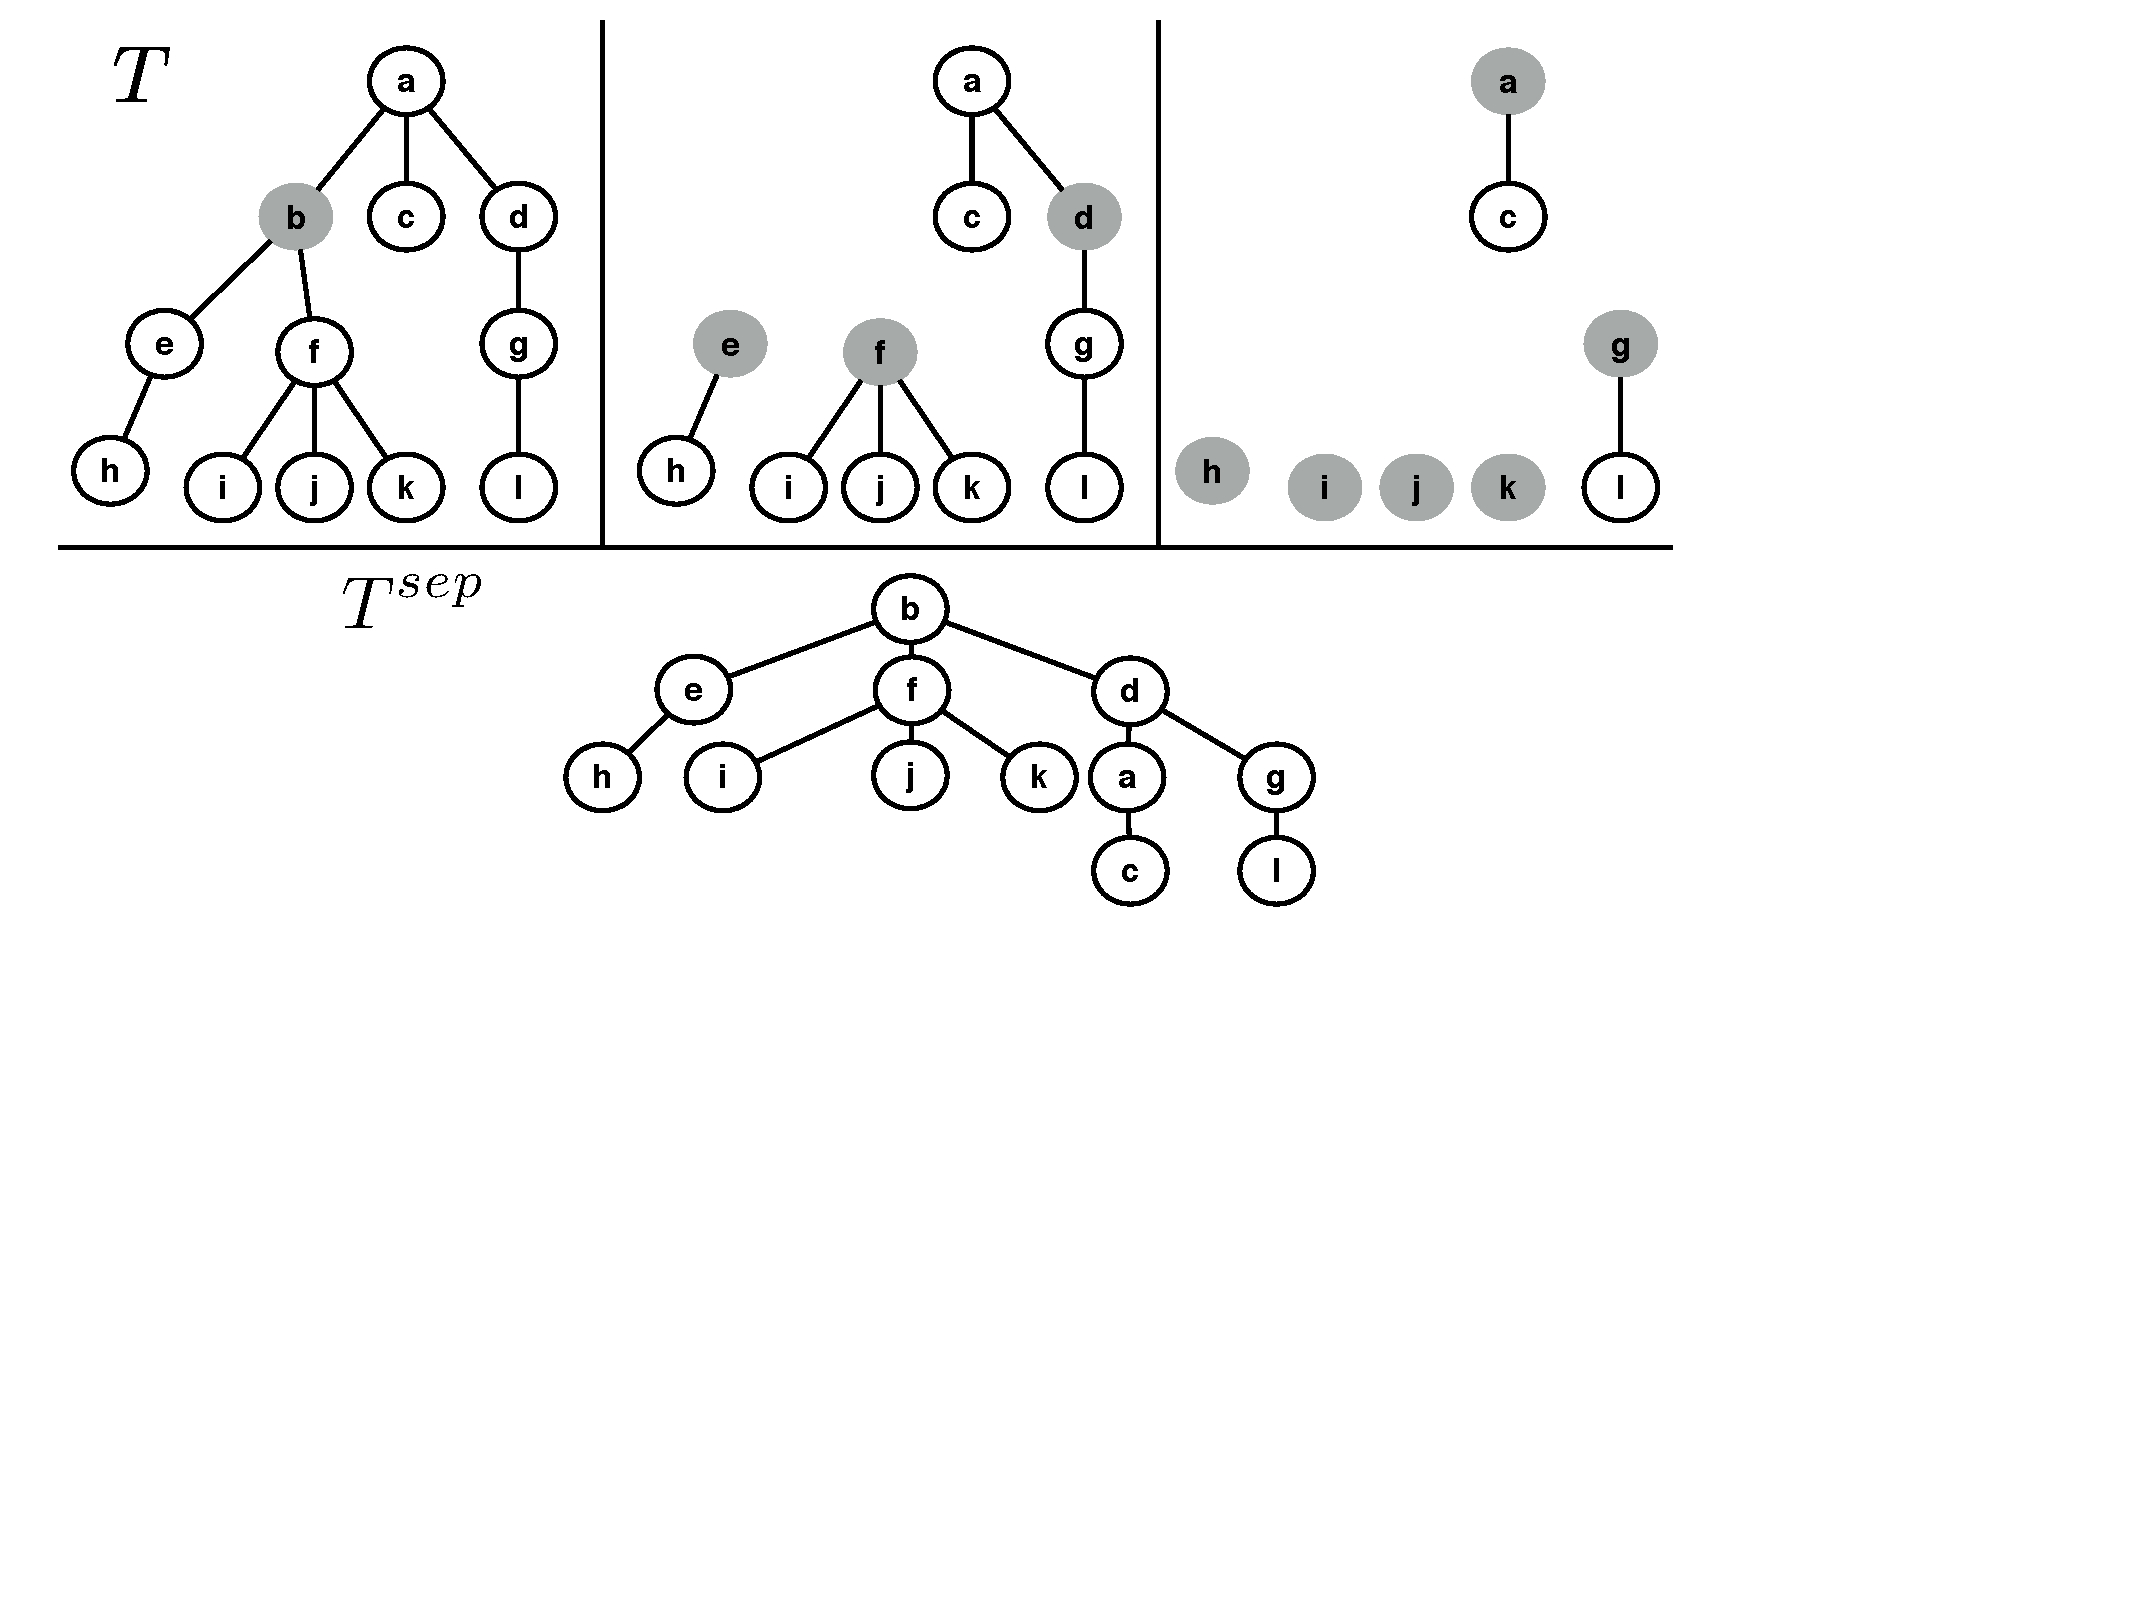
\includegraphics[width=80mm]{./Figures/Separator.pdf}
				\caption{Separator tree  for  the tree  $T$, with separator nodes marked  in grey. Top row:  $T$ rooted at $a$ (left). The forest resulted by removing the separator $b$ from  $T$ (center).  The remaining  forest after removing the  separators $e,f,d$ (right). Bottom row: the resulting $T^{sep}$. }
				\label{fig:separator}
			\end{figure}
			

 
\subsubsection{Spines decomposition}\label{tec:Splines}
This path-decomposition was invented by \citeN{Thorup01}, and used by \citeN{Korman10}.
Similarly to heavy-light decomposition, a \emph{spines decomposition}  decomposes an $n$ node tree $T$  into  a collection of paths, using an additional parameter, an integer $1 \leq b \leq n$.
A node $v$ is $heavy_{s}$ if $size(v) \geq n/b$ and $light_{s}$ otherwise. \todo{Is this standard terminology? It seems a bit weird to me...}
Note that the heavy nodes in $T$ induce a subtree rooted by the root of $T$, which is always  a $heavy_{s}$ node.
$T_h$ is the subtree of $T$ which spans the heavy nodes, and we note that  $T_h$ has at most $b$ leaves.
We  create a path-decomposition of $T_h$  by removing  every edge $(u,v)$ where $u$ has more than one child in $T_h$.
 This results in at most  $2b-1$ paths  $P_1 \dots P_l$, ($1 \leq l \leq 2b-1$) which  we denote as  $heavy_{s}$ paths (some of which may consist of a single node). When $b=2$, the  single $heavy_{s}$  path is referred  to  as the \emph{ spine} of $T$.

The spines decomposition of $T$ is  constructed recursively for subtrees in the forest $T \setminus T_h$ by using the above path-decomposition. 
The removal of $T_h$ from $T$ results in a forest $F$.
Note that a $light_{s}$ node $v$ in $T$ adjacent to a node in $T_h$ is  a root of a tree $T_v \in F$ of size $\size(v) \leq n/b$.
The decomposition stops when all nodes in $T$ are  $heavy_{s}$ nodes at some recursive step, and both node and path are of  \emph{level} $i$ if they occur at step $i$ in the decomposition.
Using  arguments similar to those for heavy-light decomposition, it follows that within at most $\log_{b} n$  steps all nodes in $T$ are $heavy_{s}$ nodes. 
See Figure~\ref{fig:ladder} for a demonstration.

				\begin{figure}[!ht]
				\centering
				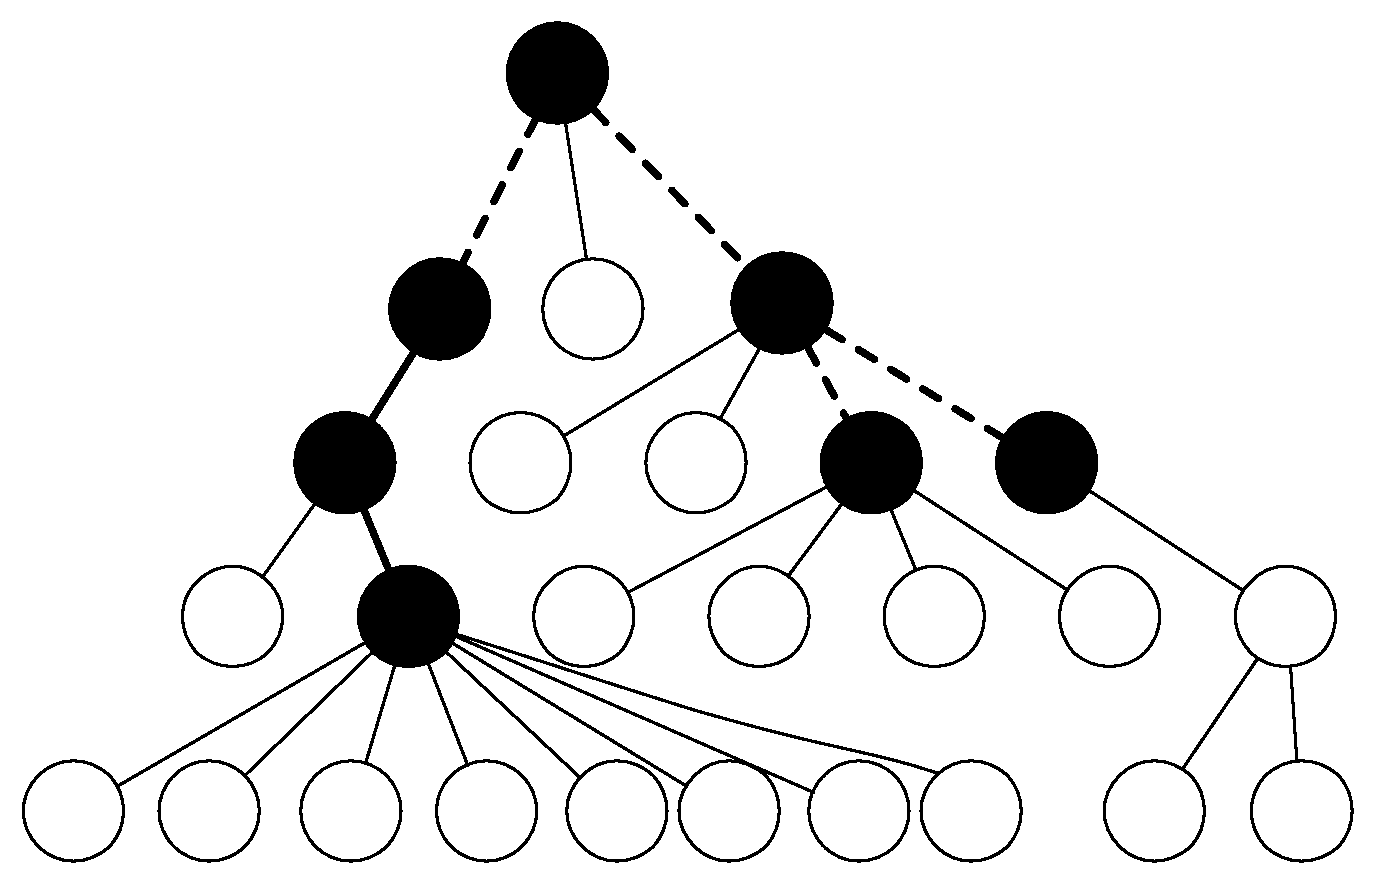
\includegraphics[width=50mm]{./Figures/Ladder_decomp.pdf}
				\caption{The first step of a  spines decomposition  of $T$ with $b=6$ for a tree with $n=24$ nodes. Black nodes are $heavy_s$ nodes, and the rest are $light_s$ nodes for the first step. Hatched lines are removed from $T_h$  and the emphasised edges mark the $heavy_s$ paths.}
				\label{fig:ladder}
			\end{figure}
			 

\subsubsection{Clustering}\label{tec:clustering}
The following  definitions are used to prove  that, given a number $x$ between $1$ and $n$, every tree can be decomposed into at most $n/x$ clusters with $O(x)$ nodes each, such that every cluster has at most two nodes in common with other clusters.

\begin{definition} \label{dfn:cluster}
Let $T$ be a tree of size $n = \vert V(T) \vert >1$.
 For a connected subtree $C$ of $T$, we call a node in $V(C)$ incident with a node in $V(T) \setminus V(C)$ a \emph{boundary node}.
The boundary nodes of $C$ are denoted by $\delta C$. 
A \emph{cluster} is a connected subtree of $T$ where $\vert \delta C \vert \leq 2$.
We denote $C(u,v)$ a cluster with the boundary nodes $u$ and $v$, where $depth(u)< depth(v)$.
If a cluster has only one boundary node, we associate  its rightmost leaf\footnote{The rightmost leaf of a tree $T$ is the last leaf encountered in the $\dfs$ traversal (see Section~\ref{tec:dfs}) of $T$.}  as the second boundary node.
Such clusters are called \emph{leaf} clusters. The remaining clusters are called \emph{internal} clusters.
 A set of clusters $\cs$ is a \emph{cluster partition} of a tree $T$ with root $r$ if and only if $V(T) = \cup_{C \in \cs}V(C)$, $E(T)= \cup_{C \in \cs} E(C) $, and for any distinct $C_1,C_2 \in \cs$, $E(C_1) \cap E(C_2) = \emptyset$, $\vert E(C_1) \vert \geq 1$, and $ r \in V(C)$ if $r \in \delta C$. \todo{The latter is unclear to me: doesn't this always hold for all nodes by definintion?}
\end{definition}

				\begin{figure}[!ht]
				\centering
				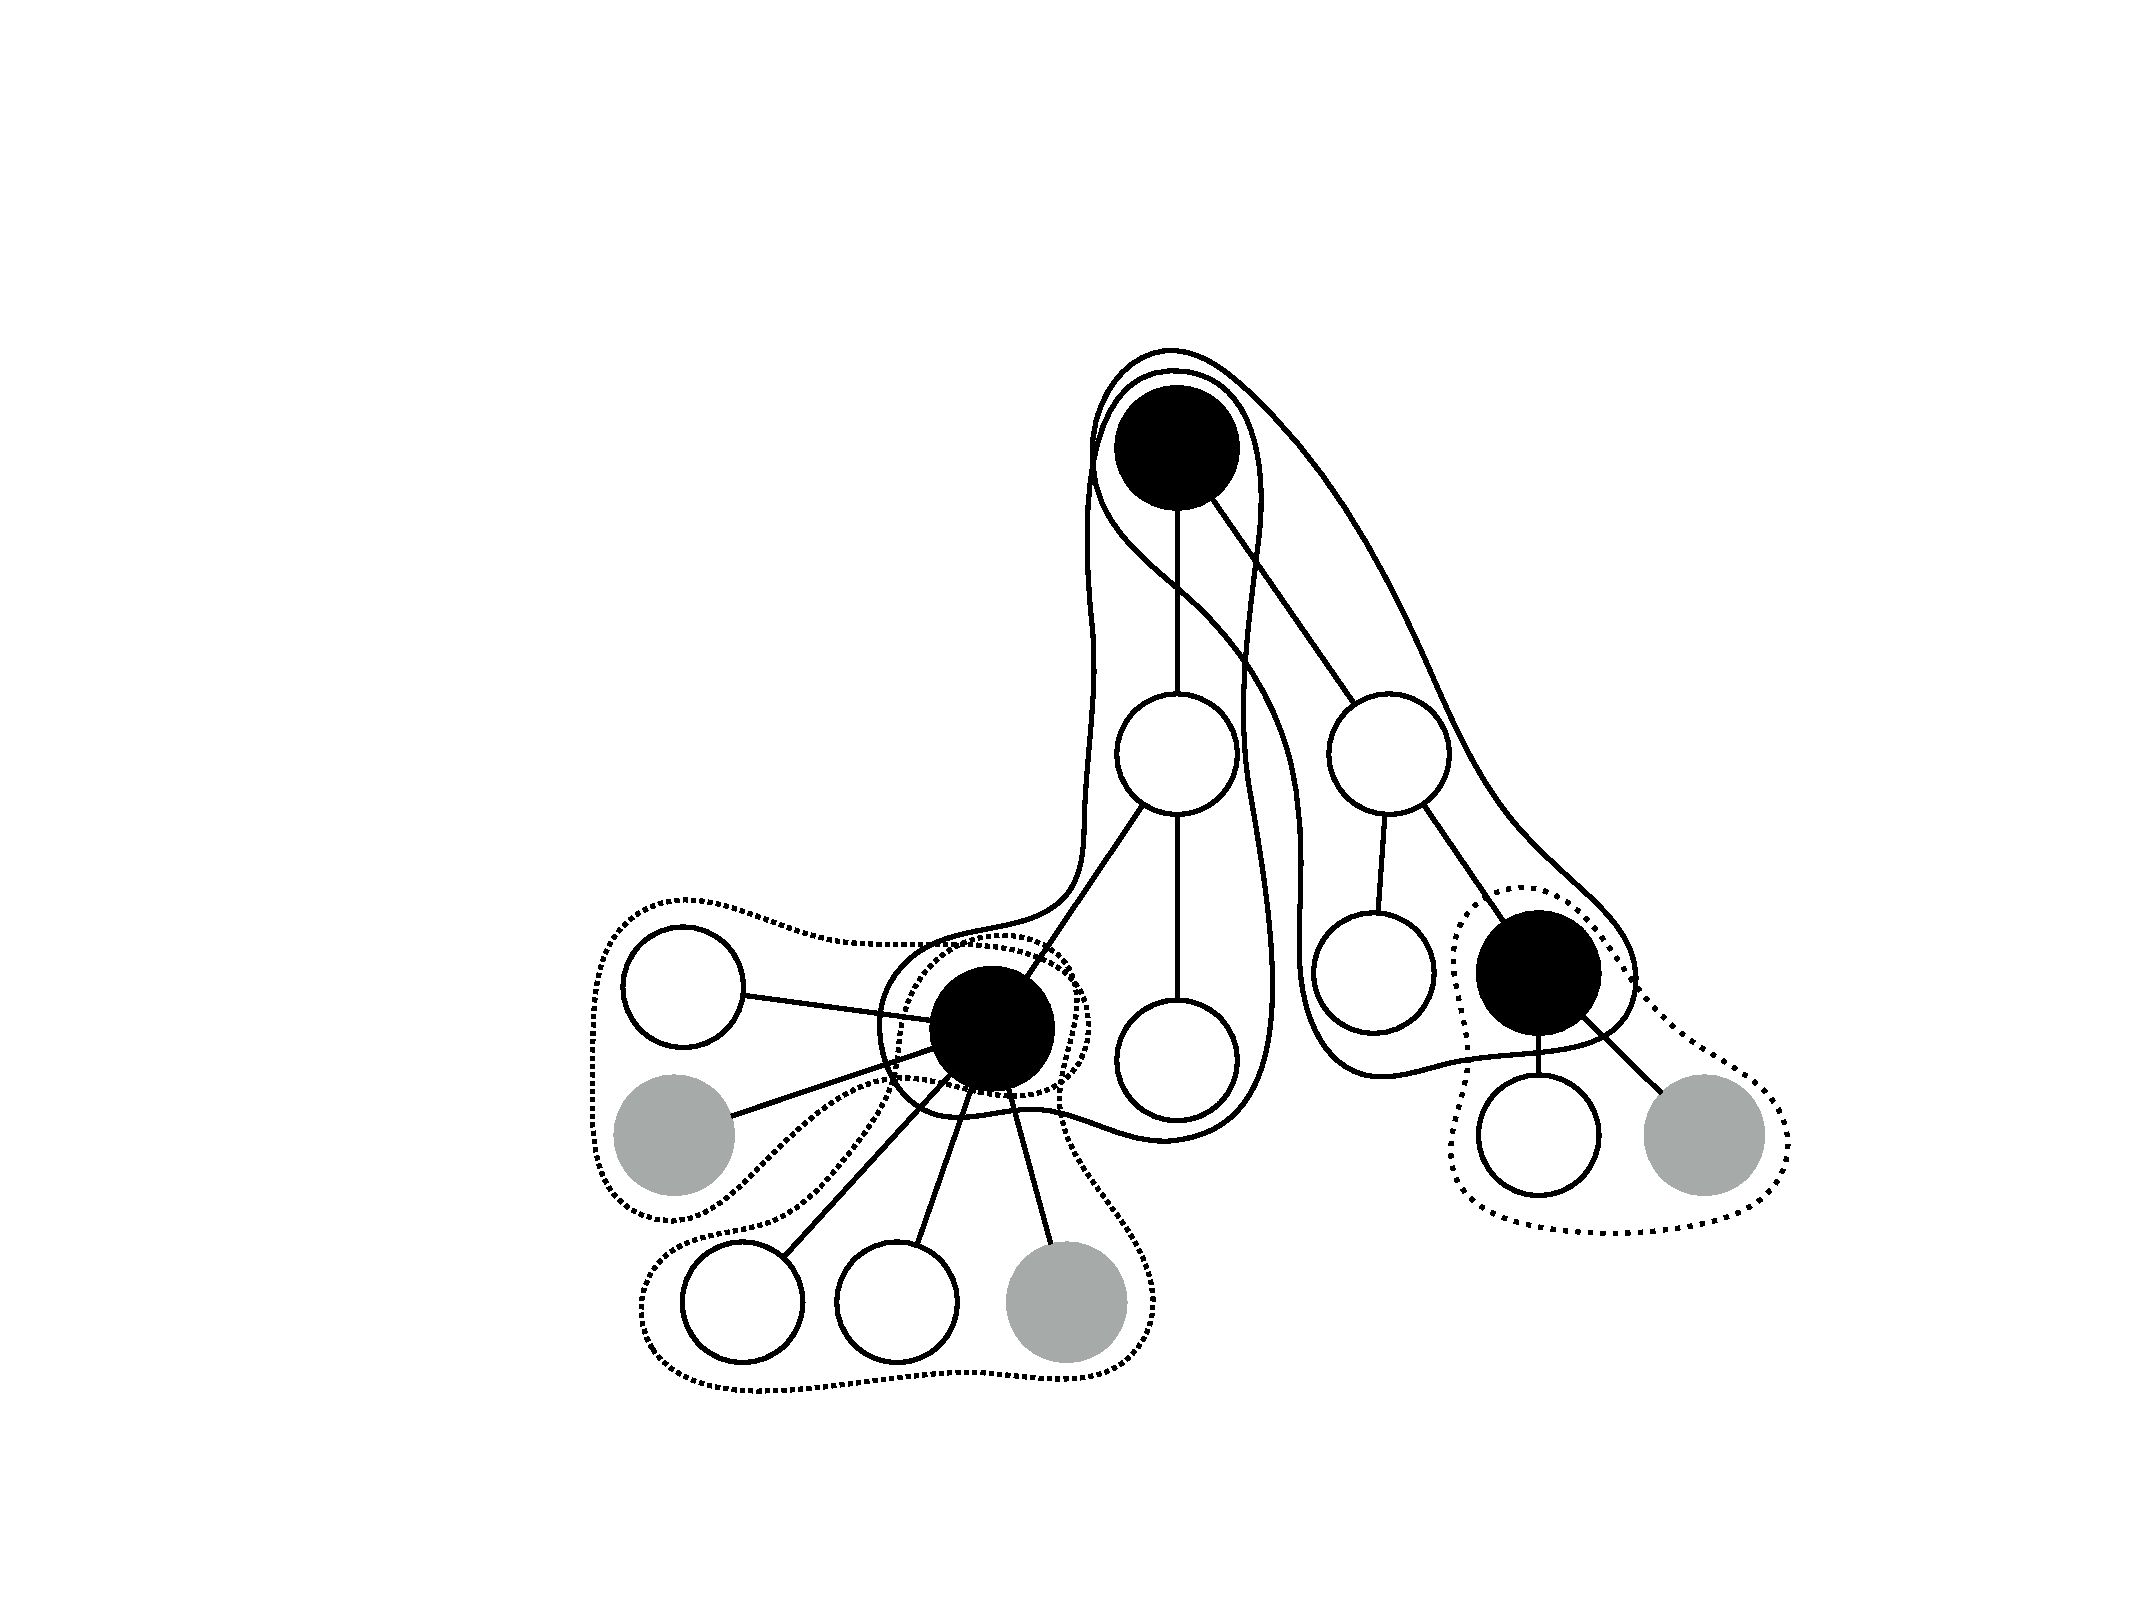
\includegraphics[width=40mm]{./Figures/newclustering.pdf}
				\caption{A demonstration of a nice cluster partition with $n=14$ and $x=4$. The dotted clusters are leaf clusters and the rest are internal clusters. The black nodes are boundary nodes, and the grey nodes  are the second boundary nodes added.}
				\label{fig:niceClusterDemo}
			\end{figure}
			
\begin{definition}\label{dfn:nice-cluster-partition}
Given a tree $T$ with $n>1$ nodes rooted at $r$ and a parameter $ 1 \leq x \leq n$. A cluster partition $\cs$ is a \emph{nice cluster partition}  if   $\vert \cs \vert \leq n/x$  and  $\vert V(C) \vert \leq cx$ for all $C \in \cs$, for some constant $c$. 
\todo{Shouldn't this definition depend on x? As in ``x-nice''?}
\end{definition}


\begin{lemma}\label{lemma:decomposition}
For any tree $T$ with $n$ nodes and any  $1 \leq x \leq n$ there exist a nice cluster partition. Moreover, such a partition can be computed in linear time.
\end{lemma}
A proof for the lemma can be found in \cite{alstrup1997finding} (Lemma 12, Appendix A), and an illustration of the decomposition in Figure~\ref{fig:niceClusterDemo}.
\todo{I think it is more than fair that we do not prove things here but just refer. But why do we then prove SOME things?}

\subsection{Boxes and groups}\label{section:boxes-and-groups}

This section presents a single lemma, which is used throughout the survey to prove lower bounds on label sizes. Introduced by Alstrup, Bille and Rauhe~\shortcite{Alstrup05} and refined  by \citeN{dahlgaard2014dynamic}. The technique uses a division  into ``boxes and groups'' of the set that is to be labeled.  

\begin{lemma}\label{lemma:boxgroups}
Let $X$ be a set with $|X|=nk$, where $n$ is a power of $3$ and $k\leq \log_3 n$. Further, let $e\colon X\to S$ be a function that labels the elements from $X$ with labels from some set $S$. Assume that we have partitioned $X$ into $k+1$ disjoint subsets of the same size:
\todo{Should $X$ have size $(k+1)n$ then?}
\[
X=X_0\cup\cdots \cup X_k, \quad \text{where $|X_i|=n$},
\]
and that we have further partitioned $X_i$ into  $3^i$  partitions of size $n/3^i$:
\[
X_i = X_{1,i}\cup\cdots\cup X_{n/3^i,i}, \quad \text{where $|X_{ij}|=3^i$.}
\]
We call each $X_i$ a \emph{box} and each $X_{i,j}$ a \emph{group}. Now, suppose that the following two conditions hold:
\begin{enumerate}[\normalfont (i)]
\item \label{item:boxgroup1} Two distinct elements of the same box have distinct labels.
\item \label{item:boxgroup2} If $x_1,x_2,x_1',x_2'\in X$ are elements such that $e(x_1)=e(x_1')$, $e(x_2)=e(x_2')$ and $x_1,x_2$ belong to two different groups in the same box, then $x_1',x_2'$ belong to two different groups.
\end{enumerate}
Then $|S|\geq n+(n/3)k$.
\end{lemma}
\begin{proof}
We show the claim by induction on $b \leq k$. \todo{What is b? Don't you mean k?}
For $b=0$,  by property~\eqref{item:boxgroup1}  each  of the elements in $X_0$ must have a  distinct label.
Assume that the claim holds for $b-1$.
Let $X_{prior}$ be the set of all boxes $X_0 \cup \cdots \cup X_{b-1}$.
We  show that the number of  elements in $X_{prior} \cup X_b$ sharing a label is at most $2n/3$:
 By property~\eqref{item:boxgroup1},  the labels assigned to $X_b$ are distinct.
The number of groups in $X_{prior}$ is $\sum_{i=0}^{b-1} 3^i < 2 \cdot 3^{b-1}$, and the number of groups in $X_b$ is $3 \cdot 3^{b-1}$.
From property~\eqref{item:boxgroup2} it follows that there are at least $(3-2)\cdot 3^{b-1}$ groups in $X_b$, each of size $n/3^b$ which may not share any element with $X_{prior}$, and thus, box $X_b$ contains at least $3^{b-1} n/3^b = n/3$ items of labels distinct in $X_{prior}\cup X_b$. 
\end{proof}




% Bibliography


\section{\ancestry}\label{section:Anc}
% !TEX root = ../Survey.tex
	We discuss labeling schemes for \ancestry.
	First, we describe  a simple $2 \log n$ labeling scheme for the function, followed by literature review in Section~\ref{sec:anc-lit}.
	We then present a recent labeling scheme  of size $\log n + 2\log \log n$ in Section~\ref{subsetion:mat-optimal}.
	The bound is matched  asymptotically by a  lower bound, presented in Section~\ref{sub-anc-lower}.
	Finally, in Section~\ref{sub-anc-dynamic}, we  discuss dynamic \ancestry labeling schemes and present in detail a lower bound for a natural dynamic model.

		\paragraph{Na\"ive algorithm}\label{section:NaiveAncestry}
		The following $2 \log n $ \ancestry labeling scheme was introduced by \citeN{Kannan92}.
		Similarly to the one in Section~\ref{sec:example}, it is composed of  two numbers in the set $\{1 \dots n\}$.
		Using a $\dfs$ traversal (Section~\ref{sec:efficient-encoding}), the encoder assigns   node $v \in T$, with  $ \la(v) =  (\dfs(v),\dfs(w))$ where $w$ is the descendant of $u$ with largest $\dfs$ number  (if $v$ is a leaf we set $w=v$).
		 
		Encoding each label is done in a single $\dfs$ traversal.
		The resulting label $\la(v)=(\dfs(v),\dfs(w))$  represents an interval $I(v)$, where  $I(r) =  \{1 \dots n\}$.
		Given the labels $\la(u)$ and $\la(v)$ the decoder  returns true if  $I(v) \subseteq I(u)$.
		 See Figure~\ref{fig:simple-ancestry} for a demonstration of the labeling scheme.
			  
			  
\begin{figure}[!ht]
\centering
\begin{tikzpicture}[scale=0.7,inner sep=0pt, minimum size=5ex, sibling distance=0.4em]
\tikzstyle{every node}=[draw,circle]
\Tree  [ 
.{1,23} 
	\edge; [.{2,11} [.{3,10} \edge[]; [.{4,5} \node{5}; ]
							       [.\node{6,8}; \node{7}; \edge; {8} ]
                       					       \edge; [.{9,10} \node{10}; ]
					    ] 
					    \edge; {11} ]
	\edge;  [.{12,13} \node{13}; ]
	[.\node{14,23}; \edge; {15}
			[.\node{16,22}; \edge; {17}
					[.\node{18,21}; \edge; {19}
							\node{20};
							\edge; {21} ]
					\edge; {22} ]
			\edge; {23} ]
	]
\end{tikzpicture}
\caption{
A tree with $n=23$ nodes. Each node is assigned a label of size $2 \log n$ supporting \ancestry queries.} \label{fig:simple-ancestry}
\end{figure}
			
			
\subsection{Literature review}\label{sec:anc-lit}
	\ancestry  labeling schemes are typically classified into two categories; \emph{range-based} and \emph{prefix-based}.
	  \emph{Range-based} labels, such as the na\"ive labeling scheme, are decoded by  comparing the  ranges assigned to each node. An additional example of a range-based  labeling scheme is found in Section~\ref{subsetion:mat-optimal}.
	 \emph{Prefix-based} labels are decoded by comparing the prefix of both labels such that $u$ is an ancestor of $v$ if and only if $\la(u)$ is  a prefix of $\la(v)$.
	 An example of prefix-based labeling scheme is found in Section~\ref{sub-anc-dynamic}.
	  
	The $2\log n$ labeling  scheme presented above was improved gradually.
	 Abiteboul, Kaplan and Milo \shortcite{Kaplan01} achieved an upper bound of  $3/2 \log n +O(\log \log n)$ bits, which was improved  to $\log n + O(\sqrt{\log n})$~\cite{Alstrup06}.
	 Shortly after,  Alstrup and Bille \shortcite{Alstrup05} constructed a lower bound of $ \log n + \log \log n$ for any labeling scheme supporting the function.
	\citeN{Fraigniaud10} showed that $Trees(n, \delta)$ enjoy a labeling scheme of $ \log n+ O(\log \delta)$.
	The result was  generalised in a follow up paper~\cite{Korman10} for $Trees(n)$ in a labeling scheme of size $\log n+ 4 \log \log n $, which is asymptotically optimal. The bound was improved last by~\citeN{knudsen2014private} to $\log n + 2 \log \log n$.
	 Interestingly, the asymptotically optimal  labeling scheme  is based on  the first one presented eighteen years prior \cite{Kannan92}.
	
	In the case where \ancestry may be determined if the distance between the nodes is at most $d$, \citeN{Alstrup05} constructed a labeling scheme
	 of size $\log n + O( d \sqrt{ \log n})$, for which the new upper bound performs better for any $d$.
	 
	 Due to their great applicability in queries for XML documents, a staggering number of papers address this practical aspect~\cite{kaplan2002comparison,wu2004prime,o2004ordpaths,li2005qed,lu2005region,harder2007node,harder2007node,xu2009dde,cohen2010labeling,o2012scooter,ghaleb2013novel}.
	 Typically, those address the dynamic variant thereof.  For a short survey on  dynamic \ancestry labeling schemes, see~\cite{cohen2010labeling}.
	 
\subsection{Upper bound} \label{subsetion:mat-optimal}
In this section we prove the following.
  \begin{theorem}
  There exist a $\log n + 2\log \log n + O(1)$ \ancestry labeling scheme for $Trees(n)$.
  \end{theorem}
  
The  na\"ive labeling scheme presented above stores a two part label  $(x_v,y_v)$ for every node $v$ in a tree $T$ that represent the  interval $\{x_v \dots y_v\}$ of size $y_v-x_v+1$. Both  $x_v$ and $y_v$ may be any number in  $\{1 \dots n\}$ and therefore the label size is at most $2\log n$. The label  can also be stored in the form $(x_v,y_v-x_v+1)$ as demonstrated by the following pseudo code. 
The function computes a value $a$   for every node $v \in T$ specifying the largest $x_{v'}$ for any $v'$  in the subtree rooted in $v$. 
The function is initially called on  the root $r$  of $T$ and $\Id= 1$. 

\begin{algorithmic}[1] \Function{na\"ive}{node $v$, integer $\Id$}
        \State $a \gets \Id$	
	\ForAll{$l \in \children(v)$}   
	\State $a \gets  \Call{na\"ive}{l,a+1}$ 
	\EndFor
	\State $v.label \gets (\Id,(a-\Id))$ 
	\State \Return $a$  
\EndFunction
\end{algorithmic}


To reduce the label size further, we do not store $y_v-x_v+1$ explicitly. 
Instead, we use  an approximation  of that value that  requires only $O(\log \log n)$ bits. 
The value $x_v$ is now computed using an updated variant of the $\dfsi$ traversal (Section~\ref{sec:efficient-encoding}).
In particular, the order of the traversal remains the same.
While $x_v \geq \dfsi(v)$, it will  still hold that $x_v = O(n)$.

 As described in  Section~\ref{section:Misc-Tools}, we can store a $1+\frac{1}{2^k}$ approximation of any number in the range $\{1 \dots n\}$ using   $\log  \log n + k$ bits. The following labeling scheme uses $1+\frac{1}{2^k}$ approximation for carefully  chosen $k$.  For brevity, we now  denote $\frac{1}{2^k}$ by  $\epsilon$, and call $\app(x)$ the function that returns a $1+\epsilon$ approximation of an integer $x$.
Notice that  $ \log \log  x + \log\frac{1}{\epsilon}$ bits are required  to store the result of the function.

The label of a node $v$ in a rooted tree $T$ consists of the following two parts  $\la(v) = (\Id(v), \Ap(v))$.
For every node $v \in T$ the function \textsc{improved}  computes  two values, $a$ and $b$: in this $a$ stands for the largest number assigned and $b$ the largest number reserved  in the subtree rooted in $v$.
We initially call the  recursive  function using  the root of $T$ and $\Id = 1$. 

\begin{algorithmic}[1] \Function{improved}{node $v$, integer $\Id$}
        \State $(a,b) \gets (\Id,\Id)$	
	\ForAll{$l \in \children(v)$ in   increasing ordered size}   
	\State $(a,b) \gets  \Call{improved}{l,b+1}$ 
	\EndFor
	\State $v.label \gets (\Id,\app(a-\Id))$ 
	\State \Return $(a,\max{ \{b,\app(a-\Id)+\Id\}})$  \label{line:critical}
\EndFunction
\end{algorithmic}
   To prove that the encoder assigns labels of the requested size we first use  lemma~\ref{Lemma:newwriting}.
Recall  that $\ldepth(v)$ is the number of light nodes encountered on the path $r \leadsto v$, and that  the  $\ldepth(T)$ is the maximum light depth among the nodes in the tree $T$ (Section~\ref{tec:heavylight}). 
Recall also  that a node $v$ in a  tree $T$ roots the subtree $T(v)$ of size $\size(v)$.
\begin{lemma}\label{Lemma:newwriting}
Let $v$ be  a node in a tree $T$  of size $S = \size(v)$,   $x$ be an integer, and $l = \floor{\log S}$.
If $(a,b)=\textsc{improved}(v,x)$ then:
\begin{enumerate}
	\item $a \leq x + S(1+\epsilon)^l -1.$
	\item $b \leq x + S(1+\epsilon)^{l+1}-1.$
\end{enumerate}
\end{lemma}
\begin{proof}
		We prove the claims by induction over $l$, where the claims hold trivially for $l =1$.
		Assume that both claims hold for $l-1$  and we show that it holds for $l$.
		The children of $v$ are denoted $w_1 \dots w_k$ according to their size, where $w_k$ is the heavy node.
		The $a$ and $b$ values of  node $w_i$ are called $a_i$ and $b_i$ respectively.
		Since $w_1 \dots w_{k-1}$ are light nodes, $\size(w_1) \dots \size(w_{k-1}) < \frac{1}{2}S$, which implies that  $\floor{\log \size(w_i)} \leq l-1$.
		Thus, by the induction hypothesis  $b_1 \leq  x + \size(w_1)(1+\epsilon)^{l}-1$. 
		For both manners of  assigning $b_2$ (line~\ref{line:critical}) it now holds that,  
		$$b_2 \leq  b_1+1 + \size(w_2)(1+\epsilon)^{l}-1 \leq  X + (\size(w_1)+\size(w_2)) (1+\epsilon)^{l}-1.$$
		Applying the argument to all $b_i$ $3 \leq i \leq k-1$ we get:
		 $$b_{k-1} \leq   x +  \sum_{i=1}^{k-1}\size(w_i) (1+\epsilon)^{l}-1$$
	At this point  we can use the first hypothesis to get:
	$$a_{k} \leq  x +  \sum_{i=1}^{k-1}\size(w_i) (1+\epsilon)^{l} + \size(w_k)(1+\epsilon)^l$$
	Which is simply $S(1+\epsilon)^l-1$ As requested. The proof of the second argument is done similarly.
	\end{proof}
 
Since $l = \floor{\log S} \leq \log n$, by Lemma~\ref{Lemma:newwriting} the  total interval required is of size at most $\floor{n \cdot (1+ \epsilon)^{\log n}}$.
  It follows that the size of the first label part is at most $ \log n +  \log n \cdot \log(1+ \epsilon)+O(1)$ and the size of the second part is at most $\log \log  n + \log\frac{1}{\epsilon}+O(1)$. Choosing $\epsilon = 1/ \log n$, these are bounded by $\log n + O(1)$ and   $2 \log \log n+O(1)$, respectively.
  
 The encoding is done similarly  to the na\"ive decoder.
  Given labels $(\Id(v),\Ap(v))$ and $(\Id(u),\Ap(u))$ of nodes $v$ and $u$, respectively, the node  $v$ is an ancestor of $u$ if and only if $\Id(v) \leq \Id(u) \leq \Id(v)+(1+\epsilon)^{\Ap(v)}$. 
 In this labeling scheme the interval of a node's  decedent  may be of equal size to the one used by the node. Therefore, unlike the na\"ive labeling scheme, the intervals are not necessarily  fully contained. 
 	
\subsection{Lower bound}\label{sub-anc-lower}
The following  lower bound is an extension of the one by \citeN{Alstrup05} using the same technique, namely, boxes and groups (Section~\ref{section:boxes-and-groups}). 
\begin{theorem} \label{theo:ancestrytreeslower}
For any $n,\delta$ with $n\geq \delta+1\geq 3$, any \ancestry labeling scheme for $Trees(n,\delta)$
has a worst-case label size of at least $\ceil{\log n} + \floor{\log \floor{\log \delta}}-1$.\footnote{Observe that the assumption $n\geq \delta+1$ is natural, since any tree with $n$ nodes and depth $\delta$ satisfies $n\geq \delta+1$.}
\end{theorem}
\begin{proof}
Let $m=2^{\floor{\log (n-1)}}=2^{\ceil{\log n}-1}$ be $n-1$ rounded down to the nearest power of $2$, and set $k=\floor{\log \delta}$. Note that $k\leq \log m$. Construct for $i=1\dots k$ the tree $T_i$ as a root node to which $m/2^i$ paths of length $2^i$ have been attached. Thus, $T_i$ has $m+1\leq n$ nodes, whereof $m$ belong to disjoint paths. Further, $T_i$ has depth $2^i\leq 2^k\leq \delta$, and hence $T_i$ belongs to $Trees(n,\delta)$. For an illustration of such trees see Figure~\ref{fig:TheosDrawing}.

Each node in a tree must be uniquely labeled by an \ancestry labeling scheme. Further, if two nodes in $T_i$ lie on distinct paths, then their labels cannot be used on the same path in $T_j$ for any  $j\neq i$, because nodes on the same path have an \ancestry relation whereas nodes on different paths do not. We can therefore apply Lemma~\ref{lemma:boxgroups}, using the $m$ nodes of the paths of each tree as a ``box'' and each path as a ``group'', and it follows that we need at least $\frac{1}{2}m(k+1) = \frac{1}{2}m(\floor{\log \delta}+1)$ labels. If the worst-case label size is $L$  we can create $2^{L+1}-1$ distinct labels, and we must therefore have $\frac{1}{2}m(\floor{\log \delta}+1)\leq 2^{L+1}-1$ from which it follows that $L\geq \ceil{\log n} + \floor{\log \floor{\log \delta}}-1$.
\end{proof}
			
			\begin{figure}[!ht] 
				\centering
				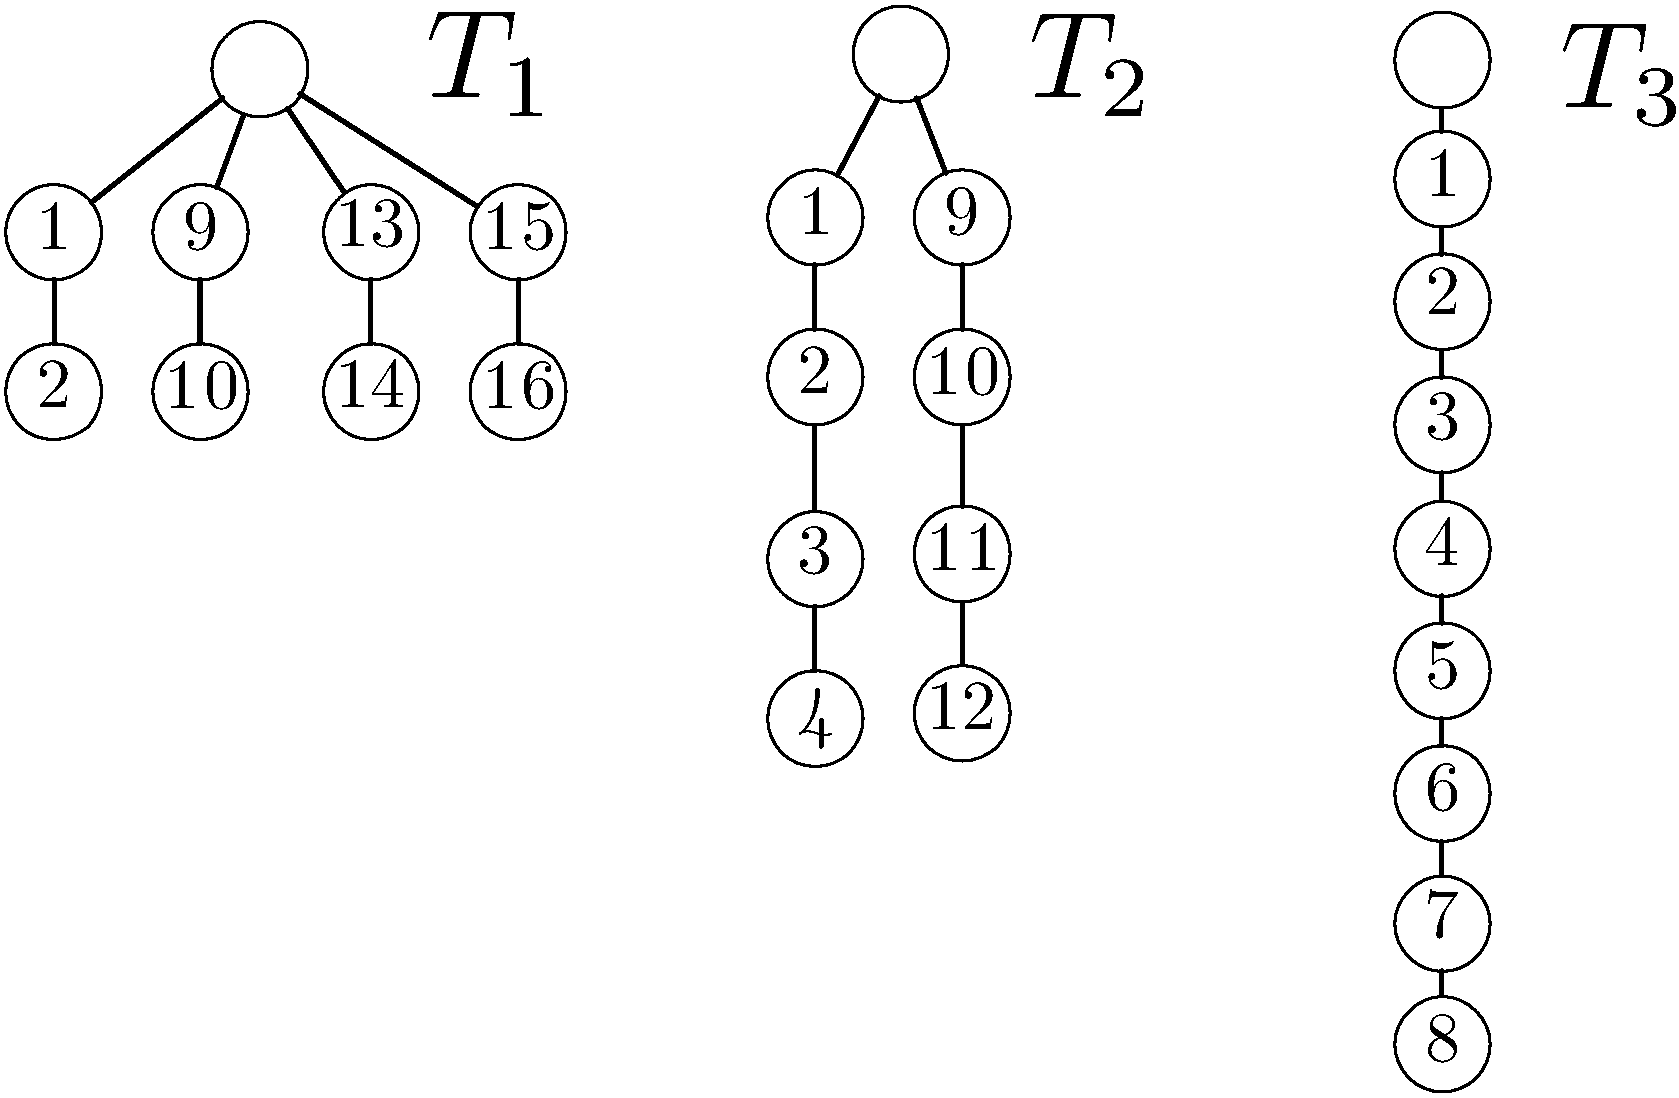
\includegraphics[width=60mm]{./Figures/Lowerbound-ancestry.pdf}
				\caption{Illustration of $T_1,T_2,T_3$ for $n=8$. }
				\label{fig:TheosDrawing}
			\end{figure}

%\subsection{Siblings and connectivity} \label{section:Sib}
%The lower bound presented above can be derived for the functions Siblings and connectivity.
%In contrast to ancestry, attaining a $\log n + \log \log n$ labeling scheme for both functions is easy.
%Moreover, if the labels are not necessarily unique, a straightforward $\log(n)$ labeling scheme exist for both.

\subsection{Dynamic \ancestry labeling schemes}	\label{sub-anc-dynamic}	
			All results described thus far in the survey present a worst-case analysis of static trees.
			We  describe the first dynamic result, in which rather than receiving a tree $T$, the decoder receives a sequence of $n$ operations constructing $T$.
			Operations considered in the literature are insertions  and deletions of leaves, or arbitrary nodes.
			For convenience  it is assumed that the sequence constructs a rooted tree, and its root exist from the beginning and  is never  deleted.
			
			The section discusses a  \emph{persistent} \ancestry labeling scheme, i.e a dynamic labeling scheme that does not change the label given to a node.
			The result is described in a model in which the operation allowed is an  insertion of  leaves.
			%For labeling schemes with permitted relabelling, as well as further implications of the result presented see Section~\ref{section:dynamic}.

			A trivial prefix-based labeling \ancestry labeling scheme for the model is  built directly from the suffix free  $code_0$ (Section~\ref{tec:suffix}).
			The root $r$ receives the label $1$. Suppose   node $v$ receives the label $\la(v)$. The $i$'th child of $v$ receives the label $\la(v) \circ 10^{i-1}$.
			Decoding $\la(u),\la(v)$ is done in the standard way, and the label size is at most $O(n)$.
			The next section proves that this trivial labeling scheme is asymptotically  optimal.
			
			\paragraph{Lower bound for persistent \ancestry labeling scheme}
			Cohen, Kaplan and Milo \shortcite{Cohen02} proved a lower bound of  $\Omega(n)$ on the label length for a sequence of $n+1$ insertions.
			They do so by presenting a family of insertion sequences of size $2^{n-1}$, such that each sequence has  at least one node with unique label.
			\begin{definition}\label{dfn:kaplans-trees}
			We define the family of insertion sequences $\mathcal{F}(n)$ recursively as follows.
				$\mathcal{F}(1)$ consists of a single sequence which inserts a root $r$ and a child of $r$, $w$.
				$\mathcal{F}(n)$ \textit{extends} each sequence $s$  in  $\mathcal{F}(n-1)$ rooted in $r$ to two sequences $s_1$ and $s_2$.
				Both insertion sequences replace the insertion of the root $r$ by the sequence $r'$ and $w'$,  a child of $r'$.
				$s_1$ is defined by connecting nodes previously adjacent to $r$  to be adjacent to  $w'$.
				In the same manner, $r'$ ``replaces'' $r$ in  $s_2$. 
				For illustration, see Figure~\ref{fig:KaplansTrees}.
			\end{definition}
			For convenience, we denote the last node in a sequence $s$, as $last(s)$, and the set of all sequences $s_2$, respectively~$s_1$ in $\mathcal{F}(n)$ created from $s \in \mathcal{F}(n-1)$ as  $s_2$ type sequence respectively~$s_1$ type sequence.	
			
			Since  $\vert \mathcal{F}(1) \vert = 1$, and  $\vert \mathcal{F}(i) \vert = 2 \cdot \vert \mathcal{F}(i-1) \vert $ it follows that the number of insertion sequences is $\vert \mathcal{F}(n) \vert = 2^{n-1}$.
			Each insertion sequence in $\mathcal{F}(n)$ has one more node than the sequence it was built upon from $\mathcal{F}(n-1)$. 
			Since the size of the sequence in $\mathcal{F}(1)$ is $2$, it follows that the size of each insertion sequence in $\mathcal{F}(n)$ is $n+1$.
			
			\begin{figure}[!ht] 
				\centering
				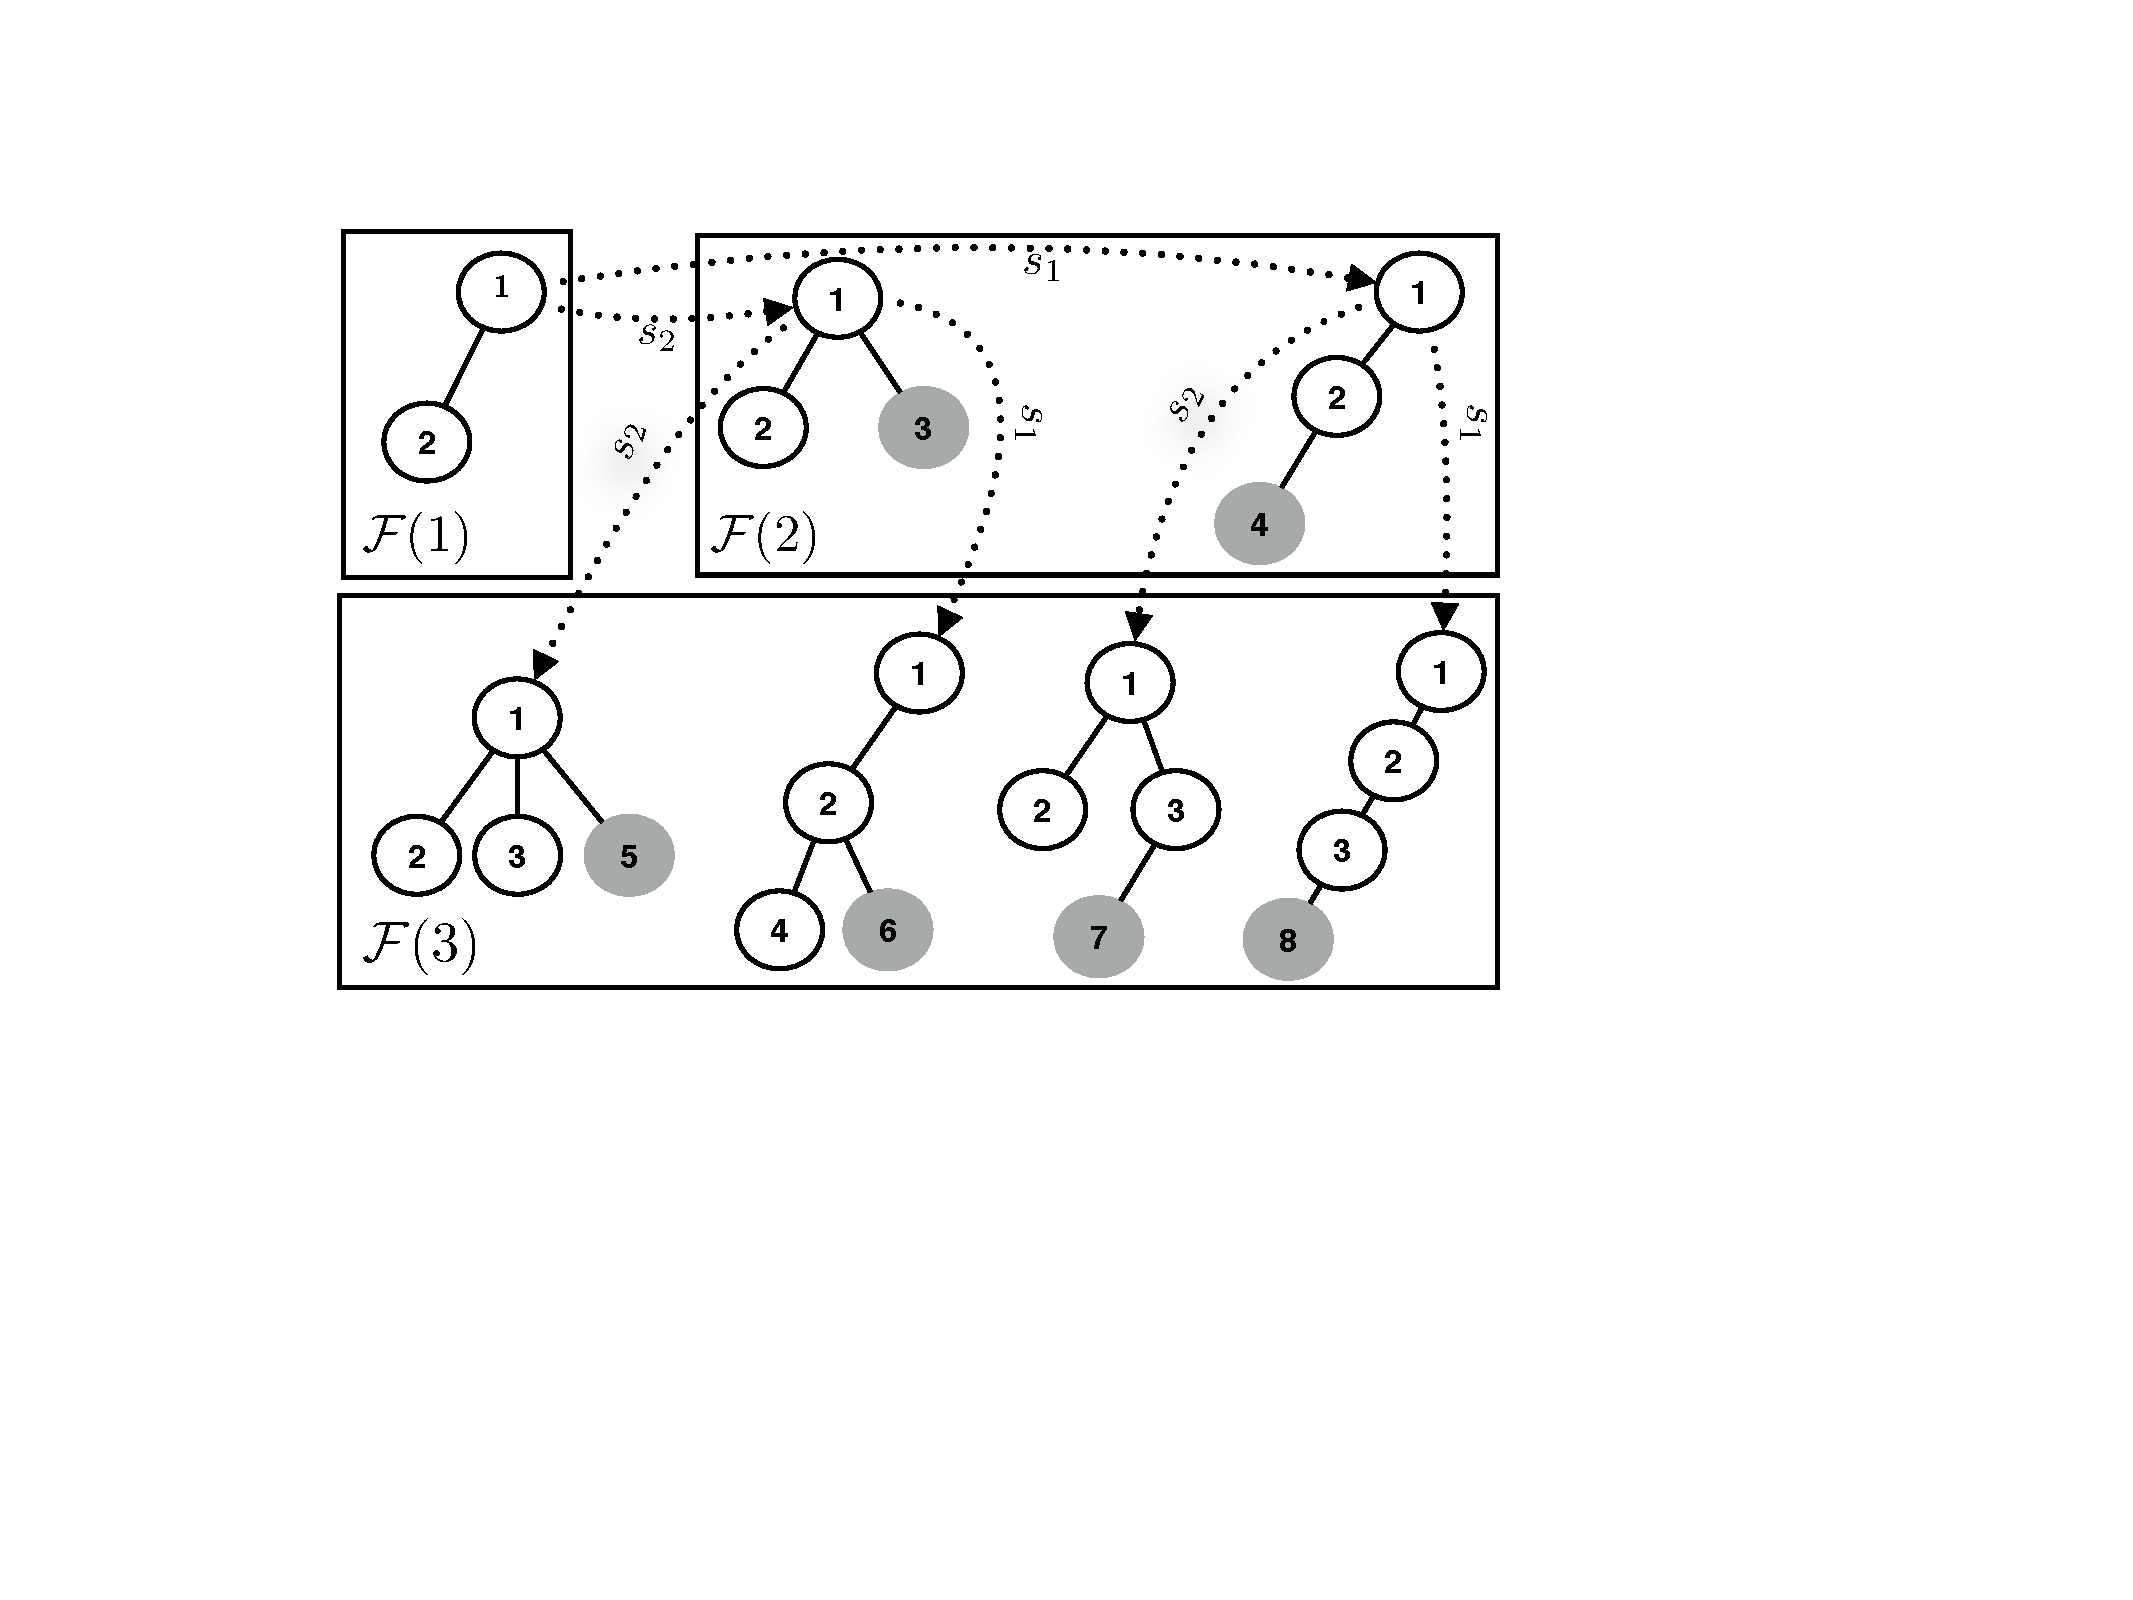
\includegraphics[width=70mm]{./Figures/Kaplans.pdf}
				\caption{ An illustration of  the trees resulting by the sequences $\mathcal{F}(1)$,  $\mathcal{F}(2)$ and  $\mathcal{F}(3)$ from Definition~\ref{dfn:kaplans-trees}. The grey nodes are the ones introduced by Lemma~\ref{lemma:persistent}.
				The arrows denote the extension of a sequence, and marked $s_1$ or $s_2$ according to the type.}
				\label{fig:KaplansTrees}
			\end{figure}
			
			We proceed to present the lower bound.
			\begin{lemma}\label{lemma:persistent}\cite{Kaplan01}
				Any  persistent  \ancestry labeling scheme with a deterministic encoder must give a unique label to the last insertion in  each of the  insertion sequences in $\mathcal{F}(n)$. 
			\end{lemma}

			\begin{proof}
				The claim is proved by induction.
				Suppose the claim is true for $\mathcal{F}(n-1)$, and pick two  insertion sequences $s, s' \in \mathcal{F}(n-1)$.
				 Denote the  sequences  extending  $s$ and $s'$ using  the first extension  type $s_1$ and $s'_1$ respectively.
				From the induction hypothesis it follows directly that $\la(last(s_1)) \neq \la(last(s_1'))$. %An illustration thereof is available in Fig.~\ref{fig:KaplansTrees}.
				
				Denote now both  derived sequences of $s$ in $\mathcal{F}(n)$ as  $s_1$ and $s_2$.
				Since the encoder is deterministic, and the first two elements of the insertions are identical,  $r'$ and $w'$ receives the same label in both.
				The node $last(s_1)$ is not a decedent of $w$ but $last(s_2)$ is.
				 Since the decoder needs to determine an \ancestry relation, $d(\la(w),\la(last(s_1))) = false$ and $d(\la(w),\la(last(s_2))) = true$.
				  Therefore, it is required that $\la(last(s_1)) \neq \la(last(s_2))$. 
			\end{proof}
				
				From Lemma~\ref{lemma:persistent}, and since there are $2^{n-1}$ insertion sequences of size $n$, it follows that $2^{n-1}$ distinct labels are needed for the last node in each sequence in $\mathcal{F}(n)$.
			\begin{corollary} \label{cor:persistent}
				Every persistent \ancestry labeling scheme  $\tuple{e,d}$ is of size $\Omega(n)$.
			\end{corollary}
			Using a similar argument, \citeN{Cohen02}  prove that the bound  holds for  a sequence corresponding to a tree from $Trees(n,\Delta)$, when $\Delta \geq 2$.
			Moreover, the bound is shown to hold even when the encoder is allowed to use randomisation.
			

		To overcome this inherent difficulty, the authors introduce the notion of \emph{sibling} and \emph{direct clues}.
			Loosely speaking, sibling, respectively, direct clues provide every node $v$ in the sequence a guarantee on the  range of possible number of $v$'s siblings, respectively~size of $v$.
		Using this method, they show tight bounds on the label sizes for such labeling schemes with  $\Theta(\log n)$ bits using sibling clues  and  $\Theta( \log^2 n)$ bits using direct clues. \citeN{dahlgaard2014dynamic} showed that this bound applies for the functions \NCA, \distance, and \routing as well. In contrast, they showed that $2 \log n$ are sufficient and necessary in this model for the functions \adjacency, \siblings and \connectivity.	
			


%% !TEX root = ../Survey.tex
\newpage
\section{Distance and related problems} \label{section:distance}
	The section begins in a rather broad literature review. 
	We then proceed to show the upper bound.
	A tight  connection between Distance, NCA in the fixed port model and separation level.
	We proceed by presenting  a revised lower bound.
	At this point we show results relating to approximate distance.
	After which we  show the dynamic labeling scheme by Korman.
	We finish the chapter by mentioning a close result of small distances in trees.
	
\subsection{Literature review}
	Distance labels were investigated at first by Peleg \cite{Peleg00}.
	Gavoille et al.~\cite{gavoillea2004distance,Gavoille2001} established a lower bound for $Trees(n)$.
		 Kano et. al~\cite{Kano07} present an average case analysis  for the function.
		Additional efforts by Kaplan \cite{Kaplan01} and Alstrup \cite{Alstrup05} showed a parameterized variant, where  the labeling scheme is limited to answer queries  up to some $k$. The first result presented a labeling scheme of  $\mathcal{O}(\log n + k \sqrt{\log n})$  \cite{Kaplan01}, and  improved  to $\log n+\mathcal{O}(k^2(\log \log n + \log k))$ \cite{Alstrup05}.	
		A well investigated variant are the approximate distance labeling schemes.
		Using $O(\log n \cdot \log \log n)$ bits Katz showed that an approximate scheme of $1+1 / log n$ stretch is possible.  The scheme still maintains distances for the separator at each level, using the first $\log \log n$ most significant bits \cite{Katz00} of each distance.The distance table of a tree with $n$ nodes can be distributed to each node, such that its label will contain all distances, which implies a labeling scheme of size $n \log n$.
		The immediate improvement is to store only the distance from each node to all its vertices on the path to the root. 
		The decoding will find the \emph{NCA} of both $u$ and $v$,$w$, and return $dist(u,w)+dist(v,w)$.
		Although better in practice, the maximum length of the labeling scheme remains $O(n \log n)$.
\subsection{Upper bound}
		The main question regarding the naive solution is, if there could be a smaller subset of distances to maintain in each label.
		For trees Peleg showed that it could be done with at most $\log n$ of those.
		Peleg considered  the weighted case with maximal weight $2^M$, and showed a  $O(M \log n + \log^2 n)$  distance labeling scheme, which yields a  $O(\log^2 n)$  distance labeling scheme for the unweighted case.		
		The result was re-discovered by Peleg as a private case of a graph separator related distance labeling scheme \cite{Gavoille2001}.
		
		\begin{lemma}\label{lemma:torwardsDistance}
		Given a tree $T=(V,E)$ with $n$ nodes, we can find a vertex $v \in V$ such that each of the $i$ connected components of $T \setminus v$ is a tree of size at most $\frac{n}{2}$.
		We denote vertex $v$ as the \emph{separator}  of $T$, and the components as $c_1 \dots c_i$ marked in a non decreasing order with respect to their size.
		\end{lemma}
		
		\begin{thm}\label{thm:distance-upper}
		There exist a distance labelling scheme for $Trees(n)$ with size at most $O(\log^2 n)$.
		\end{thm}
		\begin{notproof}
		Lemma~\ref{lemma:torwardsDistance} is  applied recursively such that it is guaranteed that after $\log n$ steps, each component consists of a single vertex.
		We denote for each $0 \leq j \leq \log n$  the $j$'th separator as $v_{s_j}$, and the components introduced as $c_1^j \dots c_i^j$.
		Each vertex is labeled by  a concatenation of $\log n$ tuples $ \tuple{d_j,c_i^j}, 0 \leq j \leq \log n $, where  $d_j$ is  the distance of the vertex from $v_{s_j}$.
		It can be shown that $\sum_{j=1}^{\log n}c_i^j=O(n)$, and since each $d_j=O(\log n)$ in the unweighted case,  the label size is $O(\log^2 n)$.
		The decoder finds the first uncommon connected component and returns the sum of distances from the separator thereof.
		\end{notproof}


\subsection{Lower bound for $Trees(n)$}
Gavoille et al.~\cite{gavoillea2004distance,Gavoille2001} establish a lower bound for $Trees(n)$ using a technique where they apply a distance labeling scheme to a special class of trees called $(h,M)$-trees. 
%proof has some errors and unclarities, which we shall try to fix in the following exposition. We shall later describe in more detail the problems with their proof.
\paragraph{$(h,M)$-trees}.
 For $h\geq 0$ and $M\geq 2$, an \emph{$(h,M)$-tree} is a binary tree that is constructed recursively as follows. 
 For $h=0$, the tree  a single node. For $h>0$, the tree consists of a path of length $M-x$ for some $0\leq x<M$ whose one end point is the root of the tree and whose other end point is the start node of two paths of length $x$ whose end points are the roots of two $(h-1,M)$-trees. An example for $h=3$ can be seen in  Fig.~\ref{fig:hMtree}.  We shall denote an $(h,M)$-tree constructed in this way by $T=\langle T_0,T_1,x\rangle$, where $T_0$ and $T_1$ are the two $(h-1,M)$-trees attached to the ends of the two paths of length $x$. Note that, if $x=0$, then the two paths of length $0$ collapse into a single node, and the two subtrees $T_0$ and $T_1$ are then both attached to this node.

\begin{figure}
	\centering
	\begin{tikzpicture}[sibling distance=3em, inner sep=0pt, minimum size=1ex]
	\tikzstyle{every node}=[draw,circle,fill=black]
	\Tree [.{} \edge node[draw=none,fill=none,auto=right] {$M-x$}; [.{} 
		\edge node[draw=none,fill=none,auto=right] {$x$}; [.{} \edge node[draw=none,fill=none,auto=right] {$M-y_1$}; [.{} 
			\edge node[draw=none,fill=none,auto=right] {$y_1$}; [.{} \edge node[draw=none,fill=none,draw=none,fill=none,auto=right] {$M-z_1$}; [.{} \edge node[draw=none,fill=none,auto=right,pos=.6] {$z_1$}; [ .{} ] \edge node[draw=none,fill=none,auto=left,pos=.6] {$z_1$}; [ .{} ] ] ]
			\edge node[draw=none,fill=none,auto=left] {$y_1$}; [.{} \edge node[draw=none,fill=none,auto=left] {$M-z_2$}; [.{} \edge node[draw=none,fill=none,auto=right,pos=.6] {$z_2$}; [ .{} ] \edge node[draw=none,fill=none,auto=left,pos=.6] {$z_2$}; [ .{} ] ] ]
			]
		]
		\edge node[draw=none,fill=none,auto=left] {$x$}; [.{}	\edge node[draw=none,fill=none,auto=left] {$M-y_2$}; [.{}
			\edge node[draw=none,fill=none,auto=right] {$y_2$}; [.{} \edge node[draw=none,fill=none,auto=right] {$M-z_3$}; [.{} \edge node[draw=none,fill=none,auto=right,pos=.6] {$z_3$}; [ .{} ] \edge node[draw=none,fill=none,auto=left,pos=.6] {$z_3$}; [ .{} ] ] ]
			\edge node[draw=none,fill=none,auto=left] {$y_2$}; [.{} \edge node[draw=none,fill=none,auto=left] {$M-z_4$}; [.{} \edge node[draw=none,fill=none,auto=right,pos=.6] {$z_4$}; [ .{} ] \edge node[draw=none,fill=none,auto=left,pos=.6] {$z_4$}; [ .{} ] ] ] 
			] 
		] 
	] ]
	\end{tikzpicture}
	\caption{An $(h,M)$-tree, where $h=3$. Each edge should be replaced by a path that is as long as the edge label indicates. If an edge label is $0$, then the two end nodes collapse into one single node.}
	\label{fig:hMtree}
\end{figure}


It is easy to see that %by induction that, if we keep the order of the nodes intact, there are $M^{2^h-1}$ distinct $(h,M)$-trees, each of which 
an $(h,M)$-tree
has at most $2^h$ leaves, at most $2^{h+1}M$ nodes in total and depth exactly equal to $hM$.  Further, it is straightforward to see that, if $u,v$ are leaves in an $(h,M)$-tree $T=\langle T_0,T_1,x\rangle$, then
\begin{equation} \label{eq:disthM}
\dist_T(u,v)= \begin{cases} 2(h-1)M + 2x,& \text{if $u\in T_0$ and $v\in T_1$, or vice versa,} \\ \dist_{T_i}(u,v), & \text{if $u,v\in T_i$ for some $i=0,1$}.\end{cases}
\end{equation}
%Thus, the distance between two nodes in an $(h,M)$-tree immediately reveal information about both the depth of the NCA of the two nodes as well as 

\paragraph{Leaf distance labeling schemes.}
In the following we shall consider \emph{leaf distance labeling schemes} for the family of $(h,M)$-trees: that is, distance labeling schemes where only the leaves in a tree need to be labeled, and where only leaf labels can be given as input to the decoder. Since an ordinary distance labeling scheme obviously can be used only for leaves, any lower bound on worst-case label sizes for a leaf distance labeling scheme is also a lower bound for an ordinary distance labeling scheme. We denote by $g(h,M)$ the smallest number of labels needed by an optimal leaf distance labeling scheme to label all $(h,M)$-trees.
\begin{lemma} \label{lemm:distancehM}
For all $h\geq 1$ and $M\geq 2$, $g(h,M)^2\geq Mg(h-1,M^2)$.
\end{lemma}
\begin{proof}
Let $h$ and $M$ be given, and fix an optimal leaf distance labeling scheme $\scheme$ which produces exactly $g(h,M)$ distinct labels for the family of $(h,M)$-trees. For leaves $u$ and $v$ in an $(h,M)$-tree, denote by $l(u)$ and $l(v)$, respectively, the labels assigned by the scheme $\scheme$. For $x=0,\dots ,M-1$, let $W(x)$ be the set consisting of pairs of labels $(l(u),l(v))$ for all leaves $u\in T_0$ and $v\in T_1$ in all $(h,M)$-trees $T=\langle T_0,T_1,x\rangle$.

The sets $W(x)$ and $W(x')$ are disjoint for $x\neq x'$, since every pair of labels in $W(x)$ uniquely determines $x$ because of the formula in~\eqref{eq:disthM}. Letting $W=\bigcup_{x=0}^{M-1}W(x)$, we therefore have $|W|=\sum_{x=0}^{M-1}|W(x)|$. 
Since $W$ contains pairs of labels produced by $\scheme$ from leaves in $(h,M)$-trees , we clearly also have $|W|\leq g(h,M)^2$, and hence it only remains to prove that $|W|\geq Mg(h-1,M^2)$, which we shall do by showing that $|W(x)|\geq g(h-1,M^2)$.

The goal for the rest of the proof is therefore to create a leaf distance labeling scheme for $(h-1,M^2)$-trees using only labels from the set $W(x)$ for some fixed $x$. So let $x$ be given and consider an $(h-1,M^2)$-tree $T'$. From $T'$ we shall construct an $(h-1,M)$-tree $\phi_i(T')$ for $i=0,1$ such that every leaf node $v$ in $T'$ corresponds to a node $\phi_i(v)$ in $\phi_i(T')$ for $i=0,1$.
The trees $\phi_i(T')$ are defined as follows.
If $h=1$, so that $T'$ consists of a single node, then $\phi_i(T')=T'$ for $i=0,1$. 
If $h>1$, then $T'$ is in the form $T'=\langle T'_0,T'_1,w\rangle$ for some $0\leq w< M^2$. We can write $w$ in the form $w=w_0+w_1M$ for uniquely determined $w_0,w_1$ with $0\leq w_0,w_1<M$. For $i=0,1$, we recursively define $\phi_i(T') = \langle \phi_i(T'_0), \phi_i(T'_1),w_i\rangle$. Thus, $\phi_i(T')$ is an $(h-1,M)$-tree that is similar to $T'$ but where we replace the two top paths of length $w$ by two paths of length $w_i$ and, recursively, do the same for all $(h-2,M^2)$-subtrees. Note also that the corresponding path of length $M^2-w$ in $T'$ automatically must be replaced by a path of length $M-w_i$ in $\phi_i(T')$ in order for $\phi_i(T')$ to be an $(h-1,M)$-tree.
Note that the number of leaves in $\phi_i(T')$ is less than or equal to the number of leaves in $T'$ (two leaves may collapse to one if $w>0$ and $w_i=0$), but no matter what, any leaf in $T'$ corresponds to a leaf in $\phi_i(T')$, namely the leaf at the end of the corresponding path. We denote by $\phi_i(v)$ the leaf in $\phi_i(T')$ corresponding to the leaf $v$ in $T'$.

Consider now the $(h,M)$-tree $T=\langle \phi_0(T'),\phi_1(T'),x\rangle$. Every leaf $v$ in $T'$ corresponds to the leaves $\phi_0(v),\phi_1(v)$ in $T$ where $\phi_i(v)\in \phi_i(T')$ for $i=0,1$. 
Using  formula~\eqref{eq:disthM} for the distances in $T'$, it is straightforward to see that
\begin{multline} \label{eq:disthMdistances}
\dist_{T'}(u,v) = \left(\dist_{\phi_0(T')}(\phi_0(u),\phi_0(v)) \bmod (2M)\right) \\
+ M\dist_{\phi_1(T')}(\phi_1(u),\phi_1(v)).
\end{multline}

We can now apply the leaf distance labeling scheme $\scheme$ to $T$ and obtain a label for each leaf node in $T$. In particular, the pair of leaves $(\phi_0(v),\phi_1(v))$ corresponding to a node $v$ in $T'$ will receive a pair of labels. We use this pair to label $v$ in $T'$, whereby we have obtained a labeling of the leaves in $T'$ with labels from $W(x)$. Using the formula in~\eqref{eq:disthMdistances} we can construct a decoder that can compute the distance between two nodes in $T'$ using these labels alone, and hence we have obtained a leaf distance labeling scheme for $(h-1,M^2)$-trees using only labels from $W(x)$ as desired.
\end{proof}

\begin{lemma} \label{lemm:distancehM2}
For all $h\geq 1$ and $M\geq 2$, $g(h,M)\geq M^{h/2}$.
\end{lemma}
\begin{proof}
The proof is by induction on $h$. For $h=1$ we note that an $(0,M)$-tree has only one node, so that $g(0,M^2)=1$. Lemma~\ref{lemm:distancehM} therefore yields $g(1,M)^2\geq M$ from which it follows that $g(1,M)\geq \sqrt{M}$. The claim therefore holds for $h=1$. Now let $h>1$ and assume that the claim holds for $h-1$. Lemma~\ref{lemm:distancehM} and the induction hypothesis now yields $g(h,M)^2\geq Mg(h-1,M^2)\geq M\cdot (M^2)^{(h-1)/2}=M^h$ from which it follows that $g(h,M)\geq M^{h/2}$.
\end{proof}

\begin{theorem} \label{theo:distancelowerbintrees}
For any $N\geq 8$, any distance labeling scheme for $\bintrees(N)$ has a worst-case label size of at least $\floor{\frac{1}{2}\floor{\frac{1}{2}(\log N-1)}^2}\geq\frac{1}{8}\log^2 N - \frac{3}{2}\log N$.
\end{theorem}
\begin{proof}
Set $n=2^{2\floor{\frac{1}{2}(\log N-1)}}$ be $N/2$ rounded down to the nearest even power of $2$, and set $h=\log \sqrt{n}$ and $M=\sqrt{n}$. Observe that $h$ and $M$ are both positive integers. Any $(h,M)$-tree has at most $2^{h+1} M = 2\sqrt{n}\sqrt{n}\leq N$ nodes and hence belongs to $\bintrees(N)$. A distance labeling scheme for $\bintrees(N)$ therefore induces a leaf distance labeling scheme for $(h,M)$-trees, and it follows from Lemma~\ref{lemm:distancehM2} that such a scheme must use at least $g(h,M)\geq M^{h/2}=n^{\frac{1}{8}\log n}$ labels. If the worst-case label size is $L$, we can create $2^{L+1}-1$ distinct labels, and we must therefore have $n^{\frac{1}{8}\log n}\leq 2^{L+1}-1$ from which it follows that $L\geq  \floor{\frac{1}{8}\log^2 n} = \floor{\frac{1}{2}\floor{\frac{1}{2}(\log N-1)}^2}$.
\end{proof}

We note that  the original proof of \ref{theo:distancelowerbintrees} by Gavoille et al.~\cite{gavoillea2004distance} contained a few problems. 
The construction of an $(h-1,M)$-tree from an $(h,M^2)$-tree (equivalent to \ref{lemm:distancehM}) is not, in fact, an $(h,M)$-tree since the corresponding weights (number of edges) do not add up to $M$.
An attempt to change  the  construction to make the weights (number of edges) add up to $M$, causes the  distance formula (equivalent to  \eqref{eq:disthMdistances}) to no longer holds.
Lastly,  the authors consider general labeling schemes and not just \emph{leaf} labeling schemes.
 Nonetheless, They only describe labels for the leaves without explaining how a leaf labeling scheme can be extended to a labeling scheme for the entire tree.


%\subsection{Approximate distance labeling scheme}
%		So far we have seen that to support exact distance labeling scheme, a label size of $O(log^2 n)$ is both possible and sufficient. 
%		Suppose  we now permit  our labeling scheme to return an approximation of the distance between the nodes, can we do better?
%		Gavoille, N. Katz, A. Katz, Paul and Peleg showed that $\log n \cdot O(\log \log n)$ are sufficient to determine a result which is 	at most $1/ \log n$ times larger than the real distance.
%		In fact, they showed that for such a factor, the label size is essentially tight.
%		The labeling scheme is based on the exact labeling scheme with the following alternation.
%		Rather than saving the distances from each vertex to the set of all separators in its connected component, the authors used the $2$-approx. trick and save distances from each separator.
%		
%
%
%		Recall that for any two nodes $u, v \in T$ where $T$ is a tree rooted in $r$ is , $\dist(u,v) = \dist(u,NCA(u,v))+\dist(v,NCA(u,v))$.
%		An alternative way to compute distance is the following.
%		 $$\dist(u,v) = \dist(r,u)+\dist(t,v) - 2 \dist(r,NCA(u,v))$$
%		 
%		 In addition, recall that there exist an $O(\log n)$ NCA  labeling scheme for $Trees$  such that $\la(v) = h_1(v),l_1(v) \dots h_k(v),l_k(v)$ for every node $v \in T$ with $1 \leq k \leq \log $ light nodes. 
%		 
%		\begin{open}
%		Does there exist a $1+ 1/\epsilon$ approximate distance labeling scheme with labels of size at most $O(\log n \cdot \epsilon)$?
%		\end{open}


%\subsection{Small distances}\label{section:Sma}
%Recall that there exist an adjacency labeling scheme of size $\log n +O(\log^*n)$. For unbounded distance queries Theorem~\ref{theo:distancelowerbintrees} showed a lower bound of $\Omega(\log^2(n))$.
%A follow up question is to find out what is the label size required, or possible, for a limited distance query.
%By that we mean a distance query built to return distances up to a constant $k$, and infinity if the distance is larger than that.
%Alstrup, Bille and Rauhe~\cite{Alstrup05} (Section 3.2) showed, that such a query in fact  require and have  a label of an intermediate size.
%\begin{thm}
%There exist a $k-Small-Distance$ labeling scheme $Trees(n)$ with label size bounded by $\log n + O(k^2(\log \log n +\log k))$.
%\end{thm}
%\begin{notproof}
%We describe the encoder operation on a tree $T \in  Trees(n)$.
%The encoder builds on the adjacency labeling scheme present in Lemma~\ref{Lemma-adj-loglogn}.
%The idea is to store, for every vertex $v \in V$ $pre(v)$, $lightdepth(v)$, and an \emph{ancestor table} of the number of significant ancestor of distance at most $k$ from $v$.
%Each of those of size $O(k \log \log n = k \log k)$.
%
%\end{notproof}
%Gavoille and Labourel~\cite{gavoille07} later improved the label size for the query on the expanse of slower encoder.
%\begin{thm}
%
%\end{thm}
%\begin{notproof}
%\end{notproof}




\section{Adjacency}\label{section:Adj}
% !TEX root = ../Survey.tex
	In this section we describe results relevant to the \adjacency function.
	We begin the section by a literature overview. 
	Section~\ref{sec-adj-lb} is dedicated to the current best bound.
	We begin it by showing two  $\log n + O( \log \log n)$ \adjacency labeling schemes.
	Those are a stepping stone to an improved $\log n+O(\log^* n)$ labeling scheme, which is described in detail.
	 Section~\ref{traversaljumping} surveys the technique, ``traversal and jumping'', for \adjacency in  caterpillars.
	 In addition, we sketch a new optimal labeling scheme for bounded degree trees.
	 Finally, in Section~\ref{sec-adj-onesided} we discuss the one-sided error variant.
\subsection{Literature overview}
	\adjacency labeling schemes were introduced by \citeN{Breuer67}, and revisited by \citeN{Kannan92} for trees and graphs.
	They were also independently defined by \citeN{Muller1988} in a model that does not require polynomiality of encoding and decoding.
	Following the $2 \log n$ \adjacency labeling schemes for trees (Section~\ref{sec:example}), Abiteboul, Kaplan, and Milo \shortcite{Kaplan01} improved the label size to $1.5 \log n+O(\log \log n)$.
	\citeN{Alstrup02} proved that both $Forests(n)$ and $Trees(n)$ have an \adjacency  labeling scheme of $\log n +O(\log^*n)$.
	Recently, ~\citeN{Fraigniaud10} showed  that trees with bounded depth $\delta$ have a labeling scheme of size $\log n+ 3\log \delta +O(1)$.
\citeN{Gavoille06}  proved that caterpillars and binary trees enjoy a labeling scheme of size $\log(n)+O(1)$ using a method called ``Traversal and jumping''.
	~\citeN{adjiashvili2014labeling} showed that trees with bounded degree $\Delta$ have a labeling scheme of size $\log n + \log \Delta + O(1)$.  
		~\citeN{fraigniaud2009}  showed that in a one-sided error labeling scheme, \nonadjacency labeling schemes require $k+1$ bits to have a guarantee of $1-\frac{1}{2^k}$.
		
	\adjacency labeling schemes for trees are useful for general graphs due to an observation  by 	
	\citeN{nash1961edge}, which states that a graph of arboricity\footnote{The arboricity of a graph $G$  is the minimum number of edge-disjoint acyclic subgraphs whose union is $G$.
}  $d$  can be decomposed into  at most $d$ forests\footnote{See also~\cite{chen1994short} for a simplified proof of the claim.}. \citeN{Kannan92} proved that graphs with arboricity $d$ can be labeled using $(d+1) \log n$ bit labels.
	Therefore, the labeling scheme of \citeN{Alstrup02}  yields a label size of $d\log n +O(log^* n)$ for graphs with arboricity $d$.Graphs in $\mathcal{G}(n,\Delta)$ have arboricity of $\ceil{ \Delta  / 2} $~\cite{Kannan92}.
	It follows that graphs in $\mathcal{G}(n,\Delta)$  have a labeling scheme of  $(\lceil \Delta  / 2 \rceil) \log n  +O(log^* n) $ bits if $\Delta$ is constant.


%\paragraph{Using labeling scheme to construct an induced-universal graph}	
\subsection{Upper bound for $Trees(n)$ }\label{sec-adj-lb}
For general trees,  \citeN{Alstrup02} showed a $\log n+{O}(\log^* n)$ labeling scheme for \adjacency with query time of $O(\log^* n)$ and encoding time of $O(n \log^*n)$.
In this section we describe their result in detail.

\subsubsection{An \adjacency labeling scheme of $\log n +O(\log \log n$) bits}\label{sec-adj-simple}
We first introduce two labeling schemes for $Trees(n)$.
The first favours equal size labeling scheme for all nodes, and the other   achieves a smaller label size for leaves, at the expanse of bigger label size for internal nodes.
\begin{lemma} \cite{Alstrup02}\label{lem:4loglogn}\label{Lemma-adj-loglogn}
The following  \adjacency labeling schemes are available for  $Trees(n)$.
$ \tuple{e_\alpha,d_\alpha}$, whose worst-case label size is  $\log n + 3\log \log n $ for all nodes, and $ \tuple{e_\beta,d_\beta}$, which has a label size of  $\log n +O(1)$ for the leaves and $\log n + 4\log \log n$ for internal  nodes.
\end{lemma}
 
Both labeling schemes are based on a heavy-light decomposition (Section~\ref{tec:heavylight}) as well as a $\dfsi$ traversal (Section~\ref{tec:dfs}), in which children of small size are visited before children of larger size.
They also use $1/2$-approximation (see Section~\ref{section:Misc-Tools}) of  numbers in $\{1 \dots n\}$ for different parts of the labels.

Consider a non-leaf  node $v$ with parent $p(v)$ and heavy child $h$.
The encoder of $\tuple{e_\alpha,d_\alpha}$ labels $v$ as a concatenation of  the bit strings:
\begin{inparaenum}[\itshape I.\upshape)]
  \item~$\dfsi(v)$;
 \item~$\ldepth(v)$;
 \item~a $1/2$-approximation of $\dfsi(v)-\dfsi(p(v))$; and
 % denoted $\lfloor o \rfloor_2(v)$
\item~a $1/2$-approximation of $\dfsi(h)-\dfsi(v)$.
  %denoted $\lfloor ls \rfloor_2(v)$.
 \end{inparaenum}
Leaves are labeled similarly, with  the last part set to $0$, and the root is marked especially.

%Suppose  $u$ is  the  parent of the  light node   $v$.
%The decoder  $d_\alpha$ returns true for  $\la(u),\la(v)$ by verifying  the following predicates hold:
%\begin{itemize}
%\item $\dfsi(u)< \dfsi(v)$.
%\item $\ldepth(v) = \ldepth(u)+1$.
%\item  $ \lfloor ls \rfloor_2(u) \geq \lfloor o \rfloor_2(v)$. 
%\item  compute a $1/2$ approximation  of $pre(u)-pre(v)$ and return true if it is equal to  $\lfloor o \rfloor _2(v)$.
%\end{itemize}
%If $v$ is a heavy node, the query  is verified similarly  with the exceptions that now the light depths are equal, and that $\lfloor ls \rfloor_2(u) = \lfloor o \rfloor _2(v)$. 
%
%Assume in contradiction that the conditions hold, and $u$ is not the parent of $v$.
%The two first predicates assure that $u$ can not be a descendant of $v$. So the path $u \leadsto v$ in $T$ must contain $p(p(v)$. The nodes between $u$ and its heavy node $h_u$ and  those between $p(v)$ and $v$ must have been traversed before $v$ in the $\dfsi$ traversal, which implies that $\dfsi(v)-\dfsi(u) \geq  \dfsi(v)-\dfsi(p(v)) + \dfsi(h_u)-\dfsi(u)$.
%On the other hand, we know that $ \lfloor ls \rfloor_2(u) \geq \lfloor o \rfloor_2(v)$

\citeN{Alstrup02} prove that the information is sufficient to determine adjacency.
For convenience, it is provided in App.~\ref{AppendixB}.
 %The proof that the information described is  sufficient to determine adjacency is found in~\cite{Alstrup05} (Section~3.1).

We create $\tuple{e_\beta,d_\beta}$ by  extending $\tuple{e_\alpha,d_\alpha}$ such that  each internal node  receives  additional $\log \log n$ bits, describing a   $1/2$-approximation  of  the number of  its leaf children, which we denote $\lfloor{l}\rfloor_2$.
Suppose  that $v$ and $u$ are two leaf children of a node with $l$ children, and $v$ is one of the first  $\lfloor{l}\rfloor_2$ leaf children  traversed, and $u$ is not.
The encoder then sets  $\la(v) = (\dfsi(v),0)$  and $\la(u) = (\dfsi(u)-\lfloor{l}\rfloor_2,1)$.
See Figure~\ref{fig:bitTricks} for  a demonstration.
In conclusion, $\tuple{e_\beta,d_\beta}$ produces labels of size $\log n + 4 \log \log n$  for internal nodes and $\log n +O(1)$ for leaves.

 
 				\begin{figure} 
				\centering
				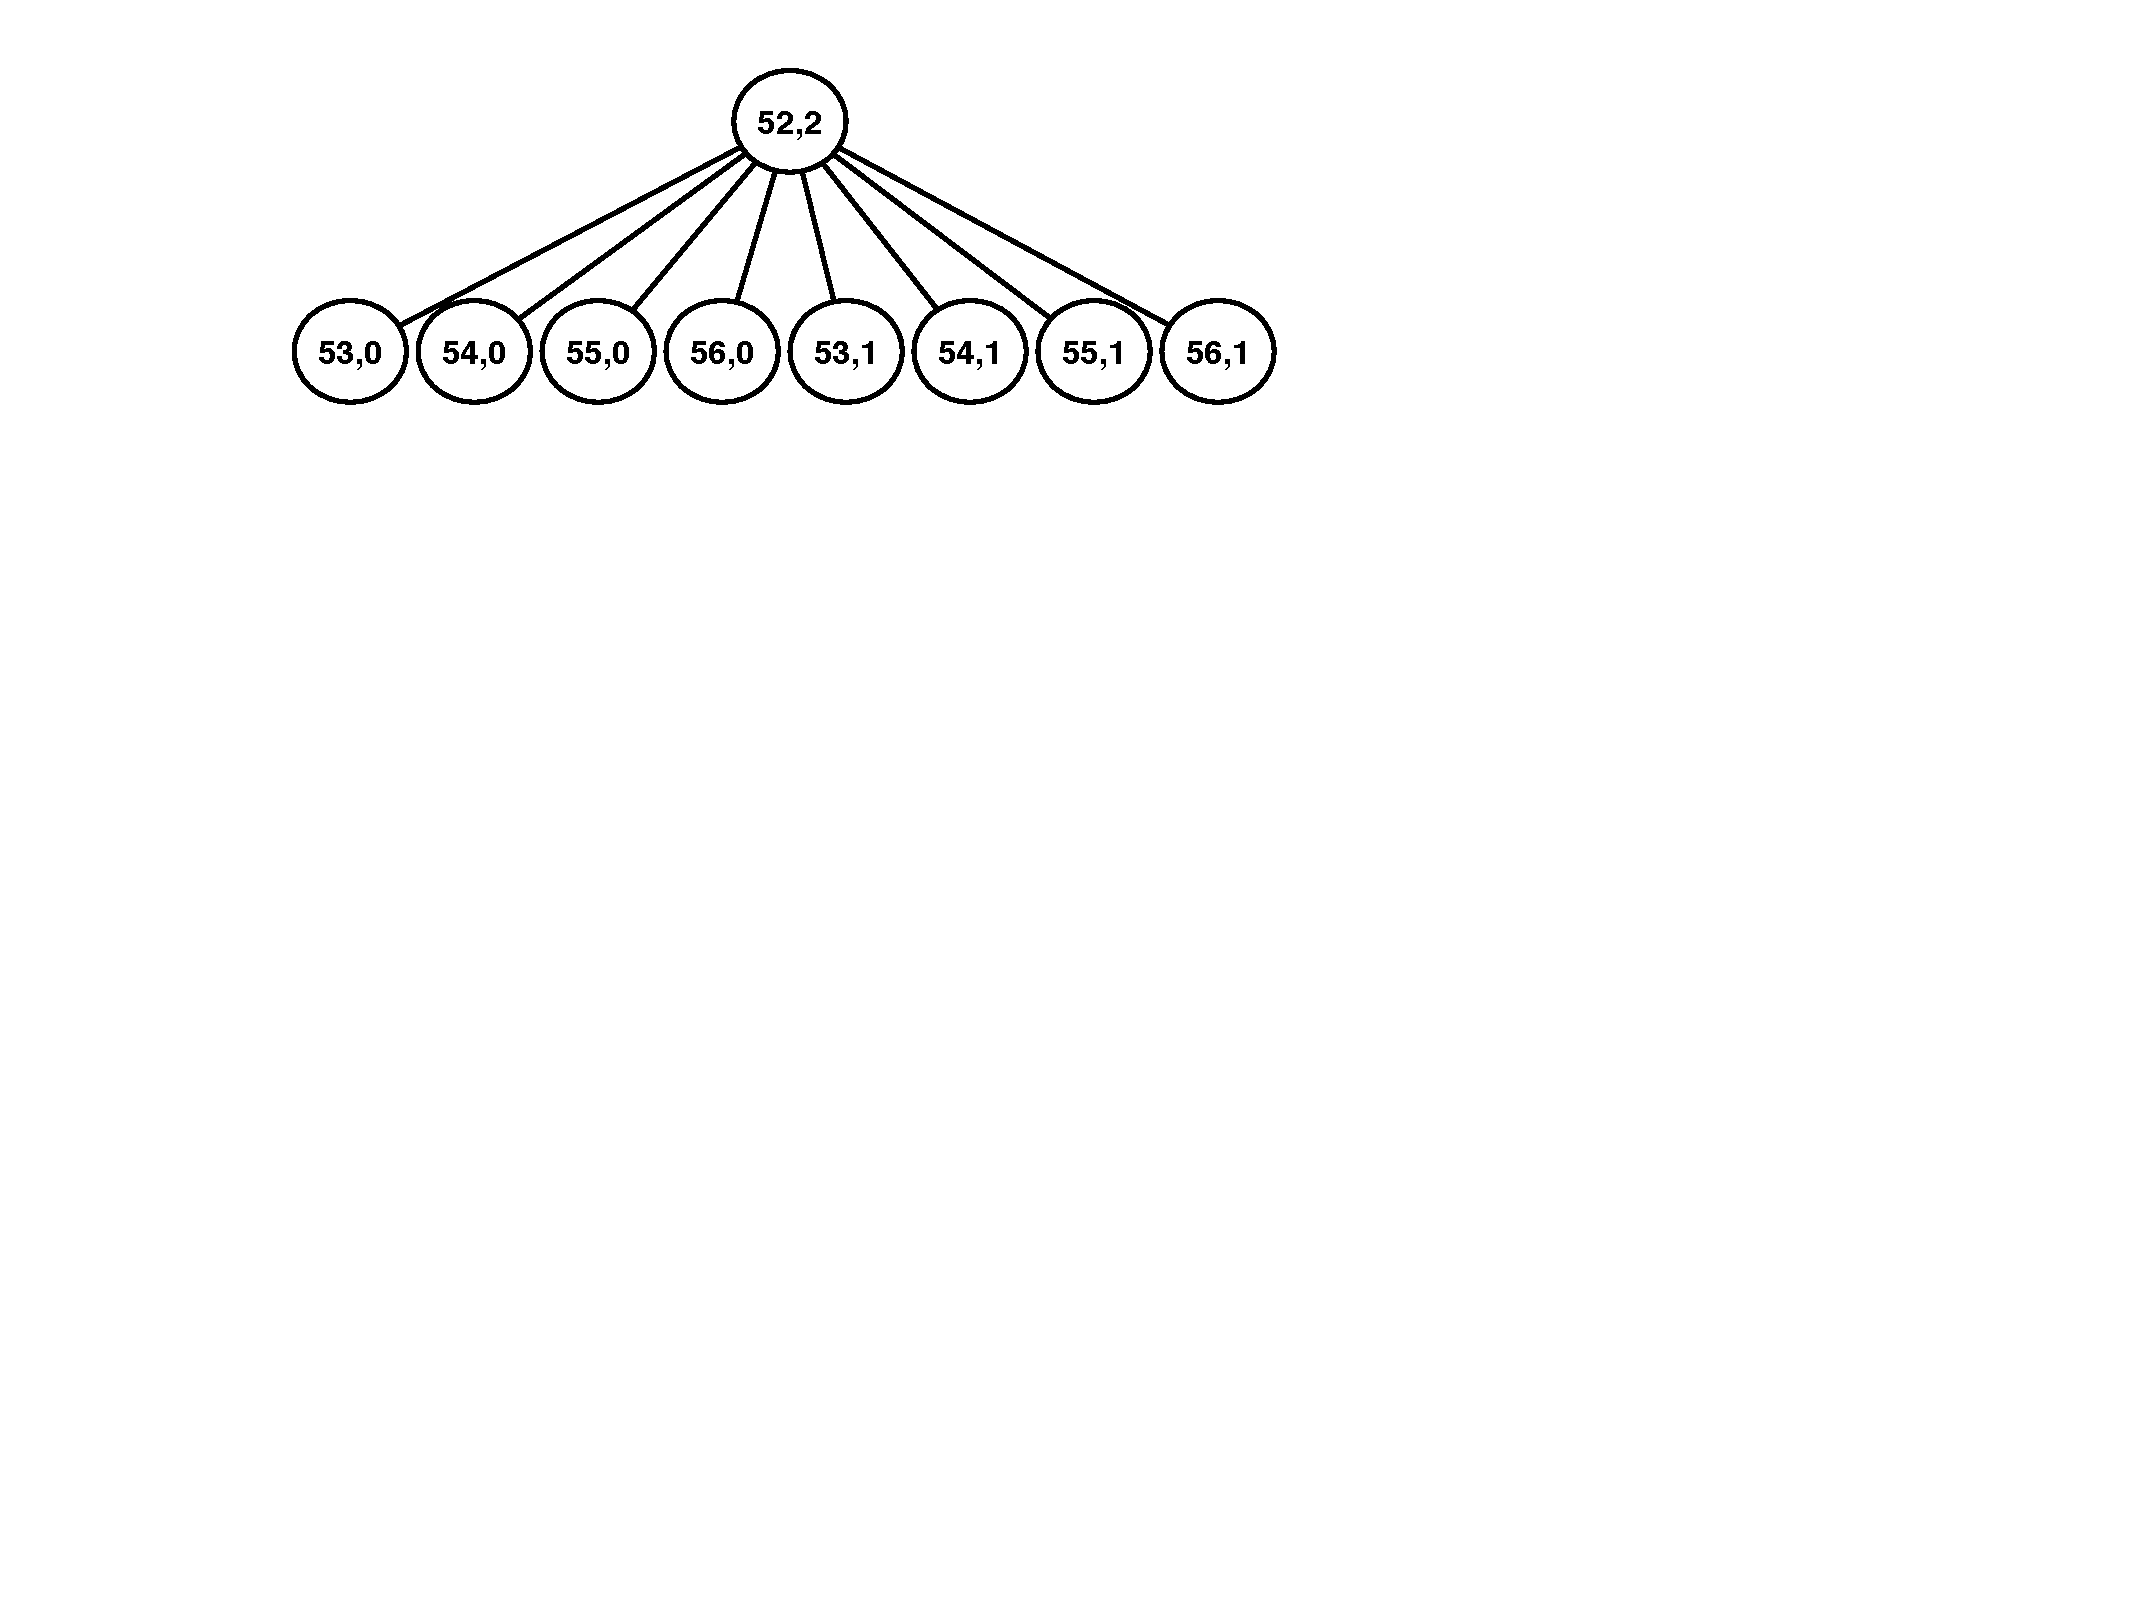
\includegraphics[width=60mm]{./Figures/bitTricks.pdf}
				\caption{An internal node with (simplified) label (52,2). The second number indicate that its $1/2$-approximation is  $2^2 = 4$. The children are given labels in  $\{53 \dots 56\}$ and an additional bit. }
				\label{fig:bitTricks}
			\end{figure}
			
			
 

%Suppose node $v \in T$  with traversal number $\dfsi(v)$ has $i$ children $c_1 \dots c_i$, and denote v's $1/2$-approx  $\lfloor v \rfloor $.
%Nodes $c_1 \dots c_{\lfloor v \rfloor }$  are given a label composed of their corresponding traversal number from $ \dfsi(v)+1 \dots \dfsi(v)+ \lfloor v \rfloor$ along with an each additional bit marked $0$.
%Each node in $c_{\lfloor v \rfloor+1} \dots c_i$ receives    numbers as given by the traversal to $c_1 \dots c_{\lfloor v \rfloor}$, with their additional bit  marked as $1$.

\subsubsection{A  $\log n + O(\log^*n)$ labeling scheme}\label{sec:log-star}
To further reduce the size of the label, the authors use a special and recursive clustering on the tree $T$. 
The nice clustering  technique (Section~\ref{tec:clustering}) is modified to suit the needs of the labeling scheme.
Recall that for every $ 1 \leq x \leq n$ and any tree $T$, there exist a (nice) cluster partition dividing $T$ to  at most $n / x$ clusters, each having $O(x)$ nodes.
\begin{definition}
A cluster $C(u,v)$ (Def.~\ref{dfn:cluster}) is a \emph{single child cluster} if 
\begin{inparaenum}[\itshape  I.\upshape)]
\item it is a leaf cluster; or
\item it  contains at most two nodes; or
\item $u \leadsto v$ contains at least 5 nodes, $v$ has no children in $C(u,v)$, and $u$ has only one, i.e., the node on the path to $v$.  
\end{inparaenum}
A nice cluster partition   (Definition~\ref{dfn:nice-cluster-partition})  is a \emph{single child cluster partition} if all its clusters are single child clusters.
\end{definition}

We complete an omitted   proof of  Lemma 7  in~\cite{Alstrup02}. 
\begin{lemma}\label{lemma:nice_decomp}
Let $T$ be a rooted tree with $n$ nodes. For every  $ 1 \leq x \leq n /7$ there exist a single child cluster partition of $T$ of at most $n/x$ clusters, each containing $O(x)$ nodes.
\end{lemma}

\begin{proof}
Let $\cs$ be a  nice cluster partition for $T$ with $\vert \cs \vert \leq n/7x$ and each cluster contains $O(x)$ nodes.
We decompose every  internal cluster $C(u,v) \in  \cs$ which is  not a single child cluster to at most  seven single child clusters as described below. 

Assume  that $u \leadsto v$ contains 5 or more nodes, and  that  $v$ has  children in  the cluster $C(u,v)$. Denote an arbitrary child of $u$ not on $u \leadsto v$ as $u'$.
 $C(u,v)$ is decomposed to  the clusters $C'(u,v)$ and $C'(u,u')$, where $C'(u,u')$ is a leaf cluster consisting of the  children of $u$ excluding the one in the path $u \leadsto v$, and $C'(u,v)$ contains the rest of the nodes.
We use a similar procedure on  a cluster $C(u,v)$ where $v$ has more than one child.
It follows that a cluster $C(u,v)$ is decomposed to  at most two leaf clusters and one internal cluster $C'(u,v)$ that contains the path $u \leadsto v$.
Hence, all three clusters are single child clusters.

If  $C(u,v)$ contains more than two nodes, and  $u \leadsto v$ contains less than five, we decompose the cluster  in the following manner (illustrated in Figure~\ref{fig:crazyeleven}).
An internal 2 node cluster $C(i,j)$ is created for every two adjacent nodes $i$ and $j$ on the path $u \leadsto v$.
In addition, a leaf cluster $C(a,b)$ is created  for every node $a$ on $u \leadsto v$  with at least one child not on the path.
Let $\mathcal{F}_d$ be the forest created by removing all edges on the path $u \leadsto v$ from the cluster $C(u,v)$.
Each cluster contains all the nodes in the tree rooted in $a$ from $\mathcal{F}_d$, and $b \neq a$, an arbitrary  node in $\mathcal{F}_d$.
To conclude, $C(u,v)$ is transformed to at most three single child internal clusters, and at most four leaf clusters.
\end{proof}

				\begin{figure} 
				\centering
				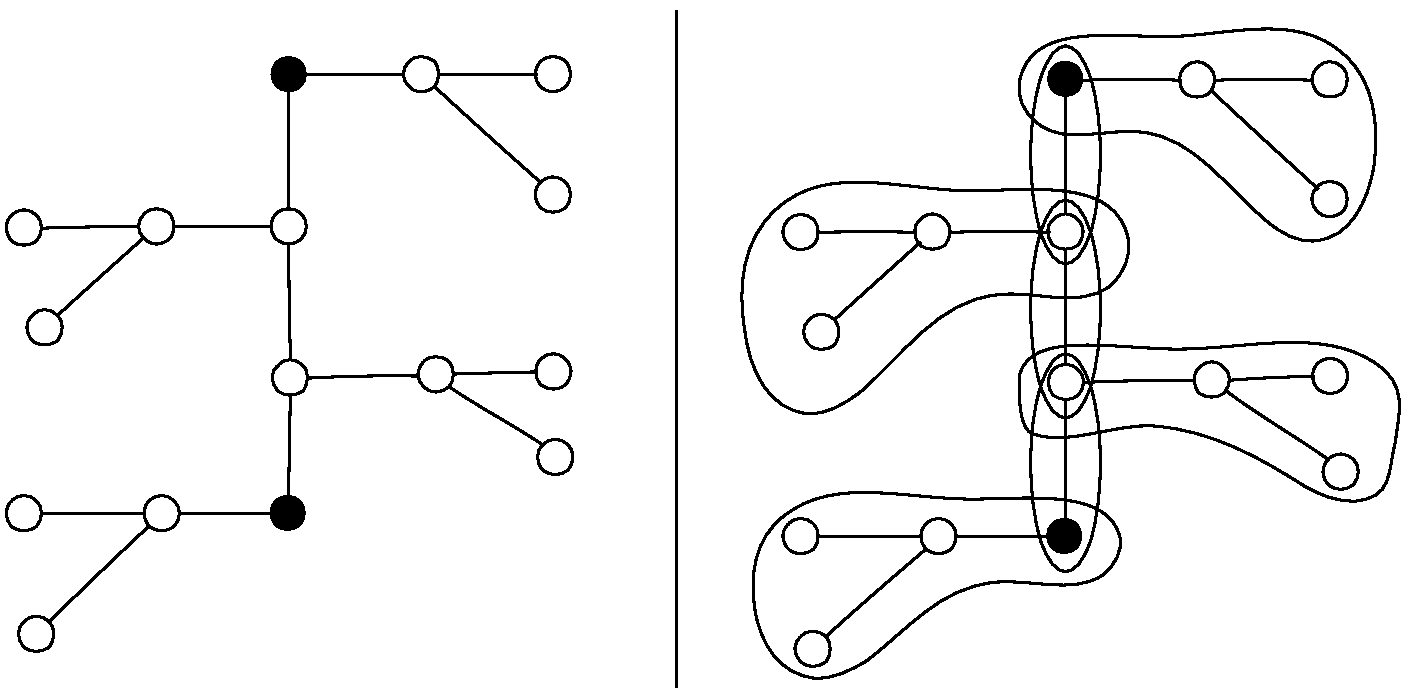
\includegraphics[width=80mm]{./Figures/7.pdf}
				\caption{Left: A nice cluster, Right: the cluster decomposed to 7 single child nice clusters. Black nodes are boundary nodes.}
				\label{fig:crazyeleven}
			\end{figure}
			
			

The cluster partitioning guaranteed in Lemma~\ref{lemma:nice_decomp} is used to  create a correlating \emph{macro tree}.
\begin{definition}\label{dfn:macro-tree}
A cluster partition $\cs$ has  a \emph{macro tree} $T_m$ defined as follows. 
The nodes $V(T_m)$ are the set of boundary nodes of  $\cs$.
The edges $E(T_m)$ are the set of pairs $(u,v)$, where $u,v$ belong to the same cluster $C(u,v)$. 
The root of $T_m$ is the root $r$ of the original tree $T$.
This is possible since $r$  is defined to be a boundary node of some cluster in $\cs$.
\end{definition}


			
			
\begin{theorem}\label{theo:adjacencytreesupper}\cite{Alstrup02}
There exist an \adjacency labeling scheme for $Trees(n)$ whose worst-case label size is at most $\log n + O(\log^* n)$.
\end{theorem}

\begin{notproof}[ sketch]
We begin by  labeling the macro tree $T_m$ (Def.~\ref{dfn:macro-tree}) of a single child cluster partition of $T$, using the  leaf favouring encoder $e_\beta$ (defined in  Lemma~\ref{lem:4loglogn}).
Every edge $(u,v) \in E(T_m)$ represents a \emph{micro tree}, a cluster  of at most $cx$ nodes, for some $c$, not including its boundary nodes.
In addition, $T_m$ has at most $n/x+1$ nodes.
We can use  $e_\beta$ to encode the leaves of $T_m$ using $\log(n/x)+O(1)$ bits, and the inner node of $T_m$ using $\log(n/x)+4\log\log(n/x)$. 
By choosing $x = \log^5 n$ both label sizes are bounded by $\log n + O(1)$.  
For the remainder of the proof, an edge $(u,v) \in E(T_m)$ where $\dfsi(u)<\dfsi(v)$ is labeled in $v$'s label,  $\la(v)$.

Consider the  nodes  in the internal cluster $C(a,b) \setminus \{a,b\}$.
These nodes maintain adjacency relation only between themselves and possibly the two boundary nodes $a$ and $b$.
By storing only a unique identifier of the edge they belong to in the macro tree, we can safely reject a query of two nodes from different clusters.
 Such a unique label is already given to every micro-tree labeled $\la(b)$  by $\dfsi(b)$, which is just the first $\log(n/x)$ bits of the label given by $e_\beta$. For illustration, see Figure~\ref{fig:Clustering}.
We stress that  the non-boundary nodes of the internal clusters are exempt from maintaining the additional $4\log\log(n/x)$ bits required by $d_\beta$ to determine \adjacency in $T_m$. 
We now mark the  boundary nodes, and their immediate (single) neighbours from each side by a finite number of types (such as root of an internal cluster, a child of a root of a cluster etc.).

				\begin{figure} 
				\centering
				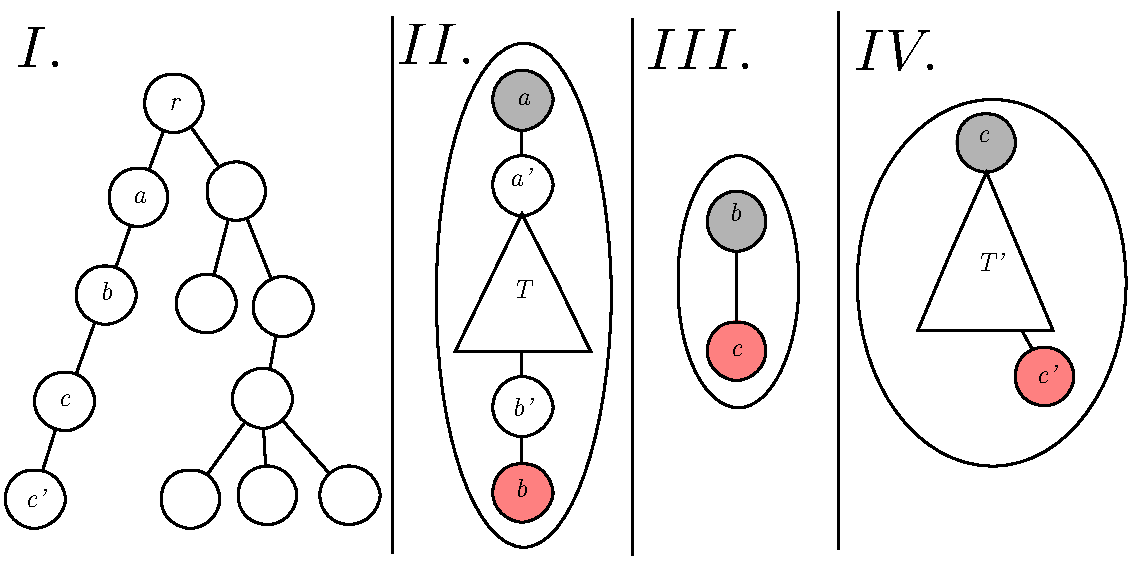
\includegraphics[width=90mm]{./Figures/MacroTreeNew.pdf}
				\caption{From left to right: \begin{inparaenum}[\itshape  I.\upshape)]
\item  A  macro tree $T_m$ with boundary nodes $a,b,c,c'$;
\item the internal cluster $C(a,b)$;
\item the internal cluster $C(b,c)$; and
\item the leaf cluster $C(c,c')$.  
\end{inparaenum} According to the labeling scheme the nodes in $T$ rooted by $a'$ store only the unique identifier of node $b$ in $T_m$, rather than the entire $\la(b)$ assigned to the node in $T_m$.  The last node in the $\dfsi$ traversal of $T$ is $b'$. }
				\label{fig:Clustering}
			\end{figure}
			
A full label for the tree is achieved by concatenating those labels with the \adjacency labels of  the micro trees, using the original   $\log x + 3\log \log x$  bits labeling scheme for trees of size $x$. This time  the boundary nodes  are the one exempt from  storing this information. The decoder can detect if  two nodes are in the same micro tree using the first part, and  check for \adjacency if the  two nodes  are in the same micro part, using the  second part of the labels. 

To summarize, there are now four types of nodes. Nodes in  leaf clusters, boundary nodes of the internal clusters, immediate neighbors of the boundary nodes, and nodes in micro trees of internal clusters.
All four now enjoy a labeling scheme of at most $\log n + 3 \log \log \log^5 n+ O(1)$.  

At this point the authors utilise the structure of the new micro trees and label those by applying the labeling scheme recursively.
The encoder  assigns $\la(u)$ to $u \in T$ as a concatenation of at most $i$ decreasing size macro trees that contain $u$.
The last element concatenated to $\la(u)$ marks that $u$ is  either be a boundary node in some level prior to $i$, or a full label of $u$ in the last micro tree.
Denote $f(n) = log^5(n)$ and $f^i(n)$ operating $f$ $i-1$ times recursively on $n$.
$e_\beta$ is applied $i-1$ times, and nodes in the (final) micro trees are labeled by the second encoder $e_\alpha$.
The  description of  the labeling scheme  yields  labels of size at most:
\begin{dmath}
	 \sum_{j=1}^{i} \left( \log{(f^{j-1}(n)/f^{j}(n))} + O(1) \right) + 3\log \log{(f^{i-1}(n)/f^{i}(n)}) +O(1)  = \log{n} + \log{f^i(n)} +  i \cdot O(1) + 3\log \log{(f^{i-1}(n)/f^{i}(n))}. 
\end{dmath}
Assigning $i= \log^* n$ we have that the maximum label size is $\log n + O(\log^* n)$ as guaranteed.
\end{notproof}


\subsection{Traversal and jumping}\label{traversaljumping} 			
			Caterpillars were shown to have a labeling scheme of $\log n+{O}(1)$ by \citeN{Gavoille06},  using a technique called ``traversal and jumping". In the remainder of this section we occasionally refer to the labels as the integers they represent.
			
A caterpillar tree $T$ rooted in $x_1$ consists of the  path  of \emph{internal nodes} $P = x_1 \dots x_{p}$ where each $x_i \in P$ has $l(i)$ \emph{leaf children} $L(i) = y_1^i \dots y_{l(i)}^i$.
The only two cases where two nodes are adjacent in a caterpillar is either when one is a leaf child of the other or if they are  adjacent internal nodes. 
We also note that  there exist a straightforward  non-unique \adjacency labeling scheme for this family.

Recall that  a $\dfsi$  traversal (Section~\ref{sec:efficient-encoding}) of a   caterpillar $T$  rooted in    $x_1$ visits nodes in $L(i)$ before  $x_{i+1}$ for all $1 \leq i \leq p $. As with the labeling scheme in Section~\ref{sec-adj-lb}, the leaves do not contain additional information other than a unique identifier. For every $1 \leq i \leq p $ and $1 \leq   j \leq l(i)$, we set $\la(y_j^i) = \la(x_i)+ j$.  In other words, the leaf children of $x_i$ are given labels  consecutively after $x_i$'s label, and a single bit is  prefixed to each label to determine the node's type.  

 We can construct a  $2 \log n$  \adjacency labeling scheme by assigning $\dfsi(v)$ to every node $v$, and concatenate    $l(i)$ to  every internal node.
 An internal node $u$ and a  leaf child $v$ are adjacent if and only if  $\dfsi(u) \leq \dfsi(v) \leq \dfsi(u)+l(i)$, and two internal   nodes $u$, and $v$ where $\dfsi(v)>\dfsi(u)$ are adjacent if and only if  $\dfsi(u)+l(u)+1= \Id(v)$.
 
Rather than storing  $l(i)$ in $x_i$, we  maintain a 2-approximation (Section~\ref{tec:approx}) of both $l_i$ and $l_{i+1}$ denoted 
$\ceil{l_i}_2$ and $\ceil{l_{i+1}}_2$, respectively in $x_i$. For $1 \leq i \leq p$ we compute  $$t_i := max\{ 2 \log{t_{i+1}}, \log(\ceil{l_i}_2 )\}+O(1),$$ where $t_{p} =  \log(\ceil{l_p}_2)$. An  internal node $x_i \in P$ is assigned a range of size $2^{t_i}$ in which the label of $x_i$ and the labels of $L(i)$ will reside.  
In order to store both $t_i$ and $t_{i+1}$ in the label of $x_i$, we first construct the suffix code (Section~\ref{tec:suffix}) $C(x_i)$, which is defined as:
$$C(x_i)= code_1(t_{i+1}) \circ code_0(t_i - \vert code_1(t_{i+1}) \vert ).$$
We  then choose the  label of $x_{i+1}$ to be   the  number in the range  
$\{\la(x_i)+2^{t_i} \dots \la(x_i)+2^{t_i} + 2^{t_{i+1}}\}$ that  contains $C(x_i)$ as a suffix.
 We find this particular number using Lemma~\ref{lemma:numberinside}. Due to the selection of $t_i$, it is guaranteed that there are at least $l(i)$ consecutive numbers in the range after that number.
To prove that the size of the label  is at most $\log n + O(1)$ the authors prove that for some constant $c'$:
 $\sum_{i=1}^p 2^{t_i} \leq  c' \cdot \sum_{i=1}^p l(i)$. 
 %For completeness the proof is given in Appendix~\ref{AppendixC}.
  Since $\sum_{i=1}^p l(i) < n$, it follows that the maximum label size used by any internal node is $\log n +O(1)$.  
 The largest label is assigned to the last leaf $\la(y_{l(p)}^p)$, and since the leaves are assigned numbers consecutively after their parents, the number of labels is at most doubled, requiring only one additional bit. For an illustration of the technique see Figure~\ref{fig:caterpillar}.


				\begin{figure} 
				\centering
				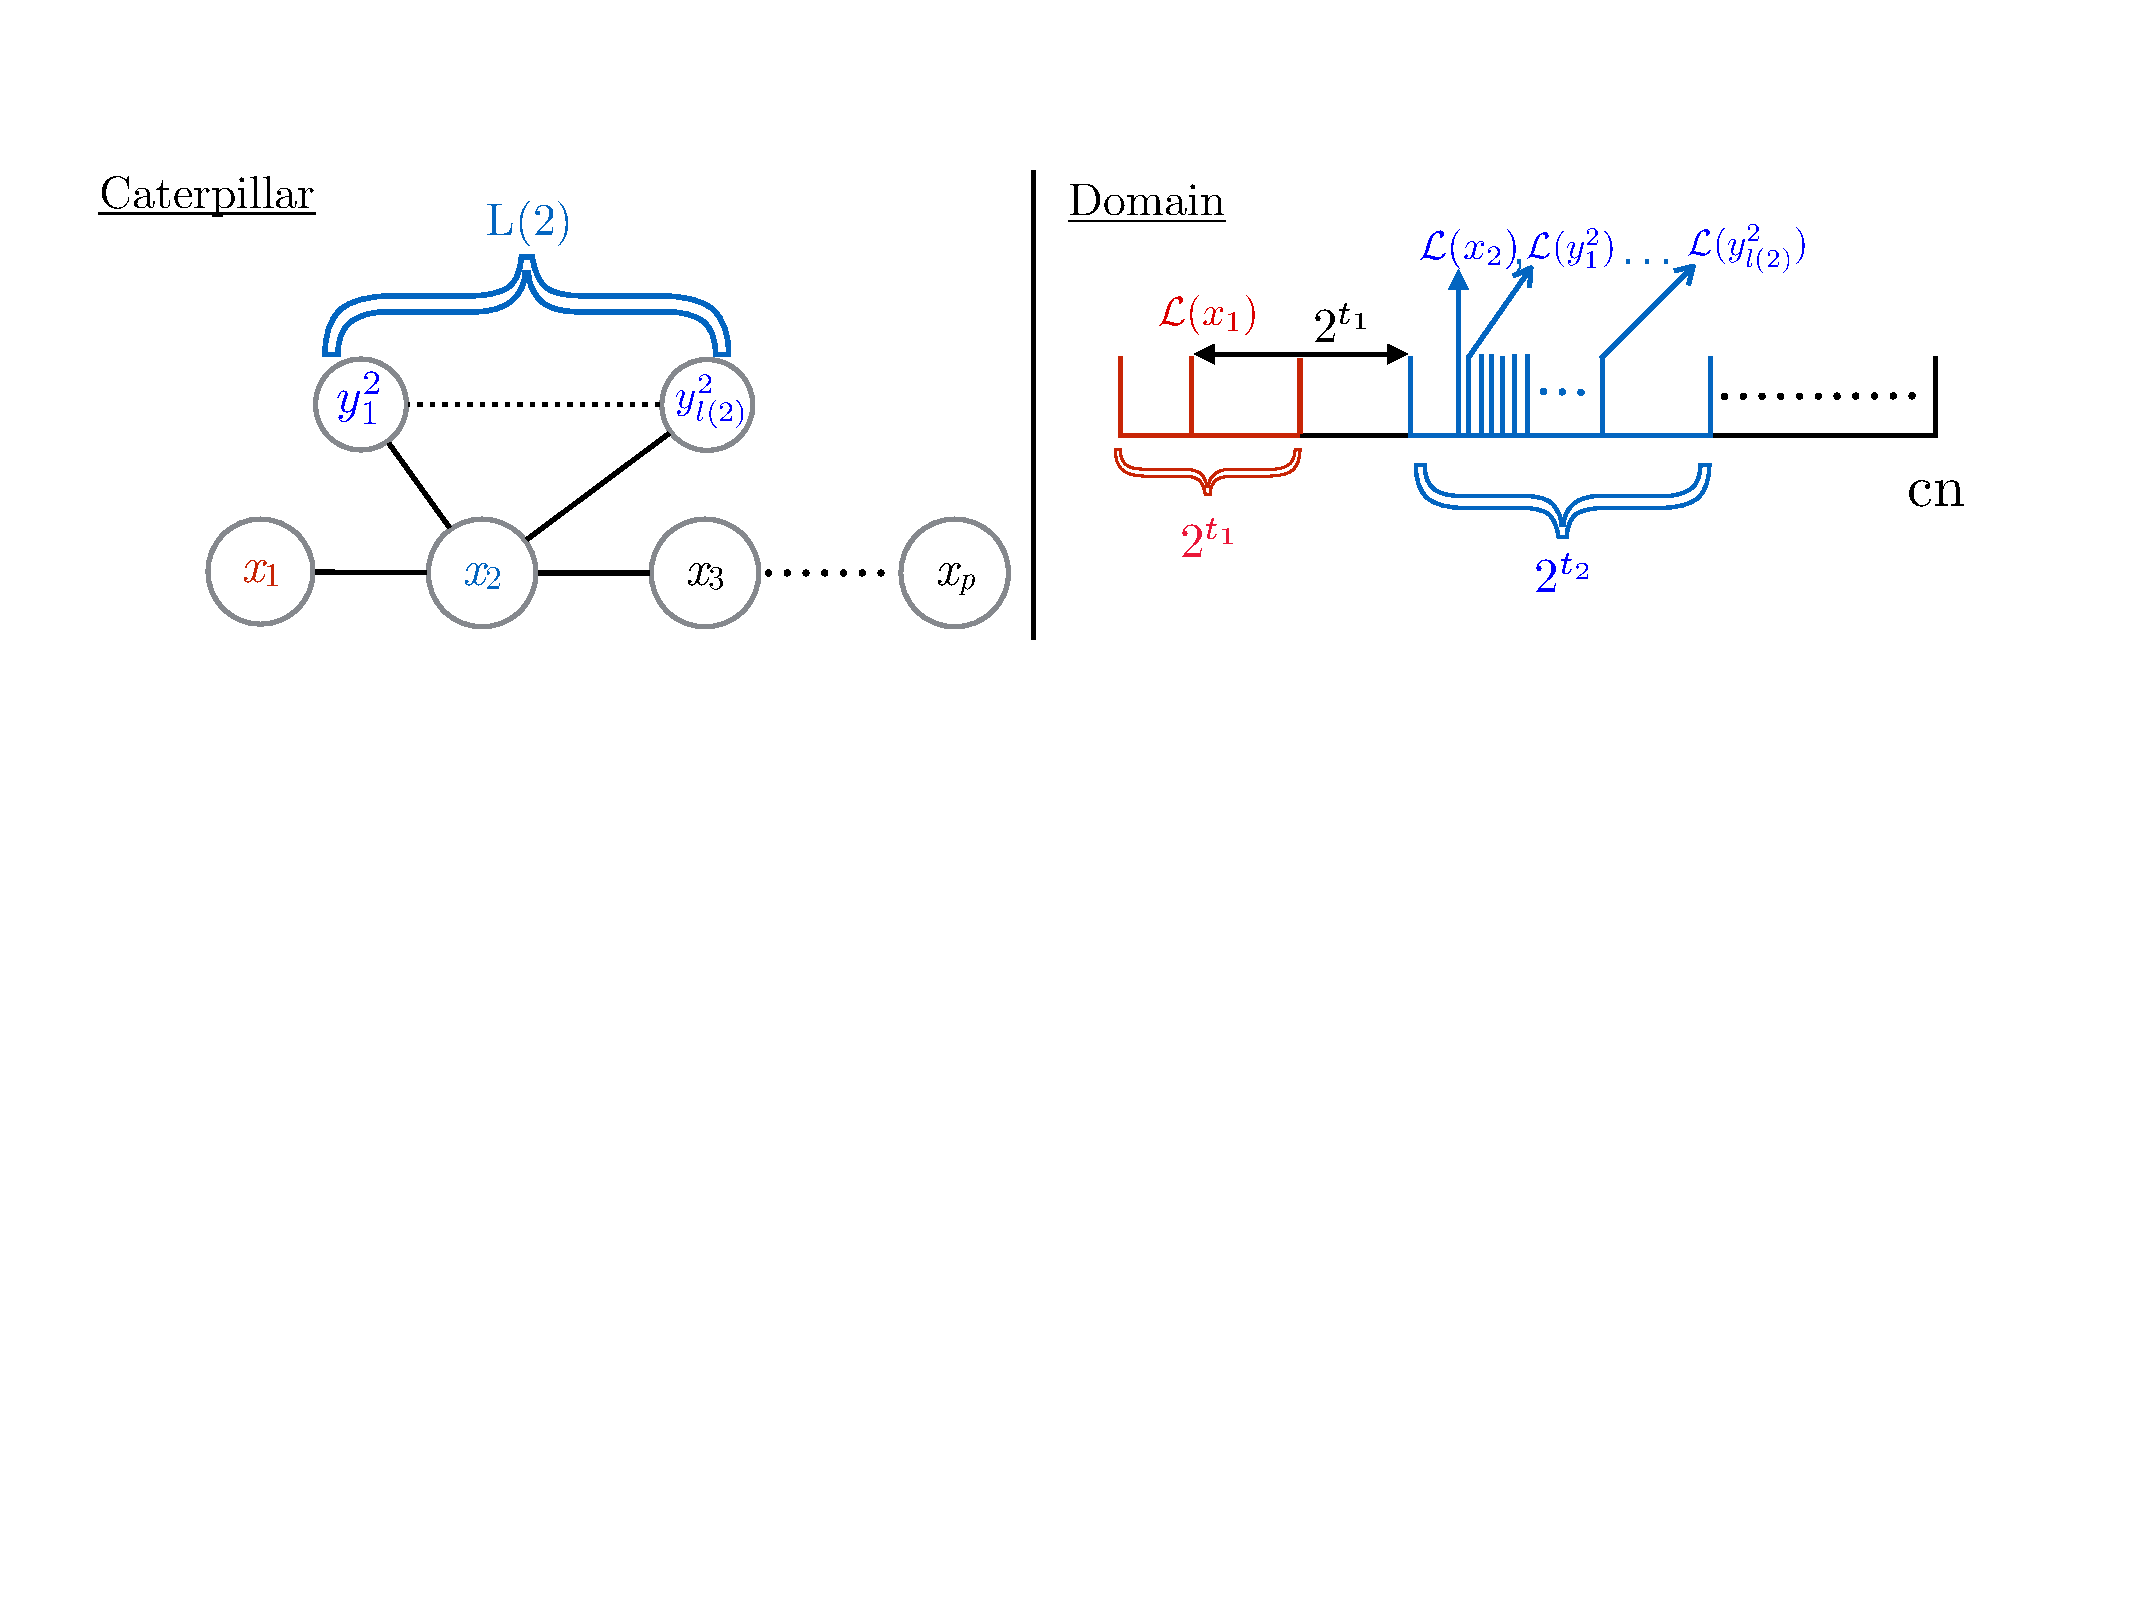
\includegraphics[width=120mm]{./Figures/Caterpillars.pdf}
				\caption{Label assignment of the inner nodes and leaves of the caterpillar depicted on the left using traversal and jumping. 
				The label  $\la(x_1)$ is chosen from $\{1 \dots 2^{t_1} \}$,  $\la(x_2)$ from $\{\la(x_1)+2^{t_1} \dots\la(x_1)+2^{t_1}+2^{t_2} \}$ and the  leaves $y_1^2 \dots y^2_{l(2)} \in  L_2$ are labeled s.t.  $\la(y_1^2) = \la(x_2)+1 \dots  \la(y^2_{l(2)}) = \la(x_2)+ l_2$.}
				\label{fig:caterpillar}
			\end{figure}


\paragraph{Optimal bounded degree}		
		Recently, \citeN{adjiashvili2014labeling} proved the existence of a labeling scheme for  $Trees(n, \Delta)$ with label size of  $\log n+O(\log \Delta)$.
		The labeling scheme is based  on an embedding technique of Bhatt, Chung, Leighton and Rosenberg~\shortcite{BCLR}.
		Bhatt et al.  showed the existence of an induced universal graph with   $O( \Delta \cdot  n)$  nodes that contains the family $Trees(\Delta,n)$. Although the construction was explicit, it is unknown how to produce efficient  decoder to match the possible encoding suggested by the construction.
		
		 \citeN{adjiashvili2014labeling} noticed that the simple construction in \cite{BCLR} (Lemma~3)  can produce a $\log n +O(\Delta)$ labeling schemes for the family, where the label is a concatenation of a node and edge identifiers.
		 More precisely, the label $\la(u)$  of node $u$ with parent $w$, has two parts: $u$'s unique number and the  local number of the edge $(u,w)$ in the universal graph.
		 The major problem is to determine at which point in the binary  string the first part  stops and the second part starts. To that end the authors used the label size as an additional input for the decoder.

\subsection{One-sided error \adjacency labeling scheme}\label{sec-adj-onesided}
		Consider the function \nonadjacency  for any graph $G= (V,E)$ that returns true if and only if  nodes $u,v \in V$   are \emph{not} adjacent in $G$.
		Suppose we  demand  our query to be precise only  when the nodes are in fact adjacent, and allow two non adjacent nodes to be declared adjacent.
		It is of course helpful to be able to predict and control how often such a ``false positive'' would occur.
		\cite{fraigniaud2009} demonstrate the usefulness  of one-sided error labeling scheme (Definition~\ref{dfn:one-sided}) for \adjacency in the following.	
			\begin{theorem}
			For any $1 \leq k $ there exist a one-sided error \nonadjacency labeling scheme  $\tuple{e,d}$  for $Trees(n)$ with guarantee $p = 1- \frac{1}{2^k}$ of size $2(k+1)$.
			Furthermore, $e$ is computed in $O(n)$, and $d$ is computed in $O(1)$
			\end{theorem}
			\begin{proof}
			For each node $v \in V$ in the tree $T=(V,E)$, $e$ assigns  $\la(v) = \tuple{\la_1(v),\la_2(v)}$  as follows.
			 The root $r$  is assigned $\tuple{\la_1( r ), \la_2( r )}$, where $\la_1( r )$, $\la_2( r )$ are chosen uniformly at random in  $ \{0 \dots 2^{k+1}-1 \}$. 
			A node $u$ with parent $v$ in the tree is assigned $\la_1(u) = \la_2( v )$ and $\la_2( u )$ chosen uniformly at random in  $ \{0 \dots 2^{k+1}-1 \}$. 
			 $e$ is clearly computed in $O(n)$ with $n+1$ calls to a random function, and may assign non-unique labels.
			 
			 The decoder $d$ will decode $ \tuple{\la_1( u ) , \la_2( u )},\tuple{\la_1( v ) , \la_2( v )}$  by evaluating  the predicate  $(\la_1( v ) =  \la_2(u))  \vee  (\la_1( u) =  \la_2(v)) $.	
			  If $u,v \in V$  are  adjacent, the predicate is trivially  satisfied.
			 If $u,v \in V$  are  non adjacent, $prob(\la_1( v ) =  \la_2(u)) = prob(\la_2( v) =  \la_1(u)) = \frac{1}{2^k+1}$.
			 Therefore, the predicate is satisfied with probability
			  $\frac{1}{2^{k+1}} + (1 - \frac{1}{2^{k+1}})\cdot \frac{1}{2^{k+1}} < \frac{2}{2^{k+1}} = \frac{1}{2^k}  $
			  , and thus $p = 1-\frac{1}{2^k}$.	
			  \end{proof}
			Notice that one bit is sufficient to avoid  false determination of two  adjacent nodes as  non adjacent.
			The latter theorem shows that for ``false positive''  guarantee of   $99.99\%$, as few as 30 bits are sufficient.
			Choosing  $k= \log n+O(1)$  ensures  a guarantee   $p = 1-\frac{1}{2^{O(1)} \sqrt{n}}$. In contrast, \citeN{fraigniaud2009} prove that any  one-sided error  \adjacency labeling scheme for $Trees(n)$  with guarantee $p$ requires labels of  size at least  $\log n + \log p - O(1)$. 

\section{\NCA}\label{section:NCA}
% !TEX root = ../Survey.tex
	We now discuss  labeling schemes for the function \NCA. 
	Two variants of labeling schemes that support  the  function appear in the literature, \NCAl and \NCAf explained hereafter.
Suppose a tree $T=(V,E)$ has a predefined label assignment of $\log n$ bits  from a preset name domain, and denote  the product of such an  assignment for a  node $v \in V$  as the \emph{node identifier} of  $v$, or simply $\Id(v)$.  We can extend all labeling schemes presented so far to support node identifiers  by modifying their encoder to concatenate the node identifier to each label. In the case of \NCA such an extension is not as straightforward since it should return, for two nodes in the tree, the node identifier of  a third node.  We treat both variants, and denote labeling schemes for \NCA specifically designed to support node identifiers as \NCAf, and those that do not as  \NCAl.

In Section~\ref{sec:Lit-NCA} we provide  a literature overview and describe connections to related problems. In Section~\ref{sec-NCA-FIXED} we survey a  connection between \NCAf and the functions \distance,  \seplevel~ and \centerf. The connection leads to a lower bound, for which an asymptotically identical upper bound is presented. We  dedicate  Section~\ref{section-NCA-designer}  to the  construction of a \NCAl labeling scheme, of the same asymptotic size.
We then show how to improve  this labeling scheme to achieve labels of size $O(\log n)$. Finally, we  discuss  an  extension  of labeling schemes that  provides  a natural bridge between the two variants.

\subsection{Literature review}\label{sec:Lit-NCA}
The problem of finding nearest (occasionally referred, least) common ancestors (NCAs) is non-trivial already in the non-distributed setting. 
Its importance is derived by its role as a subroutine of common algorithms for minimum spanning trees in a graph, finding maximum weighted matching in a graph, and bounded tree-width algorithms.
Aho, Hopcroft and Ullman~\shortcite{aho} were among the first to consider the problem of finding NCAs, and \citeN{hareltarjan} were the first to describe an algorithm that uses only linear time and space for pre-processing and can answer \NCA queries in constant time.
Their algorithm is distributed for complete binary trees, but uses a non-distributed, precomputed auxiliary data structure in order to generalise the results to arbitrary trees.
A more recent,  simpler, and  distributed algorithm was presented by \citeN{Alstrup02NCA} in the form of a \NCAl labeling scheme of size $10 \log n+O(1)$.  The labeling scheme was improved recently by~\citeN{Green14} to $3 \log n+O(1)$, along with a lower bound of $1.008n$, and a  non-constructive proof of a labeling scheme of size $2.772 \log n +O(1)$.
 
 \citeN{peleg2000informative} showed that  for \NCAf  labels of size $\Theta(log^2 n)$ are sufficient and required.
\citeN{blin2010fast} extend Alstrup et al.'s labeling scheme for labels of length bound by constant $k$.
 Experimental studies of  labeling schemes for the function are considered in~\cite{caminiti2009informative,Fischer09}.
~\citeN{Korman07K} studied \NCAf on a different model called  \emph{1-query}. In this model, the decoder has access to a \emph{query} function, that gets two labels and returns  a node identifier.  In this setting  \NCAf queries can be answered using labels of size  $O(\log n)$.
			
\paragraph{Connection to other problems}
The function \NCA  is tightly related to two problems.
First,  finding a nearest common ancestor labeling scheme is equivalent to the \emph{discrete range searching problem}~\cite{gabow}.
Second, for both \NCAf and \NCAl, the  labels produced can determine ancestry relation directly. 
Put formally, any labeling scheme $\tuple{e,d}$  supporting the  \NCA function computes a label assignment $e_T$  with following property:
For $u,v \in T$, we can construct a decoder that receives $\la(u),\la(v)$  determines ancestry.
The decoder may use the \NCA decoder $d$ and compare the result to $\la(u)$. If $u$ is a parent of $v$, the two are equivalent and our ancestry decoder may safely return \emph{True}.
As a result, any lower bounds that apply to ancestry labeling schemes apply to NCA schemes as well.
A last connection between  the function \NCA and routing is discussed in Section~\ref{section-NCA-designer}.

\subsection{\NCAf} \label{sec-NCA-FIXED}
In this section, we present lower and upper bounds for \NCAf.
	\subsubsection{\NCA, \seplevel, and their connection to \distance }
		\citeN{Peleg05} proved that  $\Omega(\log^2 n)$ bits are necessary for any \NCAf labeling scheme, as well as the functions \seplevel, and \centerf.
		Recall that the function \seplevel returns the length of the path  $r \leadsto w $ in $T$ where $r$ is the root and $w$ is $NCA_T(u,v)$.
			\begin{theorem} \cite{Peleg05}\label{NCAconnection}
			For  labeling schemes  on $Trees(n)$, we have the following claims:
			\mbox{}
			\begin{enumerate}
						\item Given an  $f(n)$ \distance labeling scheme, we can construct a $f(n)+\log n$-\seplevel labeling scheme.
			\item Given an  $f(n)$ \seplevel labeling scheme, we can construct a $f(n)+\log n$-\distance labeling scheme.
			\item Let g(n) denote the maximum size of an identifier of any node in $Trees(n)$. If an \NCAf labeling scheme has labels of size at most  $l(n) \cdot g(n)$ then  there exist a \seplevel labeling scheme of size  $ l(n) \cdot (g(n) + \log n).$ 
			\end{enumerate}
			\end{theorem}
			\begin{proof}
			To prove Claim 1, assume there exist a distance labeling scheme  $\tuple{e_{dist},d_{dist}}$. 
			The encoder  $e_{dist}$ computes a label assignment  for a tree  $T$ rooted in $r$ with nodes $u$, $v$ and $w$ such that  $w= \NCA(u,v)$.
			We transform the encoder $e_{dist}$ by concatenating a prefix  $\depth(v)$
			\footnote{ Section~\ref{definitions-of-trees}): A node $v$ in a tree $T=(V,E)$ rooted in $r$ has  $\depth(v)$  edges on the path $r \leadsto v$.}  to the label $\la(v)$ assigned by $e_{dist}$ to every $v \in V$, using additional  $\log n$ extra bits.
			The decoder can now compute \seplevel$(u,v)$, by   observing that 
			$\distance(u,v) = \distance(u,\NCA(u,v))+\distance(v,\NCA(u,v)) \text{, and } \depth(u)=\depth(\NCA(u,v))+\distance(u,\NCA(u,v))$
			 (the same formula holds by replacing $u$ with $v$).
			 It follows that  $$\depth(\NCA(u,v)) =  \frac{\depth(u)+\depth(v)-dist(u,v)}{2} = \seplevel(u,v).$$
			 We prove Claim 2  using the same transformation, i.e. adding $\depth(v)$	 to all labels produced by the encoder of any \seplevel labeling scheme.  
			 We prove Claim 3  by the same transformation, with the exception that  the new encoder adds $\depth(v)$ to the node identifier, adding exactly $\log n$ for  each of the node identifiers.
			\end{proof}
			
			\distance labeling scheme has a lower bound of $\Omega(\log^2 n)$ on the size of the label~\cite{gavoillea2004distance}.
			Assume that there exist a labeling scheme for \NCAf  of size $\phi(n) = o(\log^2(n))$. Since $g(n) = \log n$, it implies that $l(n) = o(\log n)$.
			By Claim 3, there also  exist a corresponding labeling scheme for \seplevel of size $o(\log^2 n)$.
			That labeling scheme, by  Claim 2, leads to a distance labeling scheme for distance of size $o(\log^2 n)$, in contrast with the lower bound mentioned~\cite{gavoillea2004distance}.
			
			\begin{corollary}
			Any labeling scheme supporting \NCAf for $Trees(n)$ must use labels of size $\Omega(\log^2(n))$.
			\end{corollary}
			 
\subsubsection{Upper bound for \NCAf}
It remains to prove that  there exist an \NCAf  matching (asymptotically) the lower bound.		 
For brevity, we repeat the definitions related to heavy-light decomposition (Section~\ref{tec:heavylight}):

$\hchild(v)$ is the (unique) heavy child of $v$,
$\lchildren(v)$ is the set of light children of $v$,
$\lsize(v)$ is the weight of $v$ not including the tree rooted in its heavy child,
$\lpath(v)$ is the list of all light nodes in  $r \leadsto v$,
$\ldepth(v) = \vert \lpath(v) \vert$,
$\hpath(v)$ is the set  of nodes on the same heavy path as $v$.


	\begin{theorem}\label{NCA-fixed-upper} \cite{Peleg05}
	There exist an \NCAf labeling scheme with labels of size at most $O(\log^2 n)$.
	\end{theorem}

	\begin{proof}
	Let  $T$  be a tree rooted in  $r$, where every node  $v \in V$ with light depth  $\ldepth(v)$ has   a unique  predefined identifier, $\Id(v)$.
%	 As proved in Section~\ref{tec:heavylight},  there are $1 \leq \ldepth(v) \leq \log n$ light nodes on  path between the root and any node  $v$ in $T$. 
 The label of node $v \in T$ is  defined as a concatenation of two parts, namely, $\mathcal{C}_a(v)$ and $\mathcal{C}_b(v)$ defined below.
	 
	 $\mathcal{C}_a(v)$   contains $\Id(v)$, and  an ancestry label as defined in Section~\ref{section:NaiveAncestry}, using at most $2 \log n $ bits, and in total at most $3 \log n $ bits.
	  $\mathcal{C}_b(v)$  contains a  concatenation (Section~\ref{section:Misc-Tools}) of triplets  of the form $\tuple{\Id(l_i),\Id(n_i),d_i}$, for $ 1 \leq i \leq  ldepth(v)$, where 
	 $l_i$  is the $i$'th light node in $\lpath(v)$, $d_i$ is the depth of $l_i$,  and $n_i$ is the node adjacent to $l_i$ on  $ r \leadsto l_i$.
	 Each triplet requires at most $3 \log n$ bits, and thus  $\mathcal{C}_b$ contains at most $3\log^2 n$ bits.
	 In conclusion, for every node $v \in T$,  $\vert \la(v) \vert = \vert \mathcal{C}_b(v) \vert  + \vert \mathcal{C}_a(v) \vert \leq 3(\log^2 n+ \log n)$.
	 
	We describe the operation on two nodes $u,v \in T$ with NCA $w$.
	The decoder  uses $\mathcal{C}_a$  to determine if one is an ancestor of the other, and if so returns its node identifier.
	At this point we can safely claim that  the path $u \leadsto v$ traverses exactly two  of $w$'s edges, where at least one of those  must be a light edge (see Figure~\ref{fig:NCAPeleg} for a demonstration).
	Thus, the decoder computes the common prefix of $\mathcal{C}_b(u)$ and $\mathcal{C}_b(v)$, and determines the first  $k$ for which the $k$'th triplet in $\mathcal{C}_b(u)$  is not equal to the $k$'th triplet in $\mathcal{C}_b(v)$.
	Since each triplet contains the depth of the light node it represents, we can deduce which of them is closer to $w$, and if the depth is equal we choose one arbitrarily.
	We  return the parent of the light node, stored in the selected triplet. 
	\end{proof}
	
					\begin{figure}[!ht] 
				\centering
				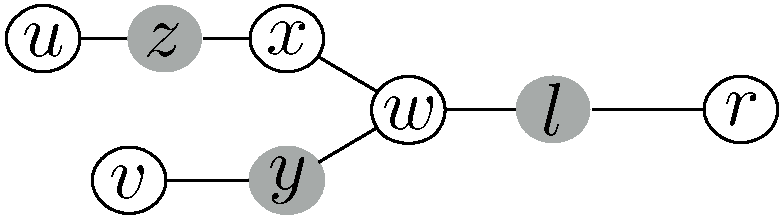
\includegraphics[width=60mm]{./Figures/NCApeleg.pdf}
				\caption{The nearest common ancestor w=\NCA(u,v) in a root rooted in r. The node  l is the last light node in common in the paths $r \leadsto u$ and $r \leadsto v$, and  $y$ and $z$ are the first light nodes immediately after $l$ on those paths, where $depth(z)>depth(y)$. Straight lines represent edges, dashed lines are paths, and grey nodes are light nodes. }
				\label{fig:NCAPeleg}
			\end{figure}
			
\subsection{\NCAl}\label{section-NCA-designer}
		We prove that there exist a \NCAl  labeling scheme of size  $O(\log n)$ in two steps.
		First, we present a simple (inefficient) labeling scheme with $O(\log^2 n)$  and then we prove that by a slight improvement, the label size decreases to $O(\log n)$. 
		 The first labeling scheme is by itself a modified version of the one presented in Theorem~\ref{NCA-fixed-upper}.
		Rather than storing the light path for every node along with the node above it, we store the light path along with the distance of the heavy paths  between each two consecutive light nodes. 
		\begin{theorem}\label{thm:nca-designer-long}
		There exist a \NCAl labeling scheme $\tuple{e,d}$ with label size bounded by $O (\log^2 n)$.
		\end{theorem}
		\begin{proof}
		Let $T=(V,E)$ be a tree rooted in $r$. For convenience,  $r$ is a heavy node with the  label $0$.
		We first compute a heavy-light decomposition of $T$ (Section~\ref{tec:heavylight}).

		The  new label   comprises the concatenation of the tuples  $\tuple{h_i,l_i}$, where $l_i$ is the index of  $i$'th light node  in $\lpath(v)$, and $h_i$ is the (possibly null) length of the heavy path $\hpath(l_i)$,  from $l_{i-1}$ to $l_i$ or to $v$ when $i=\ldepth(v)$.
		 See Figure~\ref{fig:NCAESBEN} for an illustration.
		 
		Since $1 \leq h_i, l_i \leq n$, each tuple requires at most  $2 \log n$ bits.
		Since $\vert \lpath(v) \vert \leq \log n$ (Section~\ref{tec:heavylight}), the total label size is bounded by $2\log^2 n$.
		To complete the proof we show how to compute the label of the NCA of two nodes $u$ and $v$ with labels $\la(u)= h_1^u,l_1^u \dots h_k^u,l_k^u$ and $\la(v) =  h_1^v,l_1^v \dots h_{k'}^v,l_{k'}^v $ respectively.
		 Without loss of generality assume that $k \leq k'$.
		We find the first $i$ for which $h_i^u,l_i^u \neq  h_i^v,l_i^v$.
		If there is no such $i$, then $u$ is the ancestor of $v$ and we return its label.
		 If $h_i^u = h_i^v$    we return the label $h_1^u,l_1^u \dots h_i^u$.
		 Otherwise, we return $h_1^u,l_1^u \dots  min\{h_i^u,h_i^v\}$.
		
		 \end{proof}	
		 
		 Note that this labeling scheme can return the depth of the NCA, in other words the \seplevel.
		 By Theorem~\ref{NCAconnection}, any   labeling scheme supporting \seplevel must have labels of size $\Omega(\log^2 n)$.
	 Moreover, using the formulas from Theorem~\ref{NCAconnection}  we observe that the function  \distance may also be computed using these labels.
		The first labeling scheme for the function \distance~\cite{Peleg00} uses separator decomposition.
		The label created in this labeling scheme  can not be used to determine the  functions \NCA, \adjacency and \ancestry.
		 In contrast, our  labeling scheme  stores enough information on the topology of the tree to determine all(!) the functions surveyed on trees.
		 
		The  labeling scheme presented is based on the ability  to choose a node's name. The one presented next utilises the ability further, and reduces the bound on the label size from $O(\log^2 n)$  to $O (\log n)$.
		\subsubsection{\NCAl with $O(\log n)$ bits}
		The maximum label size in Theorem~\ref{thm:nca-designer-long} is the longest description  of a sequence of at most $\log n$ tuples of the form $\tuple{h_i,l_i}$.
		 We do not  consider  assigning short labels to nodes with big size, nor do we account for the total length possible for the heavy paths.
		 However, even with those improvements, we will still be able to determine \seplevel, which implies a label of size $\Omega(\log^2 n)$ as mentioned.
		 
		 The key observation is that the function \NCA can be  determined even without knowing the exact length of the heavy paths.
		 We only require that each label of the nodes on a heavy path  $h_1 \dots h_k$ has a total order on that path, i.e., given two labels, determine which of them is first on the path.
		 Alstrup, Gavoille, Kaplan and Rauhe~\shortcite{Alstrup02NCA}  use those two  observations  as well as   Lemma~\ref{lemma:Gilbert}  to construct  a $O(\log n)$  \NCAl  labeling scheme presented below.

		\begin{theorem}\cite{Alstrup02NCA}\label{thm:nca-short}
		There exist a \NCAl labeling scheme  of  size  $O (\log n)$.
		\end{theorem}
		
		\begin{notproof}[Sketch]
		Consider a node $v$ where $parent(v)= u$ in a tree $T$ rooted in $r$ with $\ldepth(v) =k$ and  $\lpath= \{ lp_1 \dots lp_k \}$.
		The label  comprises the concatenation of the tuples  $\tuple{h'_i,l'_i}$.
		We first construct the labels given by  Theorem~\ref{thm:nca-designer-long} as auxiliary labels where   $\tuple{h_i,l_i}$  defined as in Theorem~\ref{thm:nca-designer-long}.
		
		To compute each $l'_i$, we use Lemma~\ref{lemma:Gilbert} with   $\size(lp_i)$ and the $\lsize$ of each of its  \emph{siblings}  in $T$.
		The lemma provides $l'_i$ a  label appropriate to $\size(lp_i)$, and more precisely:    
		$$\vert l'_i \vert  \leq  \log \size(v) -  \log \lsize(p(lp_i)) +1,$$
		where $p(lp_i)$ is the parent of $lp_i$.
		
		To compute each $h'_i$ we use  Lemma~\ref{lemma:Gilbert} with  the size of all nodes on the heavy path rooted in $lp_i$, $\hpath(v)$, ordered by their depth.
		That is, since we want to have labels as small as possible the closer we are to $lp_i$.
		The lemma provides $h'_i$ a  label appropriate to the light size of the $h_i$'th node on  $\hpath(v)$. More precisely:    
		$$\vert h'_i \vert \leq \log\size(lp_{i}) - \log\lsize(v) +1.$$
		
		In contrast to the previous labeling scheme, both $l'_i$ and $h'_i$ have variable size. In order to distinguish the different parts in $\la(v) = h'_1,l'_1, \dots h'_k,l'_k$ we use a separating string (Section~\ref{section:Misc-Tools}), which doubles the size of the label.
		By induction,  it can be shown that $\vert h'_1 \vert, \vert l'_1 \vert, \dots  \vert h'_k \vert ,\vert l'_k \vert  \leq \log n +4k +2$. The proof is similar to that of Lemma~\ref{lemma:tikun}.
		
		The decoder is computed similarly to the one defined in Theorem~\ref{thm:nca-designer-long} with the exception that in the last case we use  $\min_{\lex}\{h_i,h_i'\}$ instead of $\min{\{h_i,h_i'\}}$.
		
		For proof of the induction, and the correctness  of the decoder, see~\cite{Esben13}.
		\end{notproof}


					\begin{figure}[!ht] 
				\centering
				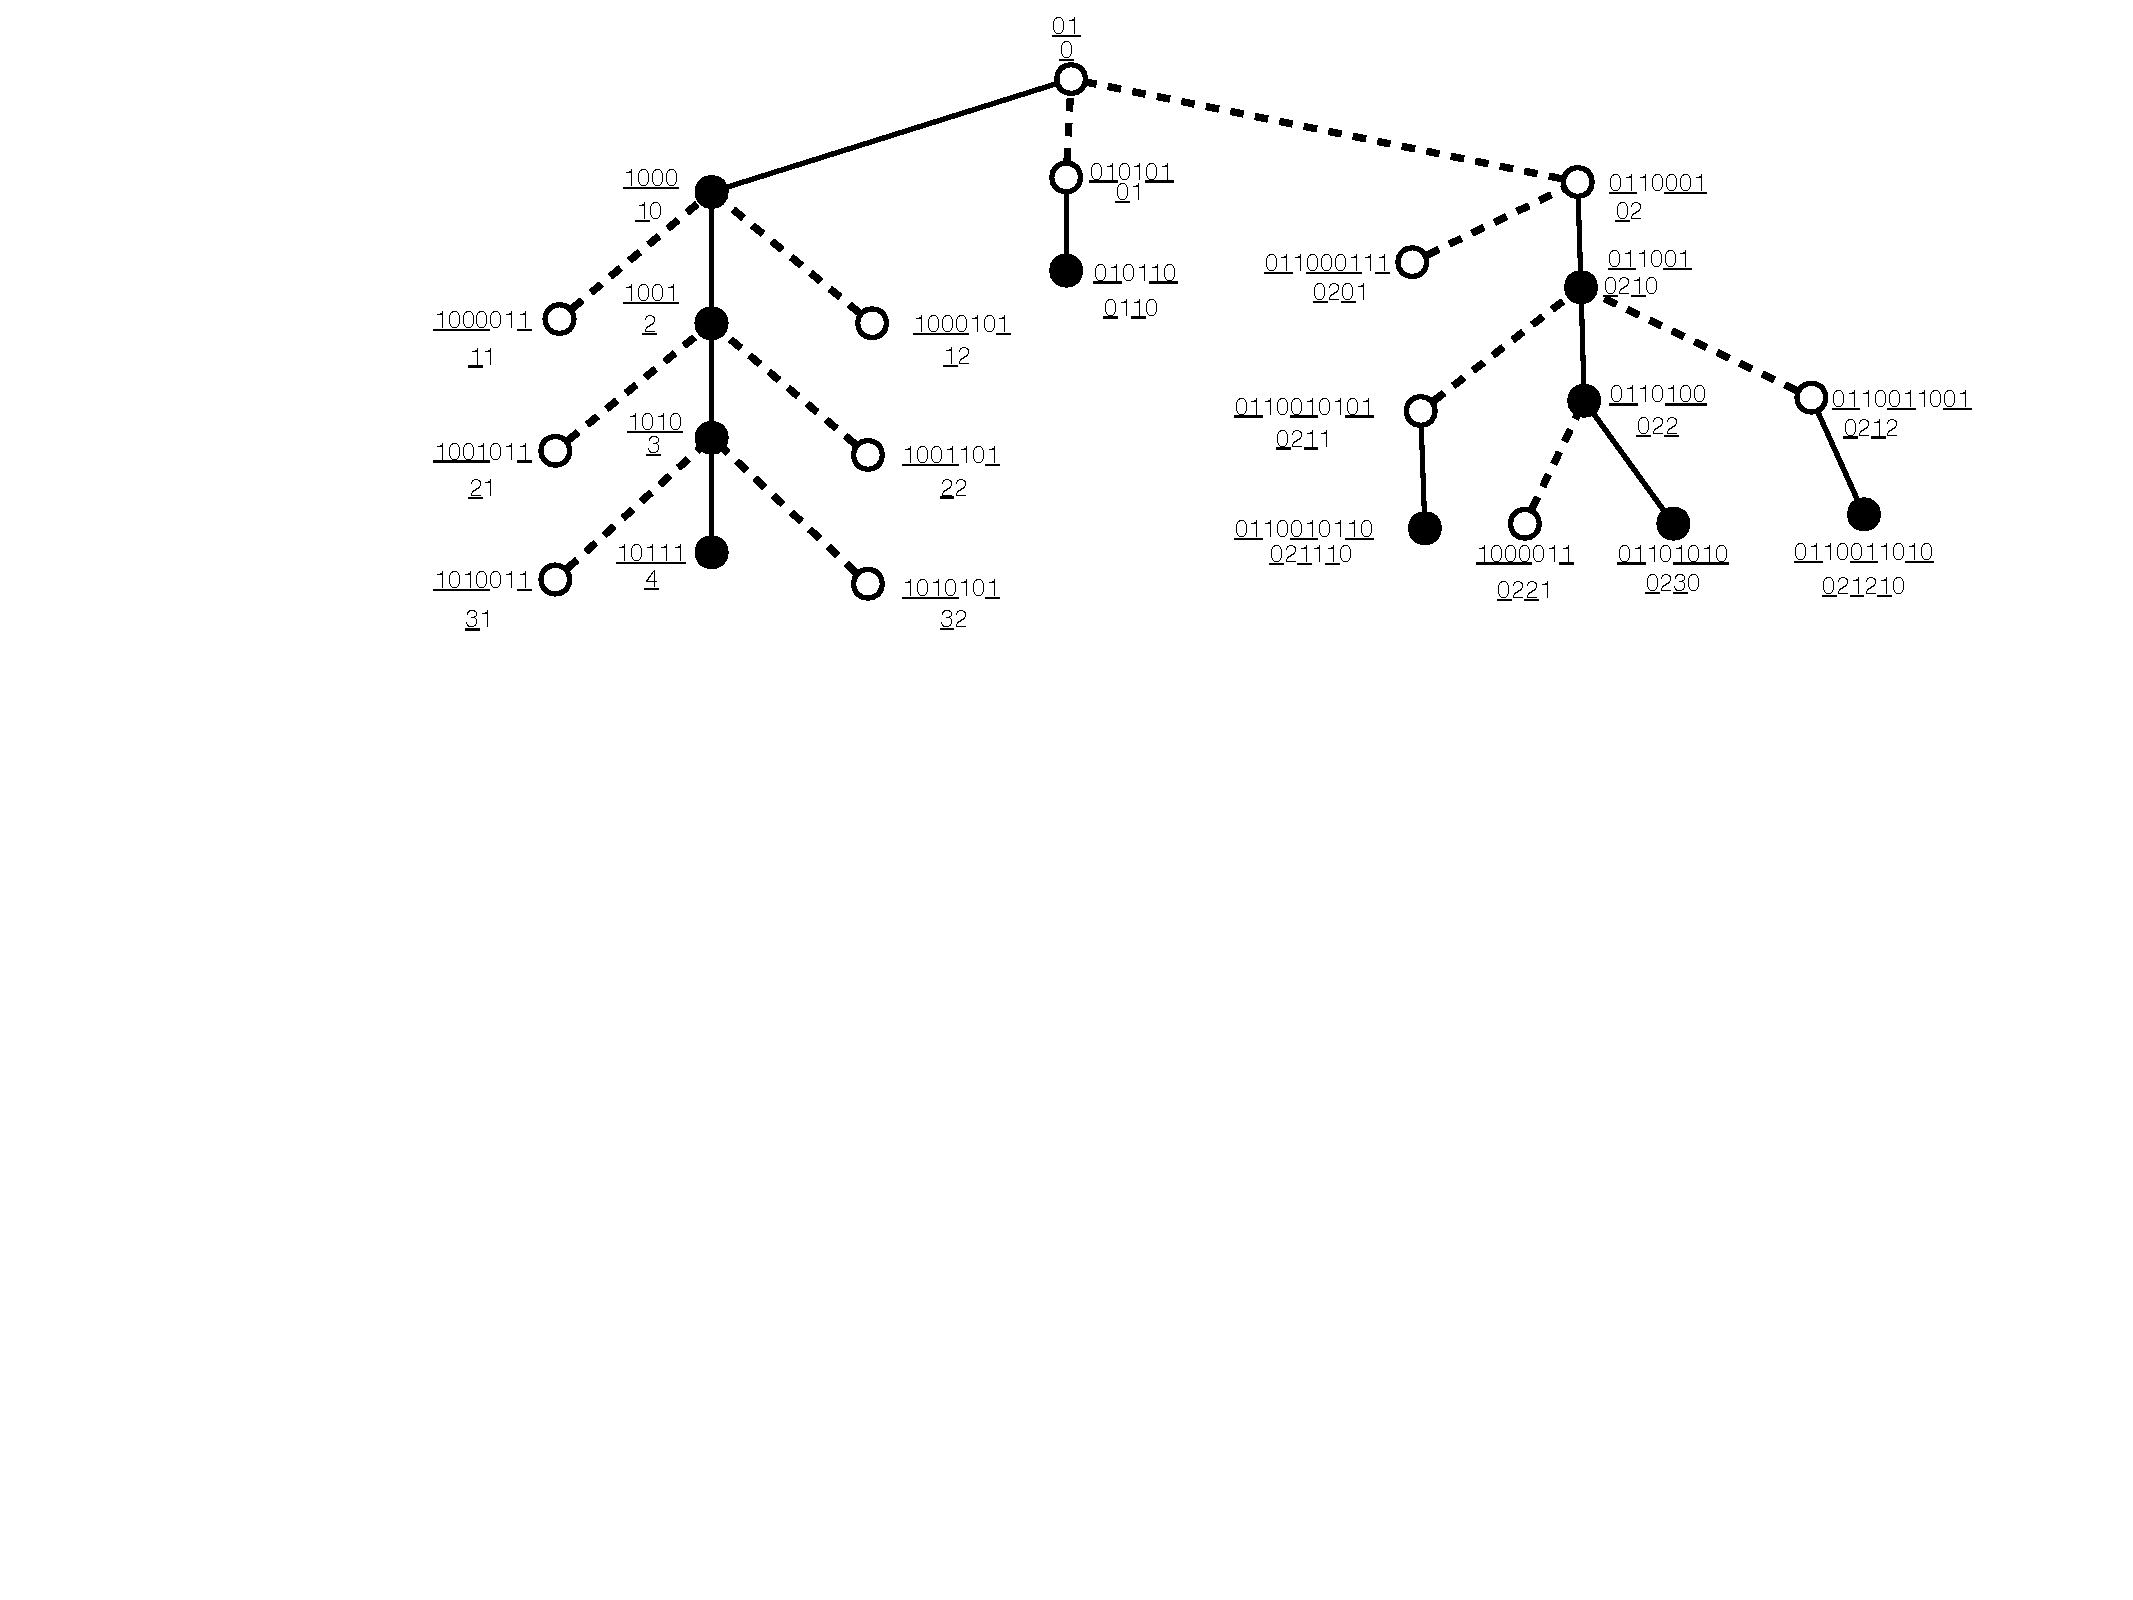
\includegraphics[width=120mm]{./Figures/Esbenscrazy.pdf}
				\caption{A tree with heavy (black) and light (white) nodes marked in the labeling scheme from Theorem~\ref{thm:nca-short} in binary on top and Theorem~\ref{NCA-fixed-upper} in decimal at the bottom. Both labels have their heavy sub-labels underlined.}
				\label{fig:NCAESBEN}
			\end{figure}
						
The labels constructed in Theorem~\ref{thm:nca-short}  can determine the first edge on the shortest path between the nodes queried. Therefore, using a slightly different decoder, we can construct a \routing labeling scheme (Section~\ref{section:Routing}).

The label size achieved in this method is at most $10 \log n$.
 \citeN{Green14} recently achieved an improved labeling scheme of size $3 \log n$ by replacing  Lemma~\ref{lemma:Gilbert} with a more compact  total order which allows for empty strings.

\paragraph{Labeling schemes with a query}
	  \citeN{Korman07K} extend  the definition of labeling scheme such that alongside the encoder and decoder, they define a \emph{query} function.
	Formally, given the labels $\la(u)$ and  $\la(v)$  of $u,v  \in  V $  outputs $Q(\la(u), \la(v))$ which is a node $ c \in V$.
	The decoder is free to use $c$ to compute the query.
	In this context, the authors proved that both  \NCAl and  \NCAf have a similar label size of  $O(\log n)$.
	The authors achieve similar label sizes for the functions \distance, \routing and \flow.
		
 

\section{\routing}\label{section:Routing}
% !TEX root = ../Survey.tex
We first describe general \routing schemes and two models for labeling schemes of \routing called \textit{designer port  model} and 
\textit{fixed port model}.
In Section~\ref{routing:literature} we  provide a literature review.
In Section~\ref{sec:ThorupZwick} we describe in detail the current best upper bound for routing in the designer port model due to \citeN{Thorup01}. We provide a corrected proof for this result.
In Section~\ref{sec:ThorupZwickFixedPort}  we  present a proof omitted in \citeN{Thorup01}, that shows an efficient construction of a \routing scheme for the \emph{fixed port} model.

\subsection{Introduction to routing schemes}\label{section:routing-intro}
Labeling schemes are one of many methods to maintain a \routing scheme.
A \routing scheme is a mechanism that can deliver packets of information between any two nodes in the network.
Typically, such mechanism consist of 
\begin{inparaenum} [\itshape I. \upshape)]
	\item~a \routing  function \item~the format of the address; \item~a  local labeling of the nodes; \item a message  header format, and \item~local information  to perform the computation of the \routing function \end{inparaenum}  \cite{Fraigniaud01}.
	
\routing labeling schemes produce \emph{direct}  \routing schemes, which means that the message header is fixed  once by the source host, and cannot be modified by intermediate nodes on its route to the destination.
Rather than supplying the entire path,  a node  provides only the next node to visit in order for the packet to arrive at its destination.  The local labelings of  edges from every node are identified by so called \emph{port-numbers}.
	\begin{definition}\label{dfn:port}
		Let $T=(V,E)$ be a tree with $n$ nodes, and let $u \in V$ be a node with degree $\Delta$.
		A \emph{port numbering} is an injective  function that assigns integers to the edges incident to $v$.
	\end{definition}
	
Note that a port assignment is performed  locally, and an edge can receive two different port numbers from each of its nodes.
The two main variants  considered in the literature are the  \emph{designer port} model and \emph{fixed port} model.
The former allows the encoder  to freely enumerate the  incident ports to all nodes, while the latter assumes that the port numbers are fixed by an adversary. 

\routing labeling schemes are related to two functions previously discussed in the survey, namely \ancestry and \NCA.
Unlike \ancestry, a \routing query is meaningful even for unrooted trees.
In the literature surveyed, the tree is assumed to be rooted, and for the designer port model the port number of the parent is $0$ and the port number of the heavy\footnote{A child with maximal number of  decedents.} child is $1$.
Under these assumptions, designer port \routing labeling schemes  produce labels that are able to determine \ancestry, since for an ancestry query $\la(u),\la(v)$ we  can run the \routing decoder and return true if its value is not $0$. 
Finally, we note that the  \NCAl labeling scheme presented in Theroem~\ref{thm:nca-short}  can answer designer port \routing queries, since  the labels can determine the first edge on the shortest path between the nodes queried.
		
\subsection{Literature review}\label{routing:literature}
Labeling schemes for  \routing were introduced by \citeN{peleg1999proximity}.
  \citeN{Fraigniaud01}  achieved a labeling scheme of size $3 \log n$ for the function.
 \citeN{Thorup01} presented, almost at the same time, an improvement of the label size to $(1+o(1))\log n$ for the designer port model.
\citeN{fraigniaud2002space} then showed a lower bound  for any fixed port labeling scheme for \routing of $\Omega(\log^2 n / \log \log n )$. In an experimental paper \citeN{krioukov2007compact} compared the performance of several labeling schemes for both models. Korman and Peleg~\shortcite{korman2006dynamic,korman2008improved}, studied the function in a  dynamic tree network settings, with permitted relabeling.

Unlike the situation in trees, there could be many paths between  two nodes in arbitrary graphs.
For this class of graphs, \routing schemes attempt to route the  package along a shortest, or a close-to shortest path.
The parameter measuring the quality of the path is called \textit{stretch}\footnote{Formally the stretch of a routing scheme is the worst case ratio between the length of the path obtained by the routing scheme and the length of the shortest path between the source node and the destination node.}.
\citeN{gavoille2001space} showed a lower bound implying that achieving stretch $3$ or less requires $\Omega(n)$ bits. \citeN{abraham2004compact} showed a stretch $3$  \routing scheme  with a $O(\sqrt n )$  local information stored in each node.
For surveys on \routing schemes see~\cite{gavoille2001routing}, and~\cite{Dom07}.

\subsection{Designer port model}\label{sec:ThorupZwick}
We present the proof for the following theorem. 
\begin{theorem} \label{thm:routing-upper} \cite{Thorup01} 	
	There exist a designer port model \routing labeling scheme for $Trees(n)$, denoted  \tuple{e,d}, with labels of size at most $(1+o(1)) \log n$.
\end{theorem}
We first describe the label, prove that its size is bounded, and finally describe the decoding process.

\paragraph{Label description}
Given a tree $T$, we first decompose it using the  spines decomposition defined in Section~\ref{tec:Splines}.
In this decomposition all nodes are on a  $heavy_s$ path at some stage of the decomposition.
In particular, a node $v$ of size $\size(v)$ is a member of a $heavy_s$ path at level $\LD(v)$ if $\size(v)> n/b^{\LD(v)}$.
The \emph{level} number $\LD(v)$ is in the range $\{1 \dots \log_b n\}$ and stands for  the number of iterations of the   decomposition where  $v$ is a $light_s$ node.

Similarly to the definitions   in Section~\ref{tec:heavylight}, a  node $v$ in $T$ with  $light_s$ children $v_1 \dots v_d$ has \emph{light size} $\lsize_s(v) = \sum_{i=1}^{d} size(v_i)+1$.  
We also define the \emph{light size} of a path $P = u(1) \leadsto u(k)$ as $\lsize_s(P) = \sum_{i=1}^{k} \lsize_s(u(i))$.
The collection of paths in level $i$, in decreasing order of their light size, is denoted $P^i=P^i_1 \dots P^i_l$, and the light size of $P^i$ is just the sum of their light sizes. 
The  node with the $k$'th largest light size in the path with the  $j$'th largest path size at level  $i$ is denoted $P^i_j[k]$.
See Figure~\ref{fig:routing-crazy} for a demonstration.

					\begin{figure}[!ht] 
				\centering
				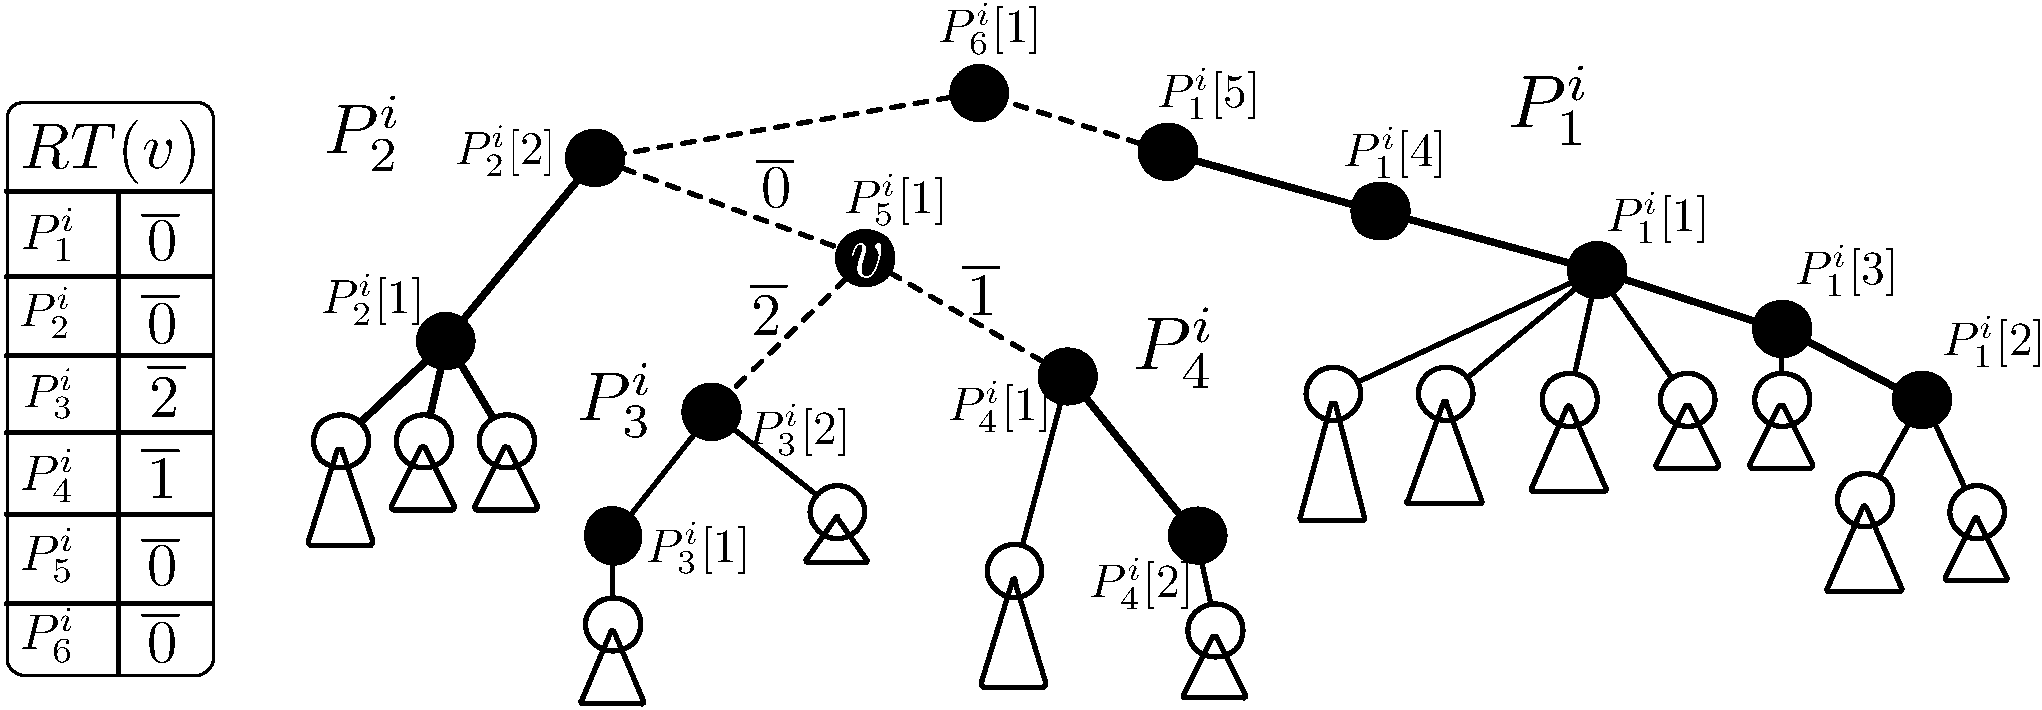
\includegraphics[width=100mm]{./Figures/Crazyrouting.pdf}
				\caption{A demonstration of naming of the  paths and $heavy_s$ nodes on level $i$ of a spines decomposition of a  subtree. 
				The thick lines are $heavy_s$ paths. The $heavy_s$ nodes are full, the $light_s$ nodes are empty, and the triangles are represent  subtrees of $light_s$ nodes.  The routing table of node $v$ to the left describes which one of the ports $\bar{0},\bar{1}$ and $\bar{2}$ it needs to traverse to arrive at nodes at other $heavy_s$ paths on level $i$. The $i$'th triplet in $\la(v)$ is $\tuple{5,1,\epsilon}$.}
				\label{fig:routing-crazy}
			\end{figure}
			

A node $v$ is assigned a two part label $\la(v)= (\Id(v),RT(v))$, described below.
The part $\Id(v)$ is, by itself, a  concatenation of triplets  of the form $\tuple{j_i,k_i,p_i}$, for $ 1 \leq i \leq  \LD(v) \leq \log_b n$, defined as follows:
 The parts $j_i$,  and $k_i$  specify $P^i_j[k]$, the $heavy_{s}$ node on level $i$ on the path  $r \leadsto v$ of maximal depth.
 We use Lemma~\ref{lemma:Gilbert} to number both $j_i$ and $k_i$.
 More specifically,  we choose  $j_i$ according to the relative contribution of  $\lsize_s(P^i_j)$ to   $\lsize_s(P^i)$, such that  $\vert j_i \vert = \log (\lsize_s(P^i)/ \lsize_s(P^i_j)) + 1$. Similarly, we choose $k_i$ according to the relative contribution of $\lsize(P^i_j[k])$ to $\lsize_s(P^i_j)$.
The part  $p_i$ is the port number used from $P^i_j[k]$ to the node $v$, which is also assigned using Lemma~\ref{lemma:Gilbert} with $\size(p_i)$ and $\lsize(P^i_j[k])$.
Note that  for the last triplet in $\Id(v)$ we use the empty string for  $p_{\LD(v)}$. 
As in Section~\ref{section:routing-intro}, the ports to  the root and the $heavy_s$ child are marked $0$ and $1$, respectively.
 Each label contains up to $\log_b n $ triplets of  three parts, where each part may be of different length.
In order to distinguish between the parts of each triplet, we store each part in $\Id(v)$ using  the suffix  code $code_1$ (see Section~\ref{sec:efficient-encoding}).
In this way a part of $m$ bits requires $m + O(\log m )$ bits, and the different parts may be concatenated.

The second part of $\la(v)$, is the level \routing table $RT(v)$ of $v$ that  contains the  ports  $v$ must use  to arrive at each of the  $heavy_{s}$ paths $P^{\LD(v)}_1 \dots P^{\LD(v)}_l$ in $v$'s level $\LD(v)$.
If $v$ is not the last node on its heavy path, then each  description concludes in traversing the path in some direction, i.e., up or down.
If $v$ is the last node, we assign the associated ports with the numbers of the ports leading to the roots of other paths in level $\LD(v)$.
This concludes the description of the label.

To compute the size of this labeling scheme we first prove the following Lemma.
\begin{lemma}\label{lemma:tikun}
$\sum_{i=1}^{\log_b n} \vert j_i \vert + \vert k_i \vert + \vert p_i \vert = \log n + O(\log_b n).$
 \end{lemma}
 
 \begin{proof}
 Let  $\tuple{j_1,k_1,p_1}$ be the first triplet in $Id(v)$ for a node $v$, and let $u$ be the light   child of  $P^1_j[k]$ to which port $p_1$ is addressed to.
  We first prove that $$\vert j_1 \vert + \vert k_1 \vert + \vert p_1 \vert \leq  \log n - \log (\size(u))+ O(1).$$
  By definition: 
  $$\vert j_1 \vert  \leq \log (n/\lsize_s(P^1_j)) +O(1) = \log n - \log (\lsize_s(P^1_j))+O(1),$$ and also 
    $$\vert k_1 \vert  \leq \log (\lsize_s(P^1_j) /\lsize_s(P^1_j[k]))+O(1) = \log (\lsize_s(P^1_j)) - \log(\lsize_s(P^1_j[k]))+O(1). $$
    Similarly, 
    $$ \vert p_1 \vert \leq \log( \lsize_s(P^1_j[k]) / \size(u) ) +O(1) =  \log( \lsize_s(P^1_j[k])) - \log (\size(u)) +O(1).$$
    Summing those inequalities we get:
    $$\vert j_1 \vert + \vert k_1 \vert + \vert p_1 \vert \leq  \log n - \log (\size(u))+ O(1),$$ as requested.
    
    Since $\lsize_s(P^2) \leq \size(u)$, we can repeat the argument so that for $w$, the light child of $P^2_j[k]$ addressed  by port $p_2$ we have:
     $$\vert j_2 \vert + \vert k_2 \vert + \vert p_2 \vert \leq  \log (\size(u)) - \log (\size(w))+ O(1).$$
     
     Summing over all the triplets, it follows that:
     $$\sum_{i=1}^{\LD(v)} \vert j_i \vert + \vert k_i \vert + \vert p_i \vert  \leq \log n +O(1) \cdot \LD(v) \leq \log n + O(\log_b n).$$
 \end{proof}

\begin{lemma} \label{lemma:routingsize}
The encoder described above produces labels of size at most $\log n + O(\log n  / \log \log n \cdot \log \log \log n)$.
\end{lemma}
\begin{proof}
 Choosing $b = \ceil{ \sqrt{\log n } }$ we can bound  the number of the  triplets  in $\Id(v)$ by  $\log_b{n} =  \frac{\log \log n}{2}$.
 The number of bits required to represent them is:
 $$\sum_{i=1}^{\log_b n} \vert j_i \vert + \vert k_i \vert + \vert p_i \vert  +O ( \sum_{i=1}^{\log_b n} \log (\vert j_i \vert)  + \log (\vert k_i \vert)  +  \log( \vert p_i \vert ) +3  ) .$$
The first sum corresponds to  the number of bits required to store the information, and the second sum is the additive number of bits required to encode each part in $code_1$. By Lemma~\ref{lemma:tikun} the first sum is bounded by  $\log n + O(\log_b n)$ bits. 
 
For brevity, we denote the number of parts by  $k= 3 \log_b n$ and the size of the $k$ parts in $\Id(v)$  by $c_1 \dots c_{3{k}}$
 Next we   bound $\sum_{i=1}^{k} \log c_i$, where $\sum_{i=1}^{k}c_i \leq  \log n + O(k)$ by Lemma~\ref{lemma:tikun}.
Since $\log$ is a concave function, we have:
$$\sum_{i=1}^{k} \log c_i \leq  k \log (\frac{\sum_{i=1}^{k} c_i}{k}) = k \log (\frac{ \log n + O(k)}{k}) \leq k \log (\frac{ \log n}{k}) +O(1)k .$$
Since $\frac{\log n}{3 \log_b n}  = \frac{\log_2 b}{3}$ the expression  can be bounded by  $O( k \log \log b+ 3 \log_b n)$, which is bounded by $O(\frac{\log n}{\log \log n}\log \log \log n).$
 

%We now prove that the $\vert RT(v) \vert $ is also $O(\log n  / \log \log n \cdot \log \log \log n)$.
To account for the size of $RT(v)$, recall that at every level of the spines decomposition there can be at most $2b-1$ paths.
Furthermore, since the ports stored lead to subtrees with at least $n/b$ nodes, it is guaranteed that each  port will be assigned an identifier with $O(\log b)$ bits. Thus, storing $RT(v)$ requires  $O( b \log b)$ bits, and  for $b = \ceil{\sqrt {\log n}}$, this can also be bounded by   $O(\frac{\log n \cdot \log \log \log n }{ \log \log n})$.
\end{proof}	 		


\paragraph{Decoding} We confirm that the information stored in the label is sufficient to determine the function \routing.
 A key observation is that while  it is not possible to  determine the rank of the a node  in its $heavy_s$ path,
 the order between two nodes on the same $heavy_s$  path can be determined.
 
Let $v$,$u$ be two nodes in $T$ with labels $\la(v) = (\Id(v),RT(v))$, $\la(u)= (\Id(u),RT(u))$ with depth  $\LD(v)$, $\LD(u)$, respectively in the recursive decomposition of $T$.
 
 If $\vert \Id(v) \vert  < \vert \Id(u) \vert $ then the decoder returns $0$, since that implies that $u$ is not an ancestor of $v$ and the path $u \leadsto v$ must begin with the edge traversing upwards from $u$.
Using the same argument,  we  return $0$ if the first $\LD(u)-1$ triplets of both $\Id(v)$ and $\Id(u)$ are not equal.
 
 Let $(path_v,node_v,edge_v)$ and $(path_u,node_u,\emptystring)$ be   triplets number $\LD(u)$ in $\Id(v)$ and $\Id(u)$, respectively.
There are three possible scenarios:
\begin{itemize}
	\item If $path_v = path_u$ and $node_v = node_u$ return $edge_v$.
	\item If $path_v = path_u$ and $node_v \neq node_u$, then determine which of $node_v$ and $node_u$ are first on the heavy path and return $0$ if the former and $1$ if the latter.
	\item If $path_v \neq path_u$ then return the edge corresponding to the traversal from $path_u$ to $path_v$ in  $RT(u)$.
\end{itemize}

		
Lemma~\ref{lemma:tikun} is a  correction to Lemma 2.4 in the  original proof in~\cite{Thorup01}.
Using similar definitions, the Lemma argues that every triplet requires at most $\log b +2$ bits. 
The term $\lsize_s(\overline{\overline{v}})$ represents the size of the subtree rooted in a  $light_s$ node at any level including the first, and  therefore  $1\leq \size(\overline{\overline{v}}) \leq n/b$. From that we get that $\log_2 \frac{n}{\lsize_s(\overline{\overline{v}})}+2 > \log_2 b +2$.
In fact the claim $\log_2 \frac{n}{\lsize_s(\overline{\overline{v}})}+2 \leq \log_2 b +2$  in~\cite{Thorup01}  holds in the opposite direction. 

 
\paragraph{Implications}		
From  this upper bound  and the recent lower bound for \NCA~\cite{Green14} it follows that any labeling scheme for \NCA is of  provably larger size than the size required for \routing.
The question of whether  the best possible lower order term is  $O(\log n / \log \log n)$ or  $O(\log \log n)$ remains open. 
The current lower bound for designer port \routing in trees stands at $\log n + O (\log \log n)$. This follows from its relationship to \ancestry labeling schemes reported earlier. Clearly, it is of great interest to prove that a larger label size is needed for \routing  than needed for  \ancestry/\siblings/\connectivity labeling schemes.


\subsection{Fixed Port Model}\label{sec:ThorupZwickFixedPort}
We now consider the fixed port  model, i.e  the model where the port numbers are chosen by an adversary. 
We provide a proof of the following result of~\cite{Thorup01} that was omitted in their paper.
\begin{theorem} \label{thm:routing-upper-fixed}  	
	There exist a fixed  port model \routing labeling scheme for $Trees(n)$, denoted  $\tuple{e,d}$, with labels of size at most $O(\log^2 n / \log \log n)$.
\end{theorem}
\begin{proof}
	The encoder operates on the tree $T$  similarly to the one for the designer port problem.
		A node $v \in T$ with label $(\Id(v),RT(v))$ is transformed in the following manner:
		We store  additional  $\log n$ bits to denote the port number assigned by the adversary to the edge in each triplet in $\Id(v)$.
		Recall that the \routing table $RT(v)$ contains at most $b$ port numbers. We store the edge numbering  assigned by the adversary for each entry in the table.
		The new $\Id(v)$ requires  additional $\log n$ bits for each of the $\log_b n$ parts, and the new $RT(v)$ requires $b  \log n$ additional bits.  Setting $b= \ceil{ \sqrt{ \log n}}$ as before,  the total new label length is bounded by $O(\log^2 n / \log \log n)$, as required.	
\end{proof}

The labeling scheme in Theorem~\ref{sec:ThorupZwickFixedPort} is asymptotically optimal in light of  the lower bound in \cite{fraigniaud2002space}. An alternative proof for the existence  of such a labeling scheme is  given in~\cite{Fraigniaud01}.



%\paragraph{Upper bound}
%
%
%\paragraph{Lower bound}
%Fraigniaud and Gavoille proved that any labeling scheme supporting the function is of size $\Omega(\log^2 n / \log \log n)$.
%More specifically, they construct a family of trees and define a relaxed query for which the bound still holds.
%The authors consider a full k-ary tree, where $k= (\log \sqrt n / \log \log \sqrt n)-1$ and  every internal node has $\sqrt n$ leaves attached, where the height of the tree is  $h = \log \sqrt n / \log \log \sqrt n$. 
%The proof is inductive over a series of k-ary trees over varying $h$, and decreasing number of leaves per node.
%
%A key observation is that once the port assignment of the ports from the root is set, no two trees can have the exact same labels.

%The authors show that $\la^t$ 






	



	
%% !TEX root = ../Survey.tex
\section{Labeling Schemes for Dynamic Tree Networks }\label{section:dynamic}
The labeling schemes described so far assume the existence of a tree of $n$ nodes. In real life applications, such tree is not known in advance. When the topology of the tree and its size undergo repeated changes a different method is required.
We describe  general dynamic labeling schemes. By that we mean  a method to extend an existing \emph{static} labeling scheme for the dynamic setting.
		
		
We adopt the terminology in~\cite{korman2004labeling}, which names dynamic encoding algorithms as \emph{distributed online protocols} or simply \emph{protocols}.
The following types of topology changes are considered:
	\begin{inparaenum}[\itshape a\upshape)]
			\item \emph{Add-Leaf}, where a new degree-one node $u$ is added as a child of an existing node $v$
			; and \item \emph{Remove-Leaf}, where a  (non-root) leaf $v$ is deleted.
	\end{inparaenum}
Dynamic labeling schemes that support only \emph{Add-Leaf} are denoted  \emph{semi-dynamic}, and those that support both operations are denoted  \emph{fully-dynamic}.

\textbf{Metrics  for dynamic labeling schemes.} In the literature surveyed, labeling schemes aim for smallest label possible.
If communication is not accounted for, dynamic labeling schemes can trivially achieve the optimal, static bounds.
Therefore, in order to account for the cost of communication, the following  metrics are introduced~\cite{korman2004labeling}.
Let $M$ be a dynamic labeling scheme, with re-labeling allowed, and let $S(n)$ be a sequence of $n$ topological changes.
\begin{enumerate}
	\item \emph{Message Complexity}, $\MC(M, n)$: the maximum number of messages sent in total by $M$ on $S(n)$. Messages are sent  exclusively between adjacent  nodes.
	\item \emph{Bit Complexity}, $\BC(M, n)$: the maximum number of bits sent in total by $M$ on $S(n)$.
	\item \emph{Label Size} $\LS(M,n)$:  the maximum size of a label assigned by $M$ on $S(n)$.
\end{enumerate}

\begin {table}
	\begin{center}
	    \begin{tabular}{ | l | l | l | l |}
		    \hline
		    Labeling Scheme & Label Size & $\MC$ & $\BC$ \\ \hline
		    \emph{Distance} 	&$O(\log^2 n)$ & $O(n)$ & $O(n \log^2 n)$ \\ \hline
		   SemDL	&$O(\log^2 n)$ & $O(n \log^2 n)$ & $O(n \log^2 n \log \log n)$  \\ \hline
		    DL 		&$O(\log^2 n)$ & $O(n \log^2 n$) & $O(n \log^2 n \log \log n)$ \\ \hline
		   SemGL	&$O(\frac{d-1}{\log d}\log^3 n)$ & $O(n \frac{\log n}{\log d})$ & unreported   \\ \hline
		    GL		& $O(\log^3 n)$ & $O(n \log^2 n)$ & unreported \\
		    \hline
	    \end{tabular}
	 \end{center}
	 	\caption{Simplified complexity estimates for $Trees(n)$. Bounds for $GL$  are reported with $d=2$. See~\cite{korman2004labeling} for an elaborate complexity report.}
	\label{table:complexities}
\end{table}
				
Korman et al.~\cite{korman2004labeling} presented \emph{semi-dynamic} and  \emph{fully-dynamic}  labeling schemes that support distance queries and  a \emph{semi-dynamic} and \emph{fully-dynamic}  labeling scheme that, under conditions, receives a static labeling scheme as input and supports queries of its type. To the best of our knowledge, none of the static labeling schemes in the literature fail to obey the conditions.

 We denote the static distance labeling scheme as  \emph{Distance}, its extension to a specialized  semi-dynamic mode  \emph{SemDL}, and its fully-dynamic  specialized extension as \emph{DL}. 
Korman et al.~\cite{korman2004labeling} define the general dynamic labeling schemes \emph{SemGL} and \emph{GL}, which maintain labels on each node of a dynamically changing tree network using a static labeling scheme as a subroutine. The performance of these schemes is tightly coupled to the performance of the static scheme used.
 Throughout the remainder, we denote the general labeling schemes operating on \emph{Distance} simply as \emph{SemGL} and \emph{GL}, and explicitly mention other distance functions where appropriate.  
 Table~\ref{table:complexities}  reports the  different  complexities  for the aforementioned schemes (the parameter $d$ is explained later).



\textbf{SemDL.}
The protocol extends the distance labeling scheme explained in Theorem~\ref{thm:nca-designer-long}, based on the heavy-light decomposition.
 It is not essential for the correctness of the decomposition that the heavy node selected be in fact the heaviest, or say, the 3rd largest. It is only essential for the bound on the label size.
SemDL maintains a dynamic version of the sketched labels using this exact observation. Every node maintains an estimate of its weight, and transfers this estimate to its parent, using a previously introduced binning method~\cite{afek1996local}.
When the estimate exceeds a threshold in a node, this implies that a node other than the heavy node is now significantly heavier than the heavy node. Thus, a  re-labeling (shuffle, in~\cite{korman2004labeling}) is instantiated on the subtree to maintain the $O(\log^2 n)$ label size.
%There are two types of messages passed across the tree network: labeling, and bin messages.

\textbf{SemGL.} The protocol is designed to transform any static labeling scheme $Static$ to semi-dynamic, and therefore, does not utilize the heavy-light decomposition directly.
Instead, the protocol operates $Static$  separately on a cleverly constructed sets of bubbles described hereafter.

Each node $v \in T$ is included in exactly one induced subtree of $T$, denoted  \emph{bubble} of \emph{order} $i$ ($0 \leq i \leq \log_d n$) that  contains at least   $d^i$  nodes. 
The bubbles constitute a  \emph{bubble tree}, where the order of  a bubble is always less or equal to the order of the parent bubble. 
 In addition, there are no $d$ consecutive bubbles of the same order in any path of the bubble tree. 
A node added to the tree is assigned the order $0$. If this insertion yields $d$ consecutive bubbles of order $0$ in the bubble tree, they are merged to a single  bubble of order $1$, and the condition is checked again for bubbles of order $1$ and so on. We denote the parent of the root of  bubble $b$ as $b_p$ and the function that $Static$ supports as $f$.
 Essentially, the label of a node $v$ in a bubble $b$ is a concatenation of the label of $b_p$ with both   a local $Static$ label of $v$ in $b$, and the result of $f(v,b_p)$.  
 
\textbf{Semi-dynamic to fully-dynamic conversion.} Both labeling schemes are converted to their counterpart fully-dynamic labeling schemes, DL and GL, using an additional simple protocol.
The protocol uses the binning method~\cite{afek1996local} to maintain local weight estimates for each node.
The protocol simply ignores the topological changes up to the point in which their number is large, and then re-labels the entire tree.



%% !TEX root = ../Survey.tex
\section{Bounded cases}\label{section:bounded-cases}
We describe the new results mentioned in table ~\ref{Table2}.
%\paragraph{Routing}
\paragraph{Ancestry}
	\begin{thm} \label{thm:cat-anc}
		 $Caterpillars(n)$ have an ancestry  labeling scheme of $ \log n + \Theta(1)$
	\end{thm}
		\begin{proof}
			 Note that in contrast to general case,  only internal vertices can be mutual ancestors.
	 		Let $I_1 \dots I_k$ be the internal vertices of the rooted caterpillar $T = (V,E)$, for each  $1 \leq i \leq k$ we mark the $k_i$ leaves of $I_i$ as $L_i^1 \dots L_i^{k_i}$.
			Let $r  \in V$ be the root of $T$. 
			The encoder assigns  each node  a number in the range $[1 \dots n]$ using a BFS scan on $T$ from $r$.
			The connected internal node is last in the scan and receives the number $k_1 +1$, and the labeling continues recursively.
			We mark internal vertices by a prefix $0$ to the label, and $1$  for a leaf.
			
			For query $Ancestor(u,v)$, the decoder can safely reject if $u$ and $v$ are leaves.
			Otherwise, the query would return true if and only if $u<v$.
		 \end{proof}
 \paragraph{Distance}
	 \begin{thm} \label{thm:cat-dist}
	 $Caterpillars(n)$ have a distance labeling scheme of $2 \log n$
	 \end{thm}
	 
	 \begin{proof}
	 Let $I_1 \dots I_k$ be the internal vertices of the caterpillar $T$, for each  $1 \leq i \leq k$ we mark the $k_i$ leaves of $I_i$ as $L_i^1 \dots L_i^{k_i}$.
	 The encoder assigns $I_i$ the label $\tuple{i,0}$ and its leaves $L_i^1 \dots L_i^{k_i}$ the labels $\tuple{i,1} \dots \tuple{i,k}$ in according.
	 Assume that $a \geq c$.
	 The decoder acts on query $Distance(\tuple{a,b},\tuple{c,d})$ as follows:
	 	\begin{enumerate}
		\item $b=d=0$ : return $a-c$
		\item $ b\neq 0 ,d \neq 0$ : return $a-c+2$ if $ a \neq c$ and $0$ otherwise.
		\item $ b = 0 ,d \neq 0$ or  $ b  \neq 0,d = 0$  : return $a-c+1$
	 	\end{enumerate}
		Since $1 \leq i,k_i \leq n$ we conclude that the latter can be decoded using (exactly) $ 2 \log n$ bits.
		Moreover, for $Caterpillars(n,\Delta)$, $k_i \leq \Delta$, and for $Caterpillars(n,\delta)$, $i \leq \Delta$.
		Thus, for both cases  only $  \log n + \log \Delta $  are required.
 	 \end{proof}
	 
	 If $T$ is an edge  weighted with maximum edge weight $2^M$ we assign  for $I_i$ with weight $w(I_i)$ the label $\tuple{\sum_{j=1}^{i} w(I_j) ,0,0}$ 
	 
	 The leaves $L_i^1 \dots L_i^{k_i}$ are assigned the labels
	 
	  $\tuple{\sum_{j=1}^{i} w(I_j) , w(L_i^1)  ,1} \dots \tuple{\sum_{j=1}^{i} w(I_j) , w(L_i^{k+1})  ,k+1} $ in according.
	  
	   Assume that $a \geq d$.
	 The decoder now  acts on query $Distance(\tuple{a,b,c},\tuple{d,e,f})$ as follows:
	 	\begin{enumerate}
		\item $c=f=0$ : return $a-d$
		\item $ c\neq 0 ,f \neq 0$ : if $\tuple{a,b,c} \neq \tuple{d,e,f}$  return $a-d+b+e$, otherwise  $0$.
		\item $ c = 0 ,f  \neq 0$ : return $a-d+e$
		\item $ c \neq  0 ,f  = 0$ : return $a-d+b$
	 	\end{enumerate}
		
		
	 \begin{corollary}\label{Cor:lowerbounds}
	 \hfill
	 \begin{itemize}
	 	\item Edge weighted $Caterpillars(n,2^M)$  have a distance labeling scheme of $2 \log n + 2M$
		\item  Edge weighted  $Caterpillars(n,\Delta,2^M)$   have a distance labeling scheme of $ \log n  + \log \Delta + 2M$
	\end{itemize}
	 \end{corollary}
%
%\paragraph{Center}
%
%	 \begin{thm} \label{thm:cat-dist}
%	 $Caterpillars(n)$ have a center  labeling scheme of $2 \log n$
%	 \end{thm}
%	 
%	 \begin{proof}
%	 
%	 \end{proof}

\paragraph{The implications of Alstrup's lower bounds on the limited variants}
The limits attained by Alstrup \cite{Alstrup05} applies directly for ancestry in the bounded depth and degree cases. The sibling bound applies  for caterpillars,  and bounded  depth trees.
As seen in Figure~\ref{fig:loubou}, the lower bound for siblings is defined for $\delta =3$. Moreover, each tree of the $\log n$ trees in the family can be transformed  to a caterpillar in the following manner.
Denote the set of nodes neighboring to the root by $v_1 \dots v_i$.  We remove the root $r$ and for each  $1 \leq  j < i$  we replace each edge $(r,v_j)$ with $(v_j,v_{j+1})$ .
The transformed  family of caterpillars  maintains  the  lower bound for sibling relation.

We can thus conclude:

	\begin{corollary}
	\hfill
	 	\begin{itemize}
		\item  Any sibling labeling scheme for $Caterpillars(n)$  must have a labeling scheme of at least  $ \log n +O(\log \log n)$ bits.
		\item	Any sibling labeling scheme for $Caterpillars(n,\delta)$ ($\delta \geq 2$)  must have a labeling scheme of  at least $ \log n +O(\log \log n)$ bits.
		\end{itemize}
	\end{corollary}

\begin{figure}
\centering
\makebox[\textwidth][c]{
\begin{tikzpicture}[thick,scale=0.4, every node/.style={scale=0.55}]

\tikzstyle{Node}=[circle,fill=White,draw=Black]

\tikzstyle{NiceNode}=[circle,fill=White,draw=Black,scale = 1,
font=\small]

\tikzstyle{Edge}=[]

\tikzstyle{NiceEdge}=[dotted]

\tikzstyle{ControlNodes} = [circle,fill=Black,draw=Black]

\tikzstyle{none}=[inner sep=0pt]
		\node [style=ControlNodes] (0) at (-9, 1.5) {};
		\node [style=NiceNode] (1) at (-10.25, 0) {};
		\node [style=NiceNode] (2) at (-9.5, 0) {};
		\node [style=NiceNode] (3) at (-7.25, 0) {};
		\node [style=ControlNodes] (4) at (-4.75, 1.5) {};
		\node [style=NiceNode] (5) at (-6, 0) {};
		\node [style=NiceNode] (6) at (-3, 0) {};
		\node [style=NiceNode] (7) at (-4.75, 0) {};
		\node [style=ControlNodes] (8) at (-7.25, 2.75) {};
		\node [style=ControlNodes] (9) at (7, 3) {};
		\node [style=ControlNodes] (10) at (4.75, 1.5) {};
		\node [style=NiceNode] (11) at (-0.75, 0) {};
		\node [style=NiceNode] (12) at (4.75, 0) {};
		\node [style=NiceNode] (13) at (2.25, 0) {};
		\node [style=ControlNodes] (14) at (0.5, 1.5) {};
		\node [style=NiceNode] (15) at (4, 0) {};
		\node [style=NiceNode] (16) at (6.5, 0) {};
		\node [style=NiceNode] (17) at (0, 0) {};
		\node [style=NiceNode] (18) at (8.5, 0) {};
		\node [style=ControlNodes] (19) at (9, 1.5) {};
		\node [style=NiceNode] (20) at (7.75, 0) {};
		\node [style=NiceNode] (21) at (13.25, 0) {};
		\node [style=ControlNodes] (22) at (13.25, 1.5) {};
		\node [style=NiceNode] (23) at (15, 0) {};
		\node [style=NiceNode] (24) at (10.75, 0) {};
		\node [style=NiceNode] (25) at (12.5, 0) {};
		\node [style=NiceNode] (26) at (-15, 0) {};
		\node [style=NiceNode] (27) at (-12, 0) {};
		\node [style=ControlNodes] (28) at (-13.75, 1.5) {};
		\node [style=NiceNode] (29) at (-14.25, 0) {};
		\node [style=ControlNodes] (30) at (-13.75, 2.75) {};
		\node [style=ControlNodes] (31) at (1.75, -1) {};
		\node [style=NiceNode] (32) at (5.25, -3.5) {};
		\node [style=ControlNodes] (33) at (3, -2.25) {};
		\node [style=NiceNode] (34) at (3.75, -3.5) {};
		\node [style=NiceNode] (35) at (1.5, -3.5) {};
		\node [style=NiceNode] (36) at (6.5, -3.5) {};
		\node [style=ControlNodes] (37) at (5.75, -2.25) {};
		\node [style=NiceNode] (38) at (0.75, -3.5) {};
		\node [style=NiceNode] (39) at (0, -3.5) {};
		\node [style=ControlNodes] (40) at (1.75, -2.25) {};
		\node [style=ControlNodes] (41) at (0.75, -2.25) {};
		\node [style=NiceNode] (42) at (3, -3.5) {};
		\node [style=NiceNode] (43) at (2.25, -3.5) {};
		\node [style=NiceNode] (44) at (15, -3.5) {};
		\node [style=ControlNodes] (45) at (11, -1) {};
		\node [style=ControlNodes] (46) at (15, -2.25) {};
		\node [style=NiceNode] (47) at (11, -3.5) {};
		\node [style=ControlNodes] (48) at (10, -2.25) {};
		\node [style=ControlNodes] (49) at (11, -2.25) {};
		\node [style=ControlNodes] (50) at (12.25, -2.25) {};
		\node [style=NiceNode] (51) at (12.25, -3.5) {};
		\node [style=NiceNode] (52) at (10, -3.5) {};
		\node [style=NiceNode] (53) at (-14.75, -3.5) {};
		\node [style=ControlNodes] (54) at (-13.5, -2.25) {};
		\node [style=ControlNodes] (55) at (-8.75, -1) {};
		\node [style=NiceNode] (56) at (-13, -3.5) {};
		\node [style=NiceNode] (57) at (-14, -3.5) {};
		\node [style=NiceNode] (58) at (-12.25, -3.5) {};
		\node [style=NiceNode] (59) at (-10.75, -3.5) {};
		\node [style=NiceNode] (60) at (-11.5, -3.5) {};
		\node [style=ControlNodes] (61) at (-10.25, -2.25) {};
		\node [style=NiceNode] (62) at (-9, -3.5) {};
		\node [style=NiceNode] (63) at (-9.75, -3.5) {};
		\node [style=NiceNode] (64) at (-5.75, -3.5) {};
		\node [style=ControlNodes] (65) at (-7, -2.25) {};
		\node [style=NiceNode] (66) at (-8.25, -3.5) {};
		\node [style=NiceNode] (67) at (-7.5, -3.5) {};
		\node [style=NiceNode] (68) at (-6.5, -3.5) {};
		\node [style=NiceNode] (69) at (-2.5, -3.5) {};
		\node [style=ControlNodes] (70) at (-3.75, -2.25) {};
		\node [style=NiceNode] (71) at (-5, -3.5) {};
		\node [style=NiceNode] (72) at (-4.25, -3.5) {};
		\node [style=NiceNode] (73) at (-3.25, -3.5) {};
		\draw (0) to (1);
		\draw (0) to (2);
		\draw (0) to (3);
		\draw [style=NiceEdge] (2) to (3);
		\draw (4) to (5);
		\draw (4) to (7);
		\draw (4) to (6);
		\draw [style=NiceEdge] (7) to (6);
		\draw (0) to (8);
		\draw (8) to (4);
		\draw (14) to (11);
		\draw (14) to (17);
		\draw (14) to (13);
		\draw [style=NiceEdge] (17) to (13);
		\draw (10) to (15);
		\draw (10) to (12);
		\draw (10) to (16);
		\draw [style=NiceEdge] (12) to (16);
		\draw (14) to (9);
		\draw (9) to (10);
		\draw (19) to (20);
		\draw (19) to (18);
		\draw (19) to (24);
		\draw [style=NiceEdge] (18) to (24);
		\draw (22) to (25);
		\draw (22) to (21);
		\draw (22) to (23);
		\draw [style=NiceEdge] (21) to (23);
		\draw [style=Edge] (9) to (19);
		\draw [style=Edge] (9) to (22);
		\draw (28) to (26);
		\draw (28) to (29);
		\draw (28) to (27);
		\draw [style=NiceEdge] (29) to (27);
		\draw (28) to (30);
		\draw (41) to (39);
		\draw (41) to (38);
		\draw (40) to (35);
		\draw (40) to (43);
		\draw (41) to (31);
		\draw (31) to (40);
		\draw (33) to (42);
		\draw (33) to (34);
		\draw (37) to (32);
		\draw (37) to (36);
		\draw [style=Edge] (31) to (33);
		\draw [style=Edge] (31) to (37);
		\draw [style=NiceEdge] (33) to (37);
		\draw (48) to (52);
		\draw (49) to (47);
		\draw (48) to (45);
		\draw (45) to (49);
		\draw (50) to (51);
		\draw (46) to (44);
		\draw [style=Edge] (45) to (50);
		\draw [style=Edge] (45) to (46);
		\draw [style=NiceEdge] (50) to (46);
		\draw (54) to (53);
		\draw (54) to (56);
		\draw (54) to (55);
		\draw [style=Edge] (54) to (57);
		\draw [style=Edge] (54) to (58);
		\draw (61) to (60);
		\draw (61) to (63);
		\draw [style=Edge] (61) to (59);
		\draw [style=Edge] (61) to (62);
		\draw (65) to (66);
		\draw (65) to (68);
		\draw [style=Edge] (65) to (67);
		\draw [style=Edge] (65) to (64);
		\draw (70) to (71);
		\draw (70) to (73);
		\draw [style=Edge] (70) to (72);
		\draw [style=Edge] (70) to (69);
		\draw [style=Edge] (55) to (61);
		\draw [style=Edge] (55) to (65);
		\draw [style=Edge] (55) to (70);
		\draw [style=NiceEdge] (65) to (70);
		
\end{tikzpicture}
}
\caption{The 3 first (First line)  and 3 last  (Second line)  members of the  family of trees introduced for the siblings lower bounds} \label{fig:loubou}
\end{figure}


 

\bibliographystyle{ACM-Reference-Format-Journals}
\bibliography{lit}
\elecappendix

\medskip
\section{Basic Definitions}\label{AppendixA}
% !TEX root = ../Survey.tex
%If $u$ is a node on the path from the root of a rooted tree to a node $v$, then $u$ is an \emph{ancestor} of $v$, and $v$ is a \emph{descendant} of $u$. If, in addition, $\depth(v)=\depth(u)+1$ so that $uv$ is an edge, then $u$ is the unique \emph{parent} of $v$, denoted $\parent(v)$, and $v$ is a \emph{child} of $u$. Two nodes that have the same parent are \emph{siblings}. Note, in particular, that a node is its own ancestor, descendant and sibling, but not its own child or parent. A \emph{common ancestor} of two nodes is a node that is an ancestor of both nodes, and their \emph{nearest common ancestor} (NCA) is the unique common ancestor with maximum depth. Given a node $v$, the descendants of $v$ form an induced subtree $T_v$ with $v$ as root. 
%
%A \emph{binary tree} is a rooted tree in which all nodes have at most two children. A binary tree $T$ is \emph{full} if all internal nodes have exactly two children and is \emph{complete} if there are exactly $2^i$ nodes with depth $i$ for all $i<d$, where $d$ is the depth of the tree. A binary tree that is both full and complete and where all leaves are at the same depth is \emph{perfect}. A perfect binary tree will have $2^i$ nodes of depth $i$ for all $i\leq d$ and a total of $2^{d+1}-1$ nodes, whereof $2^d$ are leaves. A \emph{star} is a tree in which all nodes but one are leaves.
%
%
%	\begin{definition}\label{dfn:tree-things-app}
%	Let $T=(V,E)$ be a connected acyclic undirected graph, in other words, a \emph{tree}.
%	 The number of edges in a tree is always $|E|=|V|-1$, and every two nodes are connected by a unique path.
%	A tree may contain a speciallnodey designated node called the \emph{root}, in which case the tree is \emph{rooted}. The nodes of degree $1$ other than the root are called \emph{leaves}, and all other nodes are called \emph{internal} nodes. The distance from a node $v$ to the root is called the \emph{depth} of $v$, denoted $\depth(v)$. 
%The depth of the tree, $\depth(T)$, is the maximum depth among the nodes in $T$. 
%	The number of edges in a tree is always $|E|=|V|-1$, and every two nodes are connected by a unique path.
%	
%		The rooted \emph{forest}  $F =(V_F,E_F)$ is  a collection of  rooted trees.
%
%	\begin{enumerate}
%		\item The vertices $v,u \in V$ are \emph{neighbours} if $(v,u) \in E$. The set of all neighbours of $v$ is labeled $N(v)$.
%		\item A  node $v \in V$ has a \emph{degree} $k$ if it has $k$ neighbours, $deg(v)=k$.
%		\item A  node $v \in V$ that has  a degree of at most 1 is called a  \emph{leaf}, and an \emph{inner node} is a non-leaf node.
%		\item A \emph{path} of \emph{length} $k$ from a node $v$ to a node $u$ in a graph $G=(V,E)$  (denoted $v \leadsto u$) is a sequence  \tuple{v_0,v_1 \dots v_k} of vertices such that $v = v_0$, $u = v_k$, and $(v_{i-1},v_{i})\in E$ for $ i= 1,2 \dots k$.
%		\item Let $v,u \in V_F$. The distance between $u$ and $v$ in $F$, denoted $dist_F (u, v)$, is the number of edges on the path  $u \leadsto v $. If $u$ and $v$ are not in the same tree in $F$, the function returns $\infty$.
%		\item We denote for  each $v \in V$  $depth(v)= dist_T (v, r)$. 
%		\item Let $v,u \in V$, we denote  the parent of $u$ by $p(u)$. A \emph{sibling} $(v \neq u$ of $u)$  is a child of   $p(u)$. 
%		\item Let $v,u \in V$, we say that $u$ is a \emph{child} of $v$ if $u \in N(v)$ and $v$ is the root, and  $u \in N(v)-p(v)$ if $v$ is not the root. We label  all children of node $v$ as $Children(v)$.
%		\item The \emph{size} of $v \in V$, $\vert v \vert $, is the number of nodes in $T_v$: that is, the number of descendants of $v$.
%		\item The \emph{weighted diameter} of $T$,denoted $dist(T)$,  is defined as the maximum distance in $T$; that is $dist(T) =  \max_{x,y \in V}  dist_T (u, v)$
%		\item We say that $T$ is \emph{$2^M$ edge weighted} if for each $e \in E$ we assign  an integer  $1 \leq w(e) \leq 2^M$.
%
%	\end{enumerate}
%	\end{definition}

\subsection{Sets and Operations}
	\begin{definition}
	Let $A$ and $B$ be languages. We define the regular operations \emph{union}, \emph{intersection}, and \emph{star}
	as follows:
	\begin{enumerate}
		\item Union: $ A \cup B = \{ x \vert x \in A \text{ or } x \in B \} $.
		 \item Intersection:  $ A \cap B = \{ x \vert x \in A \text{ and } x \in B \} $.
		\item Star:  $ A^* = \{ x_1x_2\dots x_k \vert k \geq 0 \text{ and each } x_i \in A \} $.
	\end{enumerate}
	\end{definition}

\subsection{Universal graphs}
The definitions are from \citeN{Kannan92}.
		\begin{definition} \label{dfn:node-induced}
			A node induced subgraph or simply an induced subgraph $G'$ of $G$ is a node set $V' \subseteq V$ together with the edge set $E' = E \cap (V' \times V')$.
		\end{definition}
		\begin{definition} \label{dfn:universal}
			Given finite set of graphs $\mathcal{G}$, a graph $G$ is node induced universal for  $\mathcal{G}$ if every graph in $\mathcal{G}$ is a node induced subgraph of $G$.
			We say that a family $\mathcal{F}$ has universal graphs of size $g(n)$ if for every $n$ there is a graph of size less than or equal to $g(n)$ which is node induced universal for 	the set of all graphs in $\mathcal{F}$
			with $n$ or fewer vertices.
		\end{definition}
			
\subsection{Probability}
\begin{definition}\label{dfn:prob}
	The definitions  are cited from \citeN{Cormen01}.
	
	 A sample space $S$ is a set of \emph{elementary events}.
	An \emph{event} is a subset of the sample space $S$.
	Events $A$ and $B$ are mutually exclusive if $ A \cap B = \emptyset $
	A \emph{Probability distribution} $prob()$ on a sample space $S$ is a mapping from events of $S$ to real numbers satisfying the following \emph{probability axioms}:
	\begin{enumerate}
		\item $prob(A) \geq 0$ for any event $A$.
		\item $prob(S) = 1$
		\item $prob(A \cup B) =prob(A)+ prob(B)  $ for any two mutually exclusive events $A$ and $B$.
	\end{enumerate}
	
	A random variable is a function from $S$ into the real numbers.
	
	For a random variable $X$ and a real number $x$, we define the event  $X = x$ to be $\{ s \in S : X(s) = x \}$; thus,
	$$ prob(X=x)  = \sum_{s \in S:X(s)=x} prob(s)$$
	
	The expected value (or, synonymously, expectation or mean) of a discrete random variable $X$ is:
	$$EX=\sum_{x} x \cdot prob(X=x)$$
	
	\end{definition}

\section{Proof of the claim in  Lemma~\ref{Lemma-adj-loglogn}}\label{AppendixB}
% !TEX root = ../Survey.tex
Consider the non-leaf  node $v$ with parent $p(v)$ and heavy child $h(v)$ in a rooted tree $T$.
 Recall that the encoder of $\tuple{e_\alpha,d_\alpha}$ labels $v$ as a concatenation of  the bit strings:
\begin{inparaenum}[\itshape I.\upshape)]
  \item{$\dfsi(v)$};
 \item $\ldepth(v)$;
 \item a $1/2$-approximation of $\dfsi(v)-\dfsi(p(v))$; and
 % denoted $\lfloor o \rfloor_2(v)$
\item~a $1/2$-approximation of $\dfsi(h(v))-\dfsi(v)$.
  %denoted $\lfloor ls \rfloor_2(v)$.
 \end{inparaenum}
 

\newcommand{\recomp}{\operatorname{recomp}}
\newcommand{\pprox}{\lfloor P \rfloor _2}
\newcommand{\cprox}{\lfloor C \rfloor _2}


 We denote the $1/2$-approximation of $\dfsi(v)-\dfsi(p(v))$  as $\pprox(v)$  and  and  the $1/2$-approximation of $\dfsi(h(v))-\dfsi(v)$ as $\cprox(v)$.
 The decoder receives both labels $\la(u)$ and $\la(v)$ and  computes the value  $\recomp(u,v)$ which takes a $1/2$ approximation of the values 
 $\dfsi(u)-\dfsi(v)$ given by their labels.
 
 

Suppose  $u$ is  the  parent of the node   $v$.
The decoder  $d_\alpha$ returns true for  $\la(u),\la(v)$ by verifying  the following predicates hold:
\begin{itemize}
\item $\dfsi(u)< \dfsi(v)$.
\item $\ldepth(v) = \ldepth(u)$ if $v$ is heavy, and $\ldepth(v) = \ldepth(u)+1$ if $v$ is light.
\item  $ \cprox(u) = \pprox(v)  $ if $v$ is heavy and $ \cprox(u) \geq \pprox(v)  $ if $v$ is light.
\item   $\recomp(u,v) =  \pprox(v)$.
\end{itemize}

 The above conditions are clearly sufficient if $u$ is the parent of $v$.
 We now denote the heavy child of $u$ as $h(u)$.
Assume in contradiction that the conditions hold, but $u$ is not the parent of  the node $v$. 
First, assume that $v$ is light. 
The first  two predicates assure that $u$ can not be a descendant of $v$. 
Since $v$ has $\ldepth(u)+1$ it must be the child of either of $h(u)$ or not a decedent of $v$ at all.
In both cases the path $u \leadsto v$ must contain at least one more node $y= p(v)$ where $\dfsi(y) \geq \dfsi(h(u))$.
It follows that : 
\begin{equation}\label{eq:yep}
\dfsi(v)-\dfsi(u) \geq  \dfsi(v)- \dfsi(y) + \dfsi(h(u))- \dfsi(u) \geq 2 min(\cprox(u),\pprox(v)).
\end{equation}
Since $v$ is light we know that:
$$\cprox(u) \geq \pprox(v) = \recomp(u,v).$$
It follows that  $\recomp(u,v) = min(\cprox(u),\pprox(v))$, and since $\recomp$ is a $1/2$-approximation:
 $$2 \recomp(u,v) =  2 min(\cprox(u),\pprox(v)) > \dfsi(v)-\dfsi(u),$$
 which is a contradiction.
 
 If $v$ is heavy, it may no longer be a decedent of $u$, and there exist a $y = p(v)$ for which equation~\ref{eq:yep} holds as before, and the contradiction holds similarly.  

\newpage
\section{Proof of the claim in  Section~\ref{traversaljumping}}\label{AppendixC}
 % !TEX root = ../Survey.tex

  The proof follows directly from the following lemma.
 \begin{lemma}
The  following property holds for every $2 \leq m \leq p$ for some constant $c'$:
 $$\sum_{i=m}^p 2^{t_i} \leq c' \sum_{i=m}^p \lceil l(i) \rceil_2 - 2^{t_m}.$$
 \end{lemma}
 \begin{proof}
 We prove this claim by induction over $m$ from $p$ down to $2$. The claim holds trivially for $m=p$.
 Assume that the property holds for $m$, for $m-1$ by the induction hypothesis:
 $$\sum_{i=m-1}^p 2^{t_i} \leq c' \sum_{i=m}^p \lceil l(i) \rceil_2 - 2^{t_m} + 2^{t_{m-1}}.$$
 If  $\lceil l(m-1) \rceil_2 \geq 2^{t_m}$ then $2^{t_{m-1}} = \lceil l(m-1) \rceil_2$ by definition, and thus for $c'>2$:
  $$\sum_{i=m-1}^p 2^{t_i} \leq c' \sum_{i=m}^p \lceil l(i) \rceil_2 - 2^{t_m} + 2^{t_{m-1}} =  c' \sum_{i=m-1}^p \lceil l(i) \rceil_2 - 2^{t_m} - (c'-1) \lceil l(m-1) \rceil_2 \leq c' \sum_{i=m-1}^p \lceil l(i) \rceil_2  - 2^{t_{m-1}}.$$
If $\lceil l(m-1) \rceil_2 < 2^{t_m}$ then  $2^{t_{m-1}} \leq 2{t_m}$ by definition.
We want to prove that in this case 
$$2^{t_{m-1}} \leq \frac{1}{2}2^{t_m}= 2^{t_m-1}$$
Which holds so long as $t_i \geq 4$ for all $i$, which can be maintained as long as  $c'>16$.
We can now replace the terms such that:
$$\sum_{i=m-1}^p 2^{t_i} \leq c' \sum_{i=m}^p \lceil l(i) \rceil_2 - 2^{t_m} + 2^{t_{m-1}} =  c' \sum_{i=m-1}^p \lceil l(i) \rceil_2 - 2^{t_m}/2 \leq c' \sum_{i=m-1}^p \lceil l(i) \rceil_2  - 2^{t_{m-1}}.$$
 \end{proof}
 
 Choosing  $c=c'+1 \geq 5$ we   conclude:
 $$\sum_{i=1}^p 2^{t_i} \leq c \sum_{i=m-1}^p  l(i)  - 2^{t_{m-1}}.$$
\end{document}

